%\documentclass[AER]{AEA}
\documentclass[12pt,twoside]{report}
%\documentclass[12pt]{article}
%\documentclass[12pt,a4paper]{article}
\usepackage[english]{babel}
\usepackage[utf8]{inputenc}
\usepackage[T1]{fontenc}
%\bibliographystyle{aea}
%\bibliographystyle{unsrtnat}
%\captionsetup[table]{format=plain,labelformat=simple,labelsep=period,singlelinecheck=true}%
%\usepackage[cmbold]{mathtime}
%\usepackage[cmbold]{mathtime} %\usepackage{mt11p}
%\usepackage[colorlinks=true,linkcolor=blue]{hyperref}
%\usepackage[graphicx]{realboxes}
%\usepackage[justification=centering]{caption}
%\usepackage[lofdepth,lotdepth]
%\usepackage{breakurl}
%\usepackage{breakurl}
%\usepackage{mt11p}
%\usepackage{subfig} 

\usepackage[authoryear]{natbib}
\usepackage[nottoc]{tocbibind}
\usepackage[outline]{contour}
\usepackage[pdftex]{hyperref}
\usepackage[percent]{overpic}

\usepackage{afterpage}
\usepackage{amsfonts}
\usepackage{amsfonts}
\usepackage{amsmath}
\usepackage{amssymb}
\usepackage{amsthm}
\usepackage{array}
\usepackage{array}
\usepackage{authblk}
\usepackage{booktabs,} %tabs
\usepackage{caption}
\usepackage{color}
\usepackage{comment}
\usepackage{dcolumn}
\usepackage{enumitem}
\usepackage{epigraph}
\usepackage{epsfig}
\usepackage{epstopdf}
\usepackage{eurosym}
\usepackage{fancyhdr}
\usepackage{float}
\usepackage{footmisc}
\usepackage{geometry}
\usepackage{graphics}
\usepackage{graphicx} %\usepackage[graphicx]{realboxes}
\usepackage{indentfirst}
\usepackage{lipsum}
\usepackage{listings}
\usepackage{lmodern}
\usepackage{longtable}
\usepackage{lscape}
\usepackage{mathrsfs}
\usepackage{mathtools}
\usepackage{multirow}
\usepackage{pdflscape}
\usepackage{pgfplots}
\usepackage{placeins}
\usepackage{psl-cover} %%%%%%%%%%%%%%%%%%%%%%%%%%%%%%
\usepackage{qtree}
\usepackage{rotating}
\usepackage{tabularx}
\usepackage{setspace}
\usepackage{subfigure}
\usepackage{tabularx}
\usepackage{textcomp}
\usepackage{tikz}
\usepackage{titlesec}
\usepackage{titletoc}%,minitoc
\usepackage{ulem}
\usepackage{verbatim}
\usepackage{xspace}
\usepackage{xtab}
\usetikzlibrary{decorations.pathreplacing}
\usetikzlibrary{shapes}
\usetikzlibrary{spy,arrows,positioning,shapes.multipart}

\bibliographystyle{apalike}
\pagestyle{fancy}
\tikzstyle arrowstyle=[scale=1]


\def\checkmark{\tikz\fill[scale=0.4](0,.35) -- (.25,0) -- (1,.7) -- (.25,.15) -- cycle;}
%\usepackage{tikz}
%\usetikzlibrary{snakes}
%\usetikzlibrary{patterns}

%\draftSpacing{1.5}

\usepackage{xcolor}
\hypersetup{
colorlinks,
linkcolor={blue!50!black},
citecolor={blue!50!black},
urlcolor={blue!50!black}}

%\renewcommand{\familydefault}{\sfdefault}
%\usepackage{helvet}
%\setlength{\parindent}{0.4cm}
%\setlength{\parindent}{2em}
%\setlength{\parskip}{1em}

%\normalem

%\doublespacing
\onehalfspacing
%\singlespacing
%\linespread{1.5}


\newtheorem{theorem}{Theorem}
\newcommand{\bc}{\begin{center}}
\newcommand{\ec}{\end{center}}
\newtheorem{corollary}[theorem]{Corollary}
\newtheorem{proposition}{Proposition}
\newtheorem{definition}{Definition}
\newtheorem{axiom}{Axiom}
\newtheorem{observation}{Observation}
\newtheorem{assumption}{Assumption}	
\newtheorem{remark}{Remark}
\newtheorem{lemma}{Lemma}
\newtheorem{result}{Result}
\newcommand{\ra}[1]{\renewcommand{\arraystretch}{#1}}

\newcommand{\E}{\mathrm{E}}
\newcommand{\Var}{\mathrm{Var}}
\newcommand{\Corr}{\mathrm{Corr}}
\newcommand{\Cov}{\mathrm{Cov}}

\newcolumntype{d}[1]{D{.}{.}{#1}} % "decimal" column type
\renewcommand{\ast}{{}^{\textstyle *}} % for raised "asterisks"

\newtheorem{hyp}{Hypothesis}
\newtheorem{subhyp}{Hypothesis}[hyp]
\renewcommand{\thesubhyp}{\thehyp\alph{subhyp}}

\newcommand{\red}[1]{{\color{red} #1}}
\newcommand{\blue}[1]{{\color{blue} #1}}

%\newcommand*{\qed}{\hfill\ensuremath{\blacksquare}}%

\newcolumntype{L}[1]{>{\raggedright\let\newline\\arraybackslash\hspace{0pt}}m{#1}}
\newcolumntype{C}[1]{>{\centering\let\newline\\arraybackslash\hspace{0pt}}m{#1}}
\newcolumntype{R}[1]{>{\raggedleft\let\newline\\arraybackslash\hspace{0pt}}m{#1}}

%\geometry{left=1.5in,right=1.5in,top=1.5in,bottom=1.5in}
\geometry{left=1in,right=1in,top=1in,bottom=1in}

\epstopdfsetup{outdir=./}

\newcommand{\elabel}[1]{\label{eq:#1}}
\newcommand{\eref}[1]{Eq.~(\ref{eq:#1})}
\newcommand{\ceref}[2]{(\ref{eq:#1}#2)}
\newcommand{\Eref}[1]{Equation~(\ref{eq:#1})}
\newcommand{\erefs}[2]{Eqs.~(\ref{eq:#1}--\ref{eq:#2})}

\newcommand{\Sref}[1]{Section~\ref{sec:#1}}
\newcommand{\sref}[1]{Sec.~\ref{sec:#1}}

\newcommand{\Pref}[1]{Proposition~\ref{prop:#1}}
\newcommand{\pref}[1]{Prop.~\ref{prop:#1}}
\newcommand{\preflong}[1]{proposition~\ref{prop:#1}}

\newcommand{\Aref}[1]{Axiom~\ref{ax:#1}}

\newcommand{\clabel}[1]{\label{coro:#1}}
\newcommand{\Cref}[1]{Corollary~\ref{coro:#1}}
\newcommand{\cref}[1]{Cor.~\ref{coro:#1}}
\newcommand{\creflong}[1]{corollary~\ref{coro:#1}}

\newcommand{\etal}{{\it et~al.}\xspace}
\newcommand{\ie}{{\it i.e.}\xspace}
\newcommand{\eg}{{\it e.g.}\xspace}
\newcommand{\etc}{{\it etc.}\xspace}
\newcommand{\cf}{{\it c.f.}\xspace}
\newcommand{\ave}[1]{\left\langle#1 \right\rangle}
\newcommand{\person}[1]{{\it \sc #1}}

\newcommand{\AAA}[1]{\red{{\it AA: #1 AA}}}
\newcommand{\YB}[1]{\blue{{\it YB: #1 YB}}}

\newcommand{\flabel}[1]{\label{fig:#1}}
\newcommand{\fref}[1]{Fig.~\ref{fig:#1}}
\newcommand{\Fref}[1]{Figure~\ref{fig:#1}}

\newcommand{\tlabel}[1]{\label{tab:#1}}
\newcommand{\tref}[1]{Tab.~\ref{tab:#1}}
\newcommand{\Tref}[1]{Table~\ref{tab:#1}}

\newcommand{\be}{\begin{equation}}
\newcommand{\ee}{\end{equation}}
\newcommand{\bea}{\begin{eqnarray}}
\newcommand{\eea}{\end{eqnarray}}

\newcommand{\bi}{\begin{itemize}}
\newcommand{\ei}{\end{itemize}}

\newcommand{\Dt}{\Delta t}
\newcommand{\Dx}{\Delta x}
\newcommand{\Epsilon}{\mathcal{E}}
\newcommand{\etau}{\tau^\text{eqm}}
\newcommand{\wtau}{\widetilde{\tau}}
\newcommand{\xN}{\ave{x}_N}
\newcommand{\Sdata}{S^{\text{data}}}
\newcommand{\Smodel}{S^{\text{model}}}

\newcommand{\del}{D}
\newcommand{\hor}{H}
\newcommand{\subhead}[1]{\mbox{}\newline\textbf{#1}\newline}

\setlength{\parindent}{0.0cm}
\setlength{\parskip}{0.5em}

\numberwithin{equation}{section}
\DeclareMathOperator\erf{erf}
%\let\endtitlepage\relax

% First, we define three circles:
\def\firstcircle{(-0,0) circle (6)}
\def\secondcircle{(-1.6,1) circle (4)}
\pgfmathparse{-(2.4^2-2^2)^0.5} % by pythagoras
\let\h\pgfmathresult % shortcut for further use
\def\thirdcircle{(1,1) circle (4)}



\title{Innovation and choice}
\author{Diomides Mavroyiannis}
\date{\today}
\institute{Université Paris-Dauphine}
\doctoralschool{École doctorale de Dauphine}{543}
\specialty{Sciences économiques}

\jurymember{1}{Olivier Bos}{Panthéon-Assas University}{Rapporteur}
\jurymember{2}{Sarah Biancini}{Université de Cergy-Pontoise}{Rapporteur}
\jurymember{4}{Frederic Loss}{Université Paris-Dauphine}{Examinateur}
\jurymember{5}{Claire Chambolle}{École Polytechnique}{Examinateur}
\jurymember{6}{David Ettinger}{Université Paris-Dauphine}{Directice de thèse}

\fancyhead[LE]{\textbf{\thepage}}
\fancyhead[LO]{\leftmark}
\fancyhead[RE]{\leftmark}
\fancyhead[RO]{\textbf{\thepage}}
\fancyfoot[C]{} 
\fancyfoot[L]{}
\fancyfoot[R]{}

\makeatletter
\newcommand{\chapterauthor}[1]{%
  {\parindent0pt\vspace*{-25pt}%
  \linespread{1.1}\large\scshape#1%
  \par\nobreak\vspace*{35pt}}
  \@afterheading%
}
\makeatother


\makeatletter

\newcommand{\thechaptername}{}
\newcounter{chapter@last}

\renewcommand{\chaptermark}[1]
            {
              \markboth{#1}{}
              \renewcommand{\thechaptername}{#1}
            }

\pretocmd{\caption}
 {\ifnumequal
  {\value{chapter}}
  {\value{chapter@last}}
  {}
  {
   \addtocontents{lot}
    {\protect\numberline{\bfseries\thechapter\quad\thechaptername}}
   \addtocontents{lof}
    {\protect\numberline{\bfseries\thechapter\quad\thechaptername}}
   \setcounter{chapter@last}{\value{chapter}}
  }
  }
  {}
  {}

\makeatother
\begin{document}
\maketitle{}
%\includepdf[pages=-,pagecommand={},width=\textwidth]{Cover.pdf}
%\fancyhead[LE]{\textbf{\thepage}}
\fancyhead[LO]{\leftmark}
\fancyhead[RE]{\leftmark}
\fancyhead[RO]{\textbf{\thepage}}
\fancyfoot[C]{} 
\fancyfoot[L]{}
\fancyfoot[R]{}
\makeatletter

\newcommand{\thechaptername}{}
\newcounter{chapter@last}

\renewcommand{\chaptermark}[1]
            {
              \markboth{#1}{}
              \renewcommand{\thechaptername}{#1}
            }

\pretocmd{\caption}
 {\ifnumequal
  {\value{chapter}}
  {\value{chapter@last}}
  {}
  {
   \addtocontents{lot}
    {\protect\numberline{\bfseries\thechapter\quad\thechaptername}}
   \addtocontents{lof}
    {\protect\numberline{\bfseries\thechapter\quad\thechaptername}}
   \setcounter{chapter@last}{\value{chapter}}
  }
  }
  {}
  {}

\makeatother


\title{Evaluation des politiques actives de l'emploi et des réformes du système de protection sociale dans la région MENA}

\author{Zied CHAKER}




% \jurymember{7}{Prénom NOM}{Titre, établissement}{Invité}
% \jurymember{8}{Prénom NOM}{Titre, établissement}{Invité}
% \jurymember{9}{Prénom NOM}{Titre, établissement}{Invité}
% \jurymember{10}{Prénom NOM}{Titre, établissement}{Invité}



\tableofcontents

%\appendix

\title{
{Thesis Title}\\
{\large PSL-Paris Dauphine}\\
{\includegraphics{university.jpg}}
}

\frabstract{
Nous considérons des situations dans lesquelles des agents ont le choix entre plusieurs projets. Nous montrons comment les hypothèses sur la structure de marché influencent le type de projet qui est retenu par les agents. Cette thèse se constitue de trois parties: 1) nous déduisons des conditions pour lesquelles des firmes choisissent de laisser les agents piraté leur biens (non-rivaux), 2) nous analysons l’optimalité de la décision de fusionner deux firmes lorsque l’une d’entre elles détient le droit de propriété sur un projet innovant et peu risqué, enfin 3) nous montrons comment les caractéristiques d’un paiement (montant, fréquence) ainsi que l’environnement d’un agent (en termes de richesse) influencent les propriétés du taux d’escompte temporel de ce dernier.

}

\enabstract{
We consider situations where agents can choose between multiple projects. We show how specific market structure assumptions influence which choices agents pursue. The thesis has three parts 1) We deduce conditions under which firms will allow agents to pirate their non-rival products. 2) Analyze the decision for firms to merge when other firms can choose between projects of varying variances. 3) We show how the characteristics of a payment (amount, frequency) as well as the environment of agents (wealth, dynamics), influence the discount rates of agents. 
}

\frkeywords{ théorie de la décision, escompte, ergodicité, organisation industrielle, contrats incomplets , innovation, monopole, biens de réseau}
\enkeywords{ decision theory, temporal discounting, ergodicity economics, industrial organization, incomplete contracts, innovation, monopoly, network goods }


%\chapter*{Dedication}
%To mum and dad
 
 
\chapter*{Acknowledgements}
They say it takes a village, but each village has a chief. My chief in this endeavor was my supervisor, Mr. David Ettinger. David took me under his wing after only a few emails and a quick coffee. He has been a consistent source of encouragement and has always been willing to discuss. David helped me revise my first chapter more than a few dozen times and has demonstrated endless patience against my argumentativeness. He was also instrumental in putting together the ideas for the second chapter. Throughout our time working together I have come to deeply respect this exceedingly clever character who never gets angry, who likes to joke and has the bravery to take on large bureaucracy.

I would like to thank all the people who were kind enough to be critical of my work and point out points that needed to be elaborated. Sidartha Gordon, gave me helpful feedback at my presentation in Dauphine on my second chapter. Andras Nidermeyer also gave me necessary comments. Frederic Loss and Anna creti have been patiently following my progress throughout the years helping me improve. Olivier Bos and Sarah Biancini feedback on my first two chapters helped motivate me for the final year of work. Noemie Cabau, Morgan Patty were similarly obliging for my introduction and Philipe Lefort for my third chapter. 

In addition I would like to help thank my co-authors for my third chapter, Alexander Adamou, Yonatan Berman, and Ole Peters who apart from being endlessly supportive, flew me over to London so we could discuss the concept for an uninterrupted period. I would especially like to thank Yonatan Berman for his night dedication to polish the paper.

I would like to thank everyone who has been around and made these years enjoyable. I would especially like to thank, Arnold Njike, Christian Tekam, Emy Lecurier, Morgan Patty, Charlotte Scoufflaire, Doriane Mignon, Noemie Cabau, Alexis Dottin, Lexane Webber, Maroua Riabi, Sandra Pellet and Sarah Morcillo. 

Finally, I would like to thank my immediate family: Athena, Andreas and Nino for their wisdom and helping me keep myself in one piece.
% \chapter*{Introduction}
% %\chapterauthor{Diomides Mavroyiannis}
% 

The goal of this introduction will be to give the reader a general initiation as to how economics treats property rights and how this relates to intellectual property. Most of the discussion is aimed at summarizing the relevant literature but some commentary is original. Section \ref{origins} delves into the roots of the debate and the modern legal language way of discussing such rights. Section \ref{static} aims to give some brief definitions of the kind of efficiencies economists concern themselves with, and to discuss how these notions apply to the Coase theorem and property rights. Dynamic aspects of property rights and incomplete contracts are elaborated in section \ref{dynamic}. Finally some comments on economic arguments of intellectual property are reviewed in section \ref{intellectual}.

\section{The origins on the debate about private property} \label{origins}

The roots of the debate about property rights originate from Ancient Greece through its two most revered philosophers, Plato and Aristotle. 
Plato's most famous work, the Republic, is a treatise on an idealized society, one that has managed to halt to a minimum its own deterioration from the perfect form. Plato's view of property rights is purely instrumental in that it is something that will help maintain the ideal society from deteriorating. His conception of ownership is as an important source of corruption that creates clannish self-interest and considers the panacea of this influence to be the abolition of private property. Aristotle takes a stand against Plato, his former teacher, in being one of the first defenders of private property. In "Politics",  Aristotle reasons that without private property people would interfere in each other’s affairs without being motivated by love. He views the act of waiving your rights to property against an individual as a way to be virtuous. Consequently, a limitation of this right would limit the ability to be virtuous. The debate between Aristotle and Plato has echoed for millennia, with various philosophers taking different sides of this debate. For instance, Hegel defended property rights based on his theory of person-hood, stating that people are defined by their will and the only way to manifest their will is through physical objects. Philosophers even had views on intellectual property. Hume for instance, claimed that property should be placed on only goods which are scarce\footnote{see \cite{plant1934economic} for views of various philosophers}.

Perhaps the most influential modern non-economic normative view of property is John Locke's theory of 'homesteading' \footnote{\cite{locke2014second}}. Locke's view of property rights is as a method of linking a person who is creating value to that value. This is done by mixing one's labor with the object or land which makes the physical object inseparable from its founder. The view is often rather vague as it does not distinguish between the different amounts of value added and the scope of homesteading. 

Economics has always focused not on the origins of property, but on its effects. Using this lens, perhaps the most famous critic of the Lockean theory of property was Karl Marx who claimed the opposite, that private property is the means by which workers become alienated from their labor. The logic behind this is rather simple: if an employee adds a number of hours’ worth of labor, he will necessarily be compensated less than that number of hours’ worth by the property owner otherwise there would be no way of making profit, hence exploitation. This is one of the first views of property which focused on its dynamics. Specifically here, the dynamics on wealth inequality. However these kinds of interpretations have been superseded as value has been associated not with only inputs but by the tastes of agents and the relative scarcity of resources. Similarly, profit could be entirely explained by other factors such as the relative advantage firms have in information, whether it be an edge in production, taste, impulses of consumers etc. This does not entail that property is disconnected from value, merely that value is not caused by labor, though it is correlated.

Perhaps the first fully prescriptive system of property was articulated by Henry George \footnote{\cite{progress}}. His system aims to reduce some of the dynamics described by Marx. George devised a system where property is temporarily allocated to the highest bidder. What is ingenious about the modern version of the Georgist scheme is that it aims to eliminate land rents by making tenants bid for their own rents. This creates a system where people will only earn their labor rent and not the land rent of value. The most known response to this is the view of Hayek\footnote{\cite{Fatal}}. In this view the function of property is not homogeneous across individuals and making ownership temporary is prescriptive in not only the system of property but also in what agents should pursue. For instance, if an agent uses land to pursue non-monetary goals, the tendency will be for that agent to be replaced by an agent who pursues monetary goals since those goals will be aligned much closer with the ability to bid. In other words, the effect of the property system is not simply to allocate goods efficiently but to allow agents to discover their own goals. 

%Structure of production not clear,

\subsection{What is a property right?}

A tentative answer to this question is\footnote{The presentation borrows from \cite{Munzer1990}}: property is simply the default contract. That is, if people do not agree on a contract, property is what is taken as the baseline. 'Property as the default' view is simple enough: Person A can contract with person B that person B will not touch or use item z without A's permission. This in fact, requires no property right at all. What does require a property right is that all other people will also not be able to do with z as they please. If agents could all simultaneously consent or if there were solely two agents who could contract, there would be no need for property rights. Indeed, property rights rely on the inability to contract or simply the costliness to contracting with all agents simultaneously. This basic reasoning is the motivation behind incomplete contracting (which is discussed in section \ref{incomplete} ).


\subsection{The language of property rights}

\begin{figure}
\begin{center}
%\begin{tikzpicture}[every text node part/.style={align=center}] used for multiple parts,
%along with shapes.multipart tikz library.
\begin{tikzpicture}[sharp corners=2pt,inner sep=7pt,node distance=.8cm,every text node part/.style={align=center}]

\node[draw, minimum height = 3cm, minimum width = 3cm](Privilege){\textbf{Privilege:} A can use \\ \textcolor{blue}{ \textbf{Power:} A can change B's  rights}};
\node[draw,below=2cm of Privilege, minimum height = 3cm, minimum width = 3cm](Duty){\textbf{Duty:} A has no right to use \\ \textcolor{blue}{\textbf{Disability:} A can't change B's rights}};
\node[draw,right=2cm of Privilege, minimum height = 3cm, minimum width = 3cm](No-claim){\textbf{No-claim:} B cannot exclude A\\ \textcolor{blue}{\textbf{Liability:} B's rights can be changed by A}};
\node[draw,below=2cm of No-claim, minimum height = 3cm, minimum width = 3cm](Claim){\textbf{Claim:} B can exclude A \\ \textcolor{blue}{\textbf{Immunity:} B's rights can't be changed by A}};

%Draw arrows
\draw[-triangle 90, ultra thick,<->] (Privilege) -- (Duty) node [midway, above, left = 0.1cm]{opposite:};
\draw[-triangle 90, ultra thick,<->] (Privilege) -- (No-claim) node [midway, above]{correlative:};
\draw[-triangle 90, ultra thick,<->] (No-claim) -- (Claim) node [midway, above, right = 0.1cm]{opposite: };
\draw[-triangle 90, ultra thick,<->] (Duty) -- (Claim) node [midway, above]{correlative:};
%\draw[-triangle 90, ultra thick,<->] (Privilege) -- (Claim) node [midway, above, rotate = -45]{$\mu^{03}_{x+t:y+t}$};
\end{tikzpicture}
\caption{First order rights, \textcolor{blue}{Second order rights}}
\end{center}
\end{figure}

The most basic method of discussing property rights is by using jurist language\footnote{See \cite{Hohfeld}}. Discussions of rights are separated into different hierarchies but in most applications only two levels are needed. 

First order rights, which describe the direct rights an agent possesses, are usually the positive rights to act on an asset or to exclude another agent. The right to use is called a "privilege" and the right to exclude is called a "claim". These rights are zero sum in the sense that if all agents have a "privilege" then no agent has a claim. On the other hand if at least one agent, agent B, does not have a "privilege", then  agent B has a "duty" and there is some set of agents, A, who either individually or collectively (perhaps democratically) have a claim against B.

Second order rights dictate the use of first order rights. For instance, when one talks of "power" this is in reference to the right to transfer, waive or annul "claim" and "privilege" rights. For instance, the right to change who can use the property is a second order right. One can also speak of "immunity", which means that one has the right for his "claim" or "privilege" to not be affected by others. Second order rights are about how first order rights can be changed. The possibility space of first order rights is increasing in power and decreasing in immunity. Second order rights may also have the feature of circularity; Agent A may have power over B; B may have power over C; and C may have power over A.

Notice that if an agent has power over an object, this entails the ability to control someone's first order rights. Both first order and second order rights may be under negotiation in contracts. The arrangements that can legally emerge are much narrower without power. However, second order right do not entail the right to destroy or abandon an object. The right to destroy or abandon requires \textit{infinite order} rights. This is because the destruction and abandonment of an asset implies that all other agents use and power rights on the asset are violated. Even if all the power rights were centralized on a single agent, this still does not entail the right to destroy or abandon. This is due to the fact that we also have to consider who has the rights to change power (a third order right). And this reasoning can be applied recursively, hence the right to destroy and abandon entails infinite order rights\footnote{For an interesting analysis of the right to destroy/abandon see, \cite{Strahilevitz2005}, \cite{Strahilevitz2009}}. 
%think about adding things here

%When does someone have the right to abandon or to destroy? 

The contractual possibility of first order rights depends on the distribution of claims or privileges. If all agents have privilege rights on an asset then this naturally entails that the only contracts agents can draw are either committing to using or not using the asset. If on the other hand an agent has claim rights on an asset, then that agent can also contract the exclusion of other agents from using that asset. If cost is independent of the number of agents one is contracting with, then there is no advantage to uniting claim rights upon a single individual. However, if approaching each agent is costly then it may be advantageous to allocate claims to a single agent. While the contractual possibility space is entirely available in all cases, the property right regime can achieve the same contractual space with fewer parties. Similarly, the types of arrangements possible (corporations, partnerships, non-profits, licenses, bailments, non-voting common stock, trusts, agencies, employee-employer relationships, marriages, etc) entirely depend on second order rights. With this in mind, we clarify how some property right paradigms fit into this conceptual framework.

To clarify ideas it is useful to know how this taxonomy matches with traditional economic ideas. For instance, clearly if there is a law that requires property owner A to allow access to B, this implies that agent B has a privilege of use, and implies that A has a no-claim. Similarly, this implies that B has immunity and A has a disability. A price control is a limitation on what price one can sell their good for. As such, it is a "power" limitation in the sense that without a price control A could transfer the asset on wider terms.

The above puts a heavy emphasis on 'use' and 'exclusion', however the notion of 'use' in the case of land is a broad term that encompasses numerous rights that are separable. The additional rights that can be constructed from 'use' are: access, the right to freely move within that territory; management, the right to control the internal organization of the land; withdrawal, the right to extract things from the land; alienation, the right to sell or lease\footnote{\cite{ostrom2010private}}.
Land ownership specifically has been summarized by the simple hierarchical relationship corresponding to the five rights, $\text{authorized entrant} \in \text{authorized user}  \in \text{claimant}  \in \text{proprietor} \in \text{owner}$ (each level of the hierarchy adds a right). \footnote{See \cite{schlager1992property}}


The two natural limits to the jural taxonomy are when only the state has second order rights and sovereignty. One possibility for the absence of a second order right is that all agents have privileges, this is termed \textit{Open access} (open sea and atmosphere or explicit prevention of exclusion zones). Alternatively, the absence of second order rights could be when the state allocates claim or privilege rights to a specific group. This could look like a king choosing vassals or democracy selecting managers. \textit{Sovereignty}, on the other, hand implies that someone has infinite order rights. If someone has the capacity to make someone else an owner, this can only be represented by an infinite recursion. However, the specific scope of ownership will depend on the regulations in place. The scope of ownership has often been articulated as "the right to do with your property as you wish as long as nobody else is harmed by it". However, such definitions are problematic as the notion of harm can be interpreted in a variety of ways. A simple solution to this looseness is to revise the definition to "the ability to use ones property in any way one wishes as long as the \textit{physical} characteristics of others property is not affected" \footnote{\cite{Alchian1965}}. Notice that this definition is not free from interpretation because the notion of 'physical' is not clear (for example: a change in air quality). However once the notion is adopted it creates an objective measurable standard that is open to external verification. We define the word \textit{intrusive} in this physical sense.
%improve, not clear what sovreignty


\newpage
\textit{Private property} is often a term used to describe some kind of constrained sovereignty. While both sovereignty and private property imply infinite order rights on the set of rights granted, the set of rights granted by private property is smaller. Private property does not entail that the owner has higher order rights on all possible uses. If we imagine the three sets below, private property implies simply that $B \cap C$. Private property is sovereignty in the special case where $B\cap C=C$. These relationships are summarized in figure 2.


\begin{align*}
A:=\{ \text{Possible uses of an asset} \} \\
B:=\{\text{Non-intrusive uses} \} \\
C:=\{\text{Uses on which privilege is granted}\}
\end{align*}




\begin{figure}[hb]
\begin{center}
%\begin{tikzpicture}[every text node part/.style={align=center}] used for multiple parts,
%along with shapes.multipart tikz library.
\begin{tikzpicture}[ spy using outlines={circle,
  magnification=1, size=1cm, connect spies}]
 % Let's draw the scene (to magnify):
  \begin{scope}[spy using outlines=
      {magnification=16, size=8cm, connect spies, rounded corners}]

    % the boarder:
    \draw[thick, rounded corners] (-7,-6) rectangle (7,6);
    %\draw (0,6) node[scale=2] {Asset Universe};

    % The transparency:
    \begin{scope}[fill opacity=0.5]
      \fill[yellow] \firstcircle;
      \fill[blue] \secondcircle;
      \fill[red] \thirdcircle;
    \end{scope}

    % letterings and missing pieces:
    %\draw (0,-2) node {Possible uses of an asset};
    \draw (-4,3) node { \textbf{B} };
    \node[text width=2.1cm] at (-4.25,1) {\textit{Non-intrusive privileges not granted}};
    \node[text width=2cm] at (4.2,1) {\textit{Intrusive privileges granted}};
    \node[text width=2cm] at (0,1) {\textit{Non-intrusive privileges granted}};
    \draw (3.5,3) node {\textbf{C}};
    \draw (0,-4) node {\textbf{A} };
    %\draw (-4,2) node \text{Boom \\ A };
    \draw[align=center] \firstcircle node {};
    \draw[align=left] \secondcircle node {};
    \draw[align=center] \thirdcircle node {};
    \fill (-4.5,-0.5) circle (0.000)
        node[scale=0.04, align=center] {Intellectual\\ Property\\is possible};
    \fill (-1.5,-4.5) circle (0.000)
        node[scale=0.04, align=center] {Intellectual\\ Property\\is possible};

    % now we can draw the magnifying glass:
    \spy [circle,cyan, size=1.9cm] on (-4.5,-0.5) in node [left] at (7,0);
    \spy [circle,cyan, size=1.9cm] on (-1.5,-4.5) in node [left] at (6,-3);
  \end{scope}
\end{tikzpicture}
\caption{ Intellectual property is only possible if a privilege is not granted }
\end{center}
\end{figure}

\textit{Communal/Public property} on the other hand gives a subset of agents in society the right to use but not the right to exclude. Power is also given to a subset of agents. For example, this may be some community that aims to allocate fishing or hunting rights.
However, since alienation or transfer is limited, this generally implies higher order rights are in the hands of the state. The distinction between communal and public ownership is how the government chooses to exercise its higher order rights. If they are exercised for the sake of public servants, such as military reservation, then it is called "public" and if not we call it "communal" \footnote{For a discussion of using common property as a policy tool see: \cite{ciriacy1975common}}. The word "communal" usually also implies that there is some kind of privilege that agents have over the land. In the limit, as the set of agents who can exclude is empty, communal property becomes \textit{open access property}. In general, any regime with weak claim rights is a first come first serve type of property and agents operating in such a regime ignore the cost of use \footnote{\cite{Alchian1973} mentions how the Canadian government in 1970 set an upper limit to the number of seals to be clubbed which caused speed of hunting to be the competitive trait leading to over-hunting}.

There are other types of regimes which are less commonly discussed such as the \textit{Georgian system of property}. The Georgian system of property temporarily grants first and second order rights to individuals for a given period of time conditional on the individuals having the highest bid. Since ownership is temporary, and no permanent right is possible, this implies no higher rights than third order rights. Additionally, agents no longer have the right to transfer ownership since the decision to keep ownership temporary and conditional on winning the auction is ultimately given to the state.

%new
One way of presenting economics is as being the analysis of exchange. Adam Smith's two books are said to be about two notions of such an exchange; personal exchange and commercial exchange. These two notions correspond closely to the hierarchy of rights. To give a gift or to share something is within the sphere of personal exchange, as such agents need only have first order rights. Commercial exchange on the other hand is about impersonal exchange. Such exchange is conditional, and subsequently depends on, the ability to contract. The ability to contract on assets requires higher order rights. Hence, the degree to which a society can become a commercial society depends on how higher order rights are distributed. 

The language presented is especially interesting for the analysis of intellectual property. Whilst each physical property can be seen as a list of rights and the matching of those rights to individuals or groups of individuals as described above, the concept of intellectual property is qualitatively different. The notion of intellectual property is a limitation of the first order rights of "privilege" on physical property. That is, if one has intellectual property on the concept of a wooden chair, this is in fact the limitation on the use rights of all owners of wood. Alternatively, there are instances where the law permits copying but not commercialization. In these instances, the first order rights are not affected, but higher order rights are curbed since one cannot contract on the specific use of the asset. 

What is especially peculiar with intellectual property is that no privileges are granted. Suppose that agent A owns a physical asset and agent B owns an intellectual asset on a use of A's asset. This in fact means that neither agent has the right to use A's physical asset in that way. It is giving both agents veto power over the use of an asset. Instead for the the asset to be used in that specific way, both parties must consent. 

In this first segment we have seen the roots of the debate about property rights and how modern jurist language represents this schism. We have attempted to demarcate between private property and sovereignty by appealing to the scope of higher order rights granted. In this preliminary method of articulating property, it can be seen that, prima facie, sovereignty is may be incompatible with intellectual property. This is because the former entails that the agent has rights on all the uses of an asset, whilst intellectual property limits which uses are allocated rights. 

\section{The static economics of property rights}\label{static}

Is the change in allocation of rights substantive? In other words, is this whole exercise just a redefinition which does not imply any changes in resulting outcomes? In theory, public and private property can both pursue the same kind of goals, such as profits and charity. In practice however, once the incentives of the agents are taken into account, the theory of property rights becomes descriptive. A price control is an instance of a reduction of higher order rights. It is in effect, a limitation on the conditions of transfer an owner makes. A simple example of the effects of a price control can be illustrated by an agent renting out an apartment. If the price is artificially low, the agent will prefer childless/petless adults to avoid noise or damage to his property. In other words, the specific regime can lead to differences in both what kind of investments are undertaken, and who ends up using an asset. This difference is said to be causal in that the regime is a sufficient condition for the emergence of a pattern. Indeed, a prominent explanation for the rise in productivity since ancient times is the shift from common property to private property\footnote{see \cite{anderson1983privatizing} and \cite{north1973rise}}.

Economists reason the effect of the transition from common to private ownership into three subcategories. The most common argument for the creation of private property is rent dissipation: since no agent owns the resource before an action is taken, the agents engage in an unproductive race to capture the resource before other agents. The 'unproductiveness' of this race is due to the fact that the asset is scarce and renewable. If the asset was renewable but not scarce, then there would be enough of it regardless of how much consumed. If it was scarce, and not renewable, then its the early consumption does not harm its \textit{total} quantity. The second reason is that there are high transaction costs (this notion is explained in section \ref{coase}) to enforcement in a commune. Finally, the third is the incentive to work that is diminished\footnote{ Works on rent dissipation:\cite{dasgupta1979economic} \cite{gordon1954economic} \cite{Cheung1970} \cite{schaefer1957some} \cite{scott1955fishery} \cite{clark1990optimal}. Works on transaction costs: \cite{coase1960problem} \cite{demsetz1983structure}. For the incentive to work see: \cite{north1990} }.

Much of economics treats law as merely an instrument to utility maximization. The distinctions of each branch of law (tort, contract, family, property, etc.) create their own rules that individually and independently increase utility and efficiency. Discussion of property rights can be broken down into four distinct questions:
%bullet points

\begin{itemize}
  \item What are the assets that property rights protect?
  \item From whom is the property protected?
  \item What is the content of property protection?(what rights are granted to the beneficiaries)
  \item What is the enforcement mechanism by which property is to be protected?  
\end{itemize}

The economics way of answering these questions generally leans on two kinds of efficiency: allocative efficiency and investment efficiency. Allocative efficiency means either to allocate the asset to the agent who values it the most or to the agent who has the lowest cost to operate it. Both of these notions require a static concept of value. Value in economics is usually broken down into two components, market value and subjective value. These notions are important in that the whole framework of analyzing property rights leans on their interaction. The paragraph below briefly analyzes the interaction of these notions. One of the principle understandings in economics is the deduction of the market value of an asset through the description of the agents subjective values. Note that a positive market value does not imply that exchange occurs; indeed subjective value is the key to the whole framework of the optimal allocation of property rights. When discussing numerous independent assets, the above logic holds. However when the utility of assets is not independent, additional notions enter into the framework. Independence of assets simply means that each asset is to be valued separately and does not depend on whether other assets are acquired with them.


\subsubsection{Identical and strictly positive subjective value for all agents}

If an asset has an identical positive value for all agents, then it has a positive market value but no exchange occurs.

\subsubsection{Identical and null value for all agents}

If an asset has zero subjective value for all agents, then it also has zero market value because nobody is willing to buy it.

\subsubsection{Identical and negative value for all agents}

In this case, the market value is negative and the allocation of property rights means,  "who will be targeted to receive this asset". In such a case, there is a demand for the right to abandon or destroy. The decision whether to force the ownership of the asset on someone should depend on whether the asset is best left abandoned or destroyed. If the optimal use of the asset is its destruction then ownership should be forced. If its optimal use is abandonment, then no property right is necessary. Of course there may also be a situation where one requires someone to own something without giving that person the right to abandon or destroy.

\subsubsection{Variable and weakly positive value for all agents}

Suppose now that variance is introduced into the mix. If agents have differential positive value for the asset, then a positive market value exists and an exchange shall occur unless the highest value user is one who is allocated the property.

\subsubsection{Variable and weakly negative value for all agents}

Similarly, if all agents have a differential negative value of the good then there is still a market value to it unless the highest value user owns it. This is because if anyone other than the highest value user owns the good, they would be willing to pay to transfer their ownership to the highest value user. In this case, they would consider the lowest cost alternative between subsidizing the highest value user to ownership versus destroying it or abandoning it.

\subsubsection{Variable, positive and negative value}

Some difficulty arises when we mix the cases. For instance if the distribution of subjective value includes both positive and negative values, then clearly if transaction costs are zero, then there will be trade-off if the good is given to anyone but the highest value user.

\subsection{Coasian paradigm}\label{coase}

A \textit{transaction cost} can be defined as the cost of accessing the market value. So by definition, if an agent owns an item at equilibrium and has a lower valuation of it than the market value of the object, this must be because of the transaction cost. In other words, the broad category of transaction costs can include psychological, institutional, physical factors etc. Anything that prevents an entailment of the form "if this individual owns it then this individual has the highest value". From the point of view of efficiency (to be defined in the next paragraph), the question of making destruction or abandonment illegal becomes relatively more important as transaction costs increase due to the risk of over-destruction or over-abandonment. A liquidity constraint (also known as a \textit{pecuniary externality}) is also a sort of transaction cost: if agents cannot buy a good which has a market value lower than their subjective value then there is a reason for allocational inefficiency. Similarly, if an agent does not know the market price or is ethically against using the market mechanism, these are both types of transaction costs. There are many things in society which are either naturally or legally inalienable (kidneys, votes, future labor, historically important assets, etc), and to the extent that inalienable endowments exist, these can be interpreted as exorbitantly high transaction costs. From the framework examined above, a transaction cost is usually a function of a lack of higher order rights. One can only transact on the rights they have.

The notion of efficiency in economics has a static and a dynamic dimension. Static efficiency is usually termed \textit{allocationally} efficient. This simply means that the set of actions which maximize the sum of agents values is taken\footnote{This kind of efficiency is also known as Kaldor Hicks' efficiency}. When the question being posed is related to ownership of an asset, allocational efficiency simply means that an asset is owned by its highest subjective value user. It must be noticed that this contrasts with the much stricter notion of Pareto efficiency which says that a state is efficient if it is not possible to improve someone's situation without reducing someone else's value. 

The dynamic notion of efficiency used in economics is \textit{investment} efficiency. This conception focuses on growth. The idea behind investment efficiency is that the allocation that results will lead to the highest amount of growth and hence, eventually, the highest long run payoff. The two notions are sometimes in conflict in that static efficiency is not necessarily good for growth. The interaction between these two ultimately depends on the discount rates of agents. When the agents do not discount the future and reason intergenerationally, the two are perfectly compatible.

The Coase theorem is fundamentally about static efficiency. The theorem states that if transaction costs are zero, the result of the market interactions is allocationally efficient. This can also be interpreted from an action standpoint to say that agents will interact among themselves in such a way to maximize the total payoffs. If, on the other hand, there are non-zero transaction costs, we can only discuss constrained efficiency in the sense "amongst those who entered the market, the one with the highest subjective value will receive it". Certain readings of Coase interpret the theorem  as implying that in a zero transaction cost world there would be no firms; such a reading, however, depends on not having gains from specialization\footnote{See \cite{demsetz2011rh}}.

The Coase theorem is of direct relevance to most analysis of externalities. Externality is often a poorly defined concept \footnote{for details about why it is a poorly defined concept see \cite{Cheung1970}}. One temptation is to define it as effects on non-consenting parties, however, this is too large of a conception since competition is all about negative externalities between firms. Instead, externalities are best defined as effects on non-consenting parties \textit{which do not pass through the market mechanism}. The theorem was initially framed with externalities in mind. Perhaps its most counter-intuitive result is that it implies that externalities become internalized if there are sufficiently low transaction costs. In other words, agents individual private costs will be equal to the social cost.

The theorem also describes the kind of effects the legal system can have. For instance in a situation where there is an infringer and the owner of the property that is being infringed. If the owner has full claim rights (veto capacity) on his property, and others can only use it with his permission, this is called a property rule. If on the other hand there is a fixed or court determined cost associated with infringement this is called a liability rule. The theorem states that when transaction costs are sufficiently low, both liability and property rules will result in an allocationally efficient outcome. This has sprouted a rich literature on the choice of legal rules as a function of transaction costs\footnote{Theoretical: \cite{calabresi1972property} Empirical: \cite{kaplow1995property}}. For instance, the liability rule may be preferred due to: the holdout problem\footnote{The holdout problem is distinct from the holdup problem in that the holdout means that agents will not reveal their true value, whilst the holdup problem means that no investment will take place}; free riders; accident situations; if the infringer is better informed; if the infringer has less liquidity; etc. Alternatively, if transaction costs are deemed to be sufficiently low, the legal rules can be chosen for criteria other than allocational efficiency, for example, distributional considerations.

In this section we have briefly discussed some notions of efficiency and transaction costs. The notion of value was articulated in an attempt to make the link between subjective value and market value. This link is important for reasons that will be explored in the next section. We have clarified the difference between the static and dynamic notion of efficiency and how they relate to each other. Finally, have seen that in a static world, efficiency can be achieved by appealing to the Coase theorem whose main condition is a sufficiently low transaction cost. The Coasian setup will be used in chapter 2 of this thesis, the buyout that will occur is in effect a coasian bargain. 

\newpage

\section{The Dynamic creation of property rights}\label{dynamic}

Once we introduce time into the picture, a few things become more complicated. Time may create new property in one of two ways. Either because the actual material goods have increased, or because new information has led to an increase in property (for example, the discovery of existing assets). New property creates questions about how to allocate property that previously had no owner. In other words, time gives rise to questions about property allocation before it exists, \textit{ex-ante}, and how property is allocated after it exists, \textit{ex-post}.

There are ex-ante rules one could adopt that solve property future allocation problems. For instance, if all surface area is fully allocated, then new physical property will just be allocated to whoever owns the surface on which it is discovered. Full geographical rights in this manner give rise to questions of volume rights, such as air or underground. This shape of the rights expansion has different implications. If land property, taken as a base, expands into the sky via a square cone, reverse square cone or rectangle shape this can determine operating costs of underground facilities or the cost of flying overhead. For instance if there are reverse square cone rights extending underground this will inevitably mean that some agents will own the same underground space. Any regime of full ex-ante ownership must fully specify the lengths of these cones. The relationships are summarized in table 2.

\begin{table}[h]
\begin{tabular}{|l|l|l|l|}
\hline
                     & \textbf{Vertical Rights}       & \textbf{Cone rights}          & \textbf{Reverse Cone rights}  \\ \hline
\textbf{Air Space}   & Unallocated             & Unallocated            & Full allocation \\ \hline
\textbf{Underground} & Overlapping & Full allocation & Overlapping       \\ \hline
\end{tabular}
\caption{Results from volume rights law}
\label{Volume}
\end{table}

Ex-ante fully allocating surface area rights is difficult mainly because agents are often not interested in allocating property before it has a value. Instead, property rights emerge naturally as the value of assets increases, as there will be demand to create rights\footnote{for details about the emergence of property rights see \cite{Alchian1973}}. An ex-ante regime of property can apply to both physical and biological property. For instance, if a piece of land is found to contain oil, said oil would go to its owner. Similarly, for organisms, if a pet is owned, one usually owns its offspring.

Consider an asset that creates new assets and is owned ex ante. There are three cases to consider: 1) the case where creation is independent of use; 2) the case where the creation is increasing in use; and 3) the case where creation is decreasing in use. Each case shall be considered each in turn. 

If the production of future assets is independent of usage then the owner need only consider the demand side of the market. If, on the other, hand the production of future assets increases with use, the tendency will be for use to be maximized. Finally, if the generation of future assets decreases with use, then the optimal extraction rate will depend on the discount rate of the owner. In the third case the concepts of allocational and investment efficiency depend on the discount rate, which naturally leads to following the question: Whose discount factor should be used? Presumably, the owner's discount rate will always play a role however if she intends to sell the asset to others, then the owner will also take into account the discount rate of others. Once the interaction between the agents is well specified it is possible to claim that the owner will have the incentive to harvest whatever resource is in question at the optimal rate. For the case of fisheries this just means the owner will tend to calculate the optimal rate of fishing per period. If the demand for fish is more or less constant per period, this harvest rate will correspond to the long run maximum number of fish.

The cost of ex-ante allocation is an important factor in determining the regime that will be adopted. For animals there are times when ex-ante allocation can be cheap (branding, collars, microchips, etc), and times when it can be expensive (fish, birds, etc). If it is difficult to create ex-ante allocation then there will be effects which depend on the ex-post regime adopted.

The basic problem of dynamic property rights is conditionality. That is, property that is only allocated conditional on some effort. A potential normative role for the economist is to judge if the effort in question is desirable. It seems clear that if the effort is investment in some socially desirable good, then the effect of the conditionality is positive. However, conditionality can also cause negative effects. 

Consider the case where elk move between properties. The ex-ante ownership of the animals would result in Coasian bargaining. If the elk owner has a sufficiently positive value in owning the elk, a few things can occur. If the elk trespass has a low cost to the neighbor, then the free roam will be accepted, perhaps with payment to the neighbor. If the trespassing cost to the neighbor is large, then the resulting outcome may be to build a fence. If both the neighbor and the owner benefit greatly from the presence of the elk, then they may jointly undertake investments to improve the quality of life or reproduction rate of the elk, perhaps in the form of a sanctuary. Notice that the result is dependent on the cost/benefit structure stemming from the agents, and the specific environment they find themselves in. 

If it is costly to create an ex-ante allocation on animals, a number of ex-post conditional property regimes may arise, each with its own effects. If the animals are only owned conditionally on being on the land, this creates incentives for fencing as long as the wild animal has either a positive subjective value or a market value. If the animal is only owned when killed, then this creates an incentive to kill it. If land is lost by reason of having elk on it (re-possessed), then this creates an incentive to evict or hide the elk. In other words, the conditionality of property rights can have a plethora of effects. Notice that the fence may emerge in both the ex-ante ownership and the conditional "on land" regime, however in the latter case, the presence of the fence is not necessarily allocationally efficient. 


In the case of public property rights, often the conditionality is on geography. For instance, if some property's fruits are shared based on a certain geographical specification, this incentivizes entering the geographical area in question. In a sense, the only way to sell one's share in the property is to move. This often has the effect of involuntary dilution of one's share due to new entrants. In the case of private property, a similar dilution may occur in relation to stock ownership. Nevertheless, this dilution is usually for an associated sum with the idea of increasing the value of the shares held by investors by more than their dilution.

When production plays a role, property is best attributed to the people who are responsible for the production. This could be because they have knowledge of how to use it, or because they have some characteristics, such as risk bearing ability, which would create higher productivity.

Conditionality can shed new light on the normative theories of property rights. For instance, Locke's theory that something is owned conditionally on mixing one's labor with it, whilst a moral theory, from the point of view of economics, has descriptive content in the sense that such a property rights paradigm incentivizes people to combine their labor with objects that can be appropriated. From the value-maximization point of view this is not necessarily efficient relative to ex-ante ownership because this creates an over-incentive for labor instead of output. However, in a world where there is too much uncertainty about the output of investments and a general unforeseeability, a simple heuristic in the form of labor mixing may be better than no heuristic. 

A specific case of this conditionality is labor. Firms decide to reward employees based on their productivity. The implicit assumption being that agents put in effort as a function of the compensation that will be made conditional on that effort. For instance, if there is a set of agents, a set of assets, and each agent can only work on a single asset, then it is simple to show that more production will be achieved in the case where agents own a higher fraction of the assets they work on than if their ownership was more distributed. This basic logic has led to the development of the modern theory of the firm due to Hart and Moore (more on this below).

The idea that property is granted conditional on some actions is a simple way to frame numerous concepts in economics. The questions of allocation and investment efficiencies are both dependent on the conditions under which new property is distributed. The \textit{tragedy of the commons} is a notion where, due to common ownership of a good, agents over-use that good. This incentive to "over-use" emerges naturally because the deterioration of the good from overusing is shared among all owners, whilst the benefits from use are focused. 

A illustrative example of the concept of the tragedy of the commons is over-fishing. The issue with fishing is generally that all agents have the privilege of fishing the fish without actually owning the fish. The specific conditionality is that the fish are \textit{only owned once fished} out of the water, which creates an incentive to over-fish. The tragedy of the commons appears when rights are granted conditionally, the severity of the tragedy increasing as the rights granted increase. To illustrate this, we need only note that if agents possess the right to eat a fish conditionally on fishing it, then only the agents whose subjective value is greater than their cost will fish. In this scenario, over-fishing will occur purely as a function of population. If, on the other hand higher order rights are given, then agents will be incentivized to fish until the market value equals their costs: this leads to strictly higher demand than the first order rights case. In other words, giving higher order values to the agents will incentivize them to not only fish for themselves but also for the rest of the community. Note, however, that this outcome may not be allocationally efficient since some agents may have a lower cost of fishing. In general, we may say that if there are full unconditional property rights, and the transaction costs are low, the allocational and efficient outcomes are achieved. On the other hand, conditional property rights give rise to overuse (relative to the unconditional case) and no property rights gives rise to under-usage.
%spell this out more, 

So far the discussion has assumed that numerous effort levels are possible but that the conditionality to earn property is binary. That is, if the agent puts in more than some critical threshold then he gets the property. However, the same reasoning holds for more continuous assets such as monetary compensation. It is possible to analyze the connection between the effort level (input) and the distribution of goods (output). In the incomplete contracting approach, the new property is created conditional on some ex-ante effort, but distributed as a function of ex-post bargaining power. While in the static Coasian view, the ex-post distribution does not affect decisions, in an incomplete contract world the ex-post distribution can change decisions. This basic tension leads to some general results on private property from the point of view of incomplete contracts.
%spell out more what effort and distribution means

\subsection{Incomplete contracting} \label{incomplete}

The general motivation for property rights in the incomplete contract literature is that property rights allow for investments to be undertaken before a contract is signed. There is a need to give negotiating power because ex-post, the other party has no reason to compensate for more than the value added to the transaction. In other words, other parties have no need to compensate agents for their fixed costs which were undertaken before the contract was signed.

What stops the contracting from being done ex-ante? There are two commonly given reasons: either contracting ex-ante is not profitable, or because the future states cannot be described \citep{Hart1999}. The foundations of incomplete contracting have often been criticized on the ground that firms can contract on outcomes instead of states, and this can be equivalent to the first best contracts\footnote{see \cite{Maskin2002} and \cite{maskin1999unforeseen}}. This contractual incompleteness is part of a setup for a larger problem in economics, the \textit{hold-up} problem, which says that if agents cannot use their sunk costs in the first period to negotiate in the second period, they will always under-invest.

The justifications often go very far to explain something that can have quite a common sense foundation. Why can agents not contract ex-ante? A simple answer could be that the agents are not agents ex-ante. For instance, if we imagine an individual throughout their life, some of their choices will be decided by those around them, either because of the cultural atmosphere or because they are not capable of making decisions. For example, in a family structure, a parent may wish to invest for their child but they cannot contract long term on the child's behalf (this would be a form of slavery). Instead, the parent can optimize ex-ante investments for their children without committing them to long term contracts.

Incomplete contracts imply a number of things about the theory of the firm. The theory of the firm is often framed as being about whether to outsource or in-source production. The problem with in-sourcing is that agents will be less motivated to put in effort because the benefits of the effort will be split; the problem with outsourcing is that the agents' ex-ante investments cannot be recovered later on. If we imagine an employee within a firm that is choosing between projects which bring in profits, she will prefer projects where the firm can observe that she is the source of the profits. If, on the other hand she was independent, she would instead choose projects which would maximize her profits. This reasoning has been used by economists to explain why innovation often occurs in small firms rather than large ones\footnote{see \cite{Holmstrom1989} }.

The mechanics of the incomplete contracting model are simple. Agents may make investments that are only useful if used with something else. For example, an agent may learn to code but not have a computer. In a first period, firms can undertake ex-ante unobservable investments. In the later period they can try to sign a contract with some other party who owns the asset which then makes the investment useful. The problem is that the investment has already been undertaken by the time they are negotiating with the other party. The other party has no reason to compensate them based on their past investment. This then leads to firms underinvesting. If there is only one firm that can undertake the investment, then the solution is simple: that firm needs only to buy ex-ante the asset from the other party, and then invest, therefore reaping the profit on its own.

However, if both firms undertake investments, the firm which does not own the asset will always underinvest\footnote{There is no notion of equal ownership possible because the asset is indivisible.}.  The solution to this larger problem is algorithmic in nature, and thus requires more time periods: Firm 1, is given the asset, and firm 2 is given the right to buy the asset at a certain price\footnote{for a first best this price should be the value of the asset after the second firm has also invested}. Firm 1 has the incentive to invest because otherwise the second firm will not buy it and firm 2 has the incentive to invest because otherwise it will not recuperate its purchase price.

This same logic can be applied through re-negotiation: instead of buying the asset that has been worked on, the parties’ just bargain after the investment. However, all the bargaining power has to be given to the party that invested. This sequential logic has limitations if there is uncertainty about what the optimum investment is\footnote{for designing the option contract see, \cite{Noldeke1998}, for sequential investments with complementary assets see, \cite{Zhang2014},\cite{bessen_maskin} , for the breakdown of conditional contracts see, \cite{Maskin1999}}. Note that the ownership of the asset itself is not the causal factor. What is important is that a firm that is not needed does not have veto power. Veto power in the language of rights implies that an agent can stop another agent from using or deciding who will use an asset. 

More generally, the incomplete contracts model has a few conclusions: $1)$ If only a single agent can make asset specific investments, then investment efficiency prescribes that only this agent should own all the assets; $2)$ All assets should be controlled by a single person at a time (not neccesarily the same agent); and $3)$ No more than a single agent should have veto power over an asset\footnote{This is found in \cite{Hart1990}}. An explicit assumption of this model is that assets only have value to the ultimate coalition that ends up using them\footnote{While this may be true in physical property, it is probably false for intellectual property.}. Conceptually, we can imagine the effort as flowing towards three different components. The three components are, either the effort flows directly into the agent putting in the effort (human capital), either into an asset (physical capital), or into another party. The question of private property has to do with how many parties should have veto power over the use of the asset, and how should the veto power be distributed. In general, the presence of the veto power is a disruptive force. Consequently it is best to give it to the party whose non-participation would already be most disruptive or whose participation is already necessary. \footnote{the original model was only intended for human capital, created by \cite{Hart1990} which builds on the work of \cite{Grossman1986} }

Specifically, if the effort(s) flows directly into either the agent(s) putting in the effort or directly into the asset, it is best to minimize veto power. When the effort flows directly into its  own agent, then it is best if no veto power exists at all. If, on the other hand, the effort flows directly into the asset, then it is best if the asset is given to a single agent, namely, the agent who is the most productive with the asset\footnote{For efforts flowing to assets, see \cite{schmitz2013investments}, \citet{gattai2016investment}, \cite{schmitz2017incomplete}. }. Finally, if effort flows into other agents (perhaps we can imagine agents funding each others education), then it is no longer optimal to minimize veto. If only one agent exerts the effort then he should own the asset. If both agents exert effort that flow into the other, then both agents should have veto power \footnote{see \cite{hamada2011incentive}}.

Some additional results from the incomplete contracts literature are highlighted below. Agents can also endogenously decide between them who will own the asset. This will depend on their relative marginal contributions to the asset, and their ex-post bargaining power. If there are liquidity constraints, both may prefer a third party to own the asset. The framework can also be used to discuss the narrow incentives of the integrated firm, where there will be tension between pursuing commercial payoffs and scientific research. In the context of innovation, the incomplete contracts framework implies that for ex-ante contracts to be less restrictive, a larger amount of liability is required in order to weed out bad inventors. If there is also asymmetric information between the two parties, it has been shown that joint ownership with veto power is optimal, as this induces parties to share their information\footnote{see respectively, \cite{Aghion1994},\citep{lerner2010contractibility},\citep{anton1994expropriation}, \citep{Rosenkranz1999}};

The setup of veto power given to unnecessary members is especially suited to analyzing intellectual property. The kind of situation described, where a party is in a coalition for the sole reason that they hold ownership in an asset is, in fact, the norm in intellectual property regimes. Whilst most literature on contracts assumes that the value of a contract is described by the market value, the abstraction in the coalitional incomplete contracts allows an analysis of subjective value. To illustrate the point, suppose there are two transactions occurring in different places by different parties. If the values of the transactions are based on market value then the values are not necessarily independent (perhaps both transactions are about a Star Wars production). However, if the value of the transaction is based on subjective value, the value created by each transactions is independent. In other words, if subjective value is used, the value created by one coalition does not depend on the value created by the second coalition. 

The conditions for this to be the case are simple. If either of the two transactions include an end consumer then the value of the transactions are independent. While if both transactions are intermediary this entails a risk that the first transaction reduces profits of the second\footnote{ For example \cite{anton1994expropriation} use the profit notion of value and not the subjective notion of value because they assume that as knowledge leaks, eventually the asset becomes worthless}. The independent case can be stated simply: it is not because one agent figured out how to use his assets better first that the second agent will be less happy about discovering the same method. 

Depreciation in use is the most natural way to conceptualize the quantitative differences between physical and intellectual capital in the subjective value paradigm. In a model where assets are used sequentially in different transactions, one can articulate the difference between physical capital and intellectual capital. Transactions that occur later and only use a physical asset will lose value due to the wearing out of the asset; whilst transactions that use intellectual capital do not lose value with use. In a value-as-profit model, intellectual property would also depreciate based on the assumption that knowledge leaks out and becomes less valuable, but in a subjective value framework, this logic does not apply.

In this section we have discussed how the creation of new property creates problems for dynamic efficiency and how some ex-ante allocation reduces the problem. We have also seen how the inability to allocate property ex-ante creates a need to articulate the distribution of goods ex-post. We have seen how the incomplete contracts framework can be used to motivate property ownership by minimizing veto power. This section also related to the contribution of chapter 2, which is entirely within the incomplete contracts framework.

\newpage
\section{Intellectual Property}\label{intellectual}

The term "intellectual property" encompasses three primary notions: Patents, Copyright and Trademarks. Patents grant monopoly novel inventions, copyrights grant exclusive rights over original works, and trademarks protect a specific image or logo with which companies identify themselves. Ownership of a patent and trademark is granted upon successful registration of the same whilst copyrights are innate in the works. When economists discuss intellectual property, they usually only encompass patents and copyrights. The presence of trademarks is uncontroversially considered as a positive in economics, as it helps consumers identify the origin of specific products. From the point of view of the producer, trademarks give them the ability to monetize their reputation (in legal jargon, goodwill). 
%definition


Intellectual property is subject to a unique asymmetry in legal enforcement. In a property trespassing dispute, where the trespasser is found to be in the right (without mention of his idiosyncratic attributes or circumstances), the effect would be free access to the property by everyone. The total value of this free access would be naturally bounded due to the scarcity of the property (what economists call rivalry). Only so much space can be occupied and there can only be so many resources to extract. On the other hand, if the asset is an intellectual asset, and the court denies the intellectual property, the potential user base is virtually boundless due to the non-degradability of a process. In other words there is a structural asymmetry in patent law, where patent validations are private goods and patent negations are public goods. This means that unless the public goods problem is overcome, the regime may consistently not take into account the proper costs and benefits of intellectual property.
%The asymmetry  of intellectual property

The general goal of intellectual monopoly protection is to increase innovation. The purpose is not to protect inventors, rather protecting inventors is simply a means to and end, innovation. In other words, if it can be shown empirically that intellectual property law inhibits innovation, the legal system should theoretically abolish the rights altogether. Much of the problem with this stance is that the legal system imposes a system and asks for evidence that it is not necessary, when in most traditions of common law, the approach is the opposite, the legal system will intervene if there is evidence to support a certain claim. This implies that there is a shift in the burden of evidence: the intellectual property rights approach gives a solution and then asks for evidence that the problem does not exist. 
%Goal of intellectual property

%ffix first two sentences

Economists often group patents and copyrights because the arguments around market structure that are used to justify both these kinds of rights are essentially identical. To balance incentives/dead-weight loss of intellectual property, economists focus on the ratio of the cost of creation to the cost of copying. If the cost of development is immense but so is the cost of copying, then there is no need for intellectual monopoly since an entrant cannot come in to reap the profits. Similarly, the case where the cost of copying and the cost of innovating are both low also implies little need for protection. 

%basic calculus

The justification for intellectual property has been changing, but they can be separated into two categories: ex-ante and ex-post. Ex-ante reasons, that is, to justify what would occur by the presence of protection \textit{before} an asset exists, are about creating the incentives so that the asset/innovation will be created. Ex-post reasons on the other hand are justifications for protection \textit{after} the asset is created. Ex-post justifications ensure that the asset is optimally used, in both an investment efficiency sense and an allocational efficiency sense\footnote{for a discussion of ex-ante versus ex-post justifications \cite{Lemleyt2004}}.

A rather serious issue of ex-post enforcement of intellectual property rights is that firms have an incentive to push their product. The number of reasons or functions that agents may have to purchase a product can also be important. If the reasons they have to purchase a product are numerous, then it is ambiguous what giving each firm a monopoly on a single product can do. Perhaps, one possibility is that firms will simply differentiate to specialize into different functions. If the product has relatively few dimensions on which agents wish to evaluate it, such as a medical drug where the relevant evaluative dimension is something of the form "expected health as a function of time", the product pushing can be unambiguously negative. A firm may indeed push an inferior product because it is unable to sell a superior product (for this to occur agents need simply to not be perfectly informed on product quality\footnote{For a good introduction to these kinds of problems see: \cite{spiegler2011bounded} }). A similar effect may occur for future innovations, where inferior technologies will be researched because vertical control is guaranteed, and no hold-up problem will occur.
%ex-ante vs ex-post reasons

The origin of copyright in England is particularly interesting because it originated the debate on intellectual property. Stationers' Company, a publishing house, petitioned parliament for the first copyright law in 1643 making a number of arguments, the most economically important being: 1) Books are a luxury good and demand for it is elastic (firms cannot raise the price without losing money), therefore it cannot harm the public; 2) A monopoly would create a safer environment for sales and increase both the number of books and increase their sales; 3) Protection would reward the book authors. After almost two centuries of copyrights, it was noticed that there was a divergence between American book prices and English book prices, so the arguments in parliament changed. The new emphasis was on how poorly publishers could predict the sales of books. The poor ability to forecast future sales implied a need for higher prices so that the publishers could recuperate their costs. Interestingly this argument, prima facie, does  not justify the divergence in prices between US and UK prices, and as Plant points out, the firms likely understated their ability to predict sales\footnote{For details about the history see \cite{Plant1934}}.
%Historical note on justifications

The static deadweight loss that occurs due to intellectual monopoly is easy to illustrate. A book publisher can produce any number of books, and there may be demand for books up to the cost of producing them. The monopoly producer of books does not in fact have the incentive to produce books until the price collapses to the marginal cost because it would reduce the price for all the books sold, even the ones sold to high value users. So a firm will choose some intermediate price between the marginal cost and the highest value of consumer. The loss in welfare in the state with the fewer books at higher price relative to the state with more books at lower price is what economists call deadweight loss. 

There are market reactions that reduce the deadweight loss but this comes at the expense of the firms profits. For instance, if a book can be read and then has no value for an individual once read and that individual can re-sell it, then this represents competition which can cause a price decrease (In theory this can even cause a price decrease down to the cost of re-selling it). Even if the consumers don't sell the book(either because they like to keep them or because it is illegal) the problem could still be alleviated if the product is a durable good. If a good is durable, a firm will simply sell its product to one segment of the population at a time, gradually decreasing the price to get consumers on lower segments and eventually reaching the competitive price\footnote{the Coase conjecture essentially states that the demand distribution would get truncated every period until it approached the marginal cost of production}. 

It is unclear if the logic of durable goods apply to intellectual assets. There are some assets where it could apply such as e-books. This is because if someone gains the e-book they could still have value to the owner even ten years down the line and said owner could just re-read the same book. However there are some domains where intellectual assets may not be durable goods, for instance a movie would not fit into this since if a movie is valued for the memory it gives agents, and their memory is imperfect, this would in fact imply that after a few years, the demand would rise again. 

%explain more on deadweight loss and conjecture

The alternatives to intellectual property can also be separated into ex-ante or ex-post. A firm can seek funds before it undertakes innovation. Patronage was historically the main source of funding for music, architecture, books, etc, whether this be patronage for pleasure or for profit\footnote{For an analysis of patronage in 19th century Austria see \cite{carletti2013top} }. In the modern world, in addition to patronage, there is equity financing, debt financing or crowd-sourcing (examples are Kickstarter, Gogofundme, Patreon, etc). The advantage of patronage and crowd-sourcing is that they do not rely on a future stream of revenues since the funding arrives directly from the consumer. Ex-post financing is often what the economic arguments target as infeasible, for after an innovation exists other agents can also use it. This usually applies for services or products that use the innovation in some way\footnote{ this has a number of assumptions: perfect information, no reputational mechanism, no developed expertise, etc }.

%What are the alternatives to IP?

Ex-post financing is often what the pro-intellectual property economics arguments are target as unrealistic because once an innovation exists other agents will dissipate its value. This usually means that agents can monetize the intellectual property by the use of services or products which capitalize on it. The premise that this is not a feasible option relies on a number of assumptions: 1) That the discovery will spread fast enough to be quickly depreciated; 2) there is no reputational mechanism at work, firms cannot use the fact of their creation as a signal; and 3) that firms who developed the innovation did not also develop some other expertise that gives them an edge. \footnote{For some historical evidence of reputation playing a role in the development of new seeds in the 19th century see, \cite{charnley2013seeds}}

%What are the alternatives to IP?



%The scope of intellectual property is an important topic and there is no agreed method for what should be under patent protection and what should not be, because of this looseness the domain of intellectual property has been seemingly erratic. Some domains currently under consideration are parts of animals\footnote{http://vegasstripsteak.com/site/innovation-with-the-vegas-strip-steak/}, DNA(both human and animal). Software IP is especially is especially interesting since it blurs the distinction between product/service/technology, for instance copyrights on loading screens inside video games can have a mini-game in them, or even Amazon's one click shopping.
%what is the scope of patent protection?


\subsection{Assumptions of intellectual property}


There are two fundamental assumptions that underlie the theoretical justification for intellectual property. 

The first of these is \text{foresightedness} and is perhaps the most commonly ignored in the economics literature. Since the argument for intellectual property is that after the innovation exists there will be some kind of market structure where the agent cannot extract rents, the agent will not undertake the investment. This fundamentally implies that innovation is directed, that is, that there is an agent who will invest based on his expected future payoff.
%Foresightness

There are theoretical alternatives to innovation through investing in foresightedly profitable projects. Why might an agent take on a costly project that is not foreseeably profitable? One simple answer is that the agent is a hobbyist, that is, someone who enjoys the prospect of creation. There is also perhaps an inbuilt assumption in the question, that is, do agents undertake projects that have known outcomes? Clearly the answer is no; whilst there are areas where the agents know the result they want, they do not know through which method the given outcome will occur, or usually even the payoff that will result due to said outcome. The behavior of agents can be said to be determined by two forces, incentives and evolutionary selection (which is related to the deductive versus inductive dichotomy). If firms that tinkered were more likely to survive than firms which did not (regardless of their reasons for doing so), then the long run equilibrium will include firms that tinkered\footnote{Incentives of course do not solely, depend on agent’s  ability to predict, if the agents have false beliefs, this may also be sufficient to induce agents, however in such a case, there would be evolutionary pressure against such agents.}. It is easy to see how this is relevant in real markets. A father passing down a practice to his kin, without knowing why the practice works, is such an example. 


What force matters if the market environment is fundamentally unknowable and irreducible? If there is a wide array of actions and firms choosing randomly among them, then the result depends on the kind of stochastic process associated with each action. If the environment is very competitive and firms which are not cutting edge don't survive, then only firms which pursue the actions with the highest mean and lowest variance will survive. It may be optimal that firms pursue strategies as a function of some personal characteristics(such as size) so that firms don't all take the same action even if they all have the same deterministic strategy. However if markets are not cutting edge then it is possible for firms which don't pursue the optimal strategy to survive in the long run. The set of possible long run competitors in a market with evolutionary selection is much larger than the set of firms under profit maximization. A fully deductive environment will result in only the highest strategy being pursued whilst an evolutionary environment implies that all firms with long run positive profits will survive, which is necessarily a larger set\footnote{\citep{alchian1950uncertainty}}. 
%alchian wrong

It is also important to look at competition between markets. If one market grows consistently slower than another one then the slower growth market eventually becomes trivially small. This kind of inter-market competition can imply that, in equilibrium, only markets which have a sufficiently high growth rate will be relevant, which in turn may imply evolutionary pressure towards research and development investments. 

The view of economics as agents with heuristics has more traction than first appears if one looks at the frequency of occurrence of serendipitous discoveries. A large tome could be concocted with a list of breakthroughs that is not directed but which are accidentally stumbled upon. Specifically for medicine, the list of drugs that were discovered accidentally is large: Periwinkle, Platinum, Aspirin, Thalidomide, Librium, Valium, Thorazine, etc. Similarly, the jet engine seems to have been developed without a clear sense of the developmental process and with researchers having a very limited background in physics. Even seemingly modern fields such as cybernetics (formalized by Wiener in 1948) was just an ex-post formalization of already existing systems. Perhaps, most noteworthy is how the processes of development in fields such as architecture caused developments in the structure of mathematics. Financial economics has its own examples: for instance the Black Scholes formula did not seem to have an impact on the prices of options (indeed the makers of the formula famously went bankrupt when trying to exploit their discovery). The general takeaway is that the ideal of "theory to practice" is often contradicted by evidence. In fact what seems to stand is that the practice is often what leads to the theory\footnote{ Medicine: \cite{meyers2007happy}, Jet engine: \cite{scranton2006urgency} and Planes: \cite{meyer2013airplane},Cybernetics: \cite{mindell2002between}, Architecture: \cite{unguru1992guy}}.

The idea that innovation occurs due to heuristics does not imply that the rate of innovation is policy invariant. Indeed, the competitive environment can matter a great deal since, for innovation to occur at the evolutionary stable state, it should increase the probability of survival of agents who innovate (nevertheless, the returns to imitation will be bounded and in equilibrium, innovation will occur)\footnote{See \cite{Winter1993} for a comparison of innovation with and without patents in an evolutionary model}. The consequences of viewing agents as heuristic creatures has widely been exaggerated, with much of micro-economic theory remaining intact, indeed the economic orthodoxy of patents would likely be the main casualty from such a paradigm shift \footnote{See \cite{becker1962irrational}}.

%Alternatives to foresighted profit

%Is foresightenedd true? %to be filled in, learning by doing, hobbyist

The second fundamental assumption of intellectual property is that being first to market has a very limited effect on profits, "weak first mover advantage". This assumption can seemingly manifest in economic models in one of two ways. The common way is to assume that the structure of the market is such that once an innovation is created at some cost, $F_1$, the next person to enter the market can freely use it and pays less than the initial creator, $F_1>F_2$ whilst having at least the same revenue as the initial firm, $R$. The specific description of this market structure is then $F_1>R>F_2$. The argument against intellectual property then can take three forms: 1) the interval between the fixed costs is minimal (both firms entering does not affect whether the innovation is undertaken); 2) The revenue of the second firm is lower than its fixed cost (the second firm will not enter); and 3) the revenue of the first firm is not sufficient (innovation would not have taken place anyway).

Using this second assumption as their baseline, one of the first formalization of the "weak first mover advantage" assumption is attributed to \cite{loury_1979}. The general results are that: $1)$ as the number of firms increases, equilibrium investment decreases; $2)$ Increasing investment of a single firm decreases investment of all other firms by a smaller amount, entailing that the expected invention date is quicker with less firms; $3)$ Profits go to zero if technology for innovation is concave only in the limit (number of firms innovating goes to infinity); and $4)$ if technology is convex then profits may go to zero with a finite number of firms. However, this kind of model is fundamentally fragile to the cost structure of the firms. For instance, if innovation is not a fixed cost but a variable cost through time, \cite{lee1980market} show that the equilibrium investment is increasing with the number of firms. Additionally, if firms decide when to enter the market, this kind of framework can imply that it is optimal for firms to delay when they invest \footnote{\cite{Weeds2002}. Uses investment under uncertainty framework of \cite{DixitPindyck1994}}.

Fundamentally, if the assumptions that patents induce innovations are correct, patent length and patent breadth are the key policy tools. In an industry where products are substitutable and where the rate of new innovations is high, it is optimal for policy to focus on patent breadth, that is, to ensure that similar products cannot enter the market. If, on the other hand, innovations in the industry do not happen frequently, then it may be optimal to focus on patent length. Essentially, the cost of innovating must be repaid: this can be done either by having the profits realized early in high amount(breadth) or over time(length). \footnote{This is formalized by \cite{takalo2001optimal}}

The truth of the two market structure assumptions does not entail that patents are in fact an optimal policy tool. Even if it is true that a patent will create innovations earlier, the same policy tool may delay later innovations. This is specifically an issue, if the latest innovation is required to innovate to the next stage. That is, if the innovation created from the first stage is a required input for potential innovation in a second stage then follow-on innovations will be more delayed by a patent system\footnote{This was first shown by \cite{bessen_maskin} and generalized by \cite{Bryan2017}}.

Will a firm that can patent always patent? The general economics view is that firms will not patent either due to the fixed cost of patenting or because they have to disclose information about their invention. The fixed cost of patenting (including the document drafting and the application itself) implies that smaller firms may have less of a reason to do so. The information disclosure is related to the broadness of the patent: if the patent is not broad, disclosing how an invention works can be sufficient to help competitors make a competitive product. If a firm chooses not to patent, then specific nuances of the patent system such as "first to file" (European Patent office) or "first to invent" (United States patent and trademark office) can play an important role (for instance, the first to file rule can over-incentivize patenting over secrecy).

Models that formalize this choice take the form of a researcher choosing whether to hide or patent. If the competitor does not know about the innovation (because the researcher hid it), he simply has to choose whether to try and compete anyway or simply not enter at all. If, on the other hand, the competitor knows about the innovation, he can choose to compete anyway or infringe and have some probability of getting legal proceedings being initiated against him \footnote{for a survey of these models see, \cite{Hall2014}, for a model that discusses first to file and first to invent see, \cite{Scotchmer1990} }. If there is significant overlap between innovations, the disclosure aspect of patenting may be the most important to avoid wasted effort from re-discoveries of existing technologies \citep{Kultti2007}.  

\begin{tikzpicture}[scale=2]
% Specify spacing for each level of the tree
\tikzstyle{level 1}=[level distance=15mm,sibling distance=35mm]
\tikzstyle{level 2}=[level distance=15mm,sibling distance=15mm]
\node(0){Researcher}
child{node{Competitor with knowledge}
child{node{$(\pi^r_{pd},\pi^c_{pd})$}edge from parent[black]node[left,xshift=-5]{$Don't$ $Infringe$}}
child{node{$(\pi^r_{pi},\pi^c_{pi})$}edge from parent[black]node[right,xshift=5]{$Infringe$}}
edge from parent[black]node[left,xshift=-5]{$Patent$} }
child{
node{Competitor without knowledge}
child{node{$(\pi^r_{ho},\pi^c_{hod})$}edge from parent[black]node[left,xshift=-5]{$Opt$-$out$}}
child{node{$(\pi^r_{hi},\pi^c_{hi})$}edge from parent[black]node[right,xshift=5]{$Opt$-$in$}}
edge from parent[black]node[right,xshift=5]{$Hide$}
};
\end{tikzpicture}

The choice between patenting and secrecy can depend on the degree to which the innovation is radical. Firms may prefer to patent less valuable innovations and keep secret the more valuable ones\footnote{See \cite{Anton2004}} , for the simple reason that not disclosing a radical innovation offers more potential for a larger gap between the secret owner and competitors. However, if there are costs to renew the innovation and the degree of innovativeness can affect the probability of receiving the patent, the opposite may be true: high quality projects get patented and lower quality projects do not \citep{Mose2011}. The decision to patent also depends on the competitive gap between the potential patent owner and potential competitors: if the gap is already large, patenting is attractive; if the degree to which the innovation is radical depends on the firms investment, then weak patents are important but stronger patent protection does not necessarily increase innovation \footnote{See \cite{Kultti2006} for details}. %verify!

Perhaps another interesting question to ask is whether a company that can use its patent against someone will always do so. Tentatively, we may say that there may be a cost to enforcing patent rights; but even if that cost is zero, the firm may prefer not to initiate a legal action because the activity in question could be complementary. This kind of market dynamic, where firms willfully choose not to legally enforce their patents, may imply that the system is unnecessary\footnote{For an example of firms not activating their patents in the development of short message services(SMS) see \cite{corrocher2013development}}.
%Elaborate

\subsection{Mechanism Design}

Mechanism design is a natural way to study intellectual property since the system is entirely designed by a legal system instead of being emergent. The concept of a patent race, where firms invest to achieve a certain technological breakthrough and then only the winner will gain the patent, is indeed equivalent to a contest. \footnote{ \cite{Games2003} } Mechanism design can also shed some light on when it may be optimal not to assign property rights. If agents have private information in a bilateral transaction (Coasian setting), the agent with the property right will have an incentive to overstate his cost or value because the other party will not have the option to go to court; when it is unclear who will win in court, parties will have an incentive to tell the truth\footnote{\cite{schmitz2001coase}}.

%check war of attrition

Part of the loss the patent system creates is an allocational efficiency problem. If the highest value user is changing in time, the system has no natural way to prevent the current owner reap all the benefits from a transaction with a higher value user. A natural method for reducing this allocational efficiency is to use the Georgian scheme, and require firms to bid on their own patent every year (a sort of rent). This would establish a price reflecting the current owners value for the patent, and would enable the higher value user to purchase the asset. 

However, the main problem with intellectual property is not the agent who owns the asset but the number of agents who own it. Above all, intellectual property is a monopoly, and as a monopoly it can induce deadweight loss. There are a number of tentative solutions to this: making all patents public (free for anyone to use) is one of them, but the methods are controversial. Suppose a system was instituted where all patents and future patents were bought over by the government at a fixed price. Whilst this would alleviate the deadweight loss problem, due to the variety of project values, two issues would arise. 

The first issue is \textbf{under-rewarding}; projects which are worth more than the posted price would not be undertaken. This would not be a problem if the cost of inventing was below the bought price. The \textbf{under-rewarding} issue would entirely disappear if the consent of the patent owner was required, which transforms the payments into bids. However, for the projects which reject the government fixed bid, this would also entail that their dead-weight loss is still in place \footnote{an interesting historical fact here is that in 18th century France in Lyon, Silk Factory innovation were compensated by the government not only per innovation but also by the dissemination of the idea \cite{foray2013patent}}.

The second issue would be be that projects worth less than the bought value would be \textbf{over-rewarded}. This would naturally create incentives to maximize the number of patents instead of the value added of each invention. A method of alleviating the issue of over-reward would be to choose prices by creating a price system for each patent (allowing firms to bid for each patent\footnote{this method was first suggested by \cite{kremer_1998} and was generalized by \cite{weyl2012market}}). Once the price of the patent is established, the government would then pay that price for the patent. The issue is then: why would a firm bid truthfully if it will not receive the patent? One could indeed imagine that a firm would have the incentive to overbid, and then split the surplus with the patent owner (in the language of game theory, the mechanism is not coalition proof). A partial solution to this problem would be that instead of the government buying out the patent deterministically, it would buy it out with some probability. Unfortunately, this does not alleviate the problem, for the reason that the firms could still make a positive coalition profit in expectation\footnote{\cite{PetersAdamou2018a} show that even firms can exhibit risk avoiding behavior when they partially grow multiplicatively which implies the probabilistic mechanism is more effective}; and if the probability of gaining the asset is low enough, then there would be very little incentive to participate in the mechanism. 

Although generally alleviating the monopoly problem is too difficult, it is possible to play with the time dimension of patents to reduce it. To avoid the coalitional problems, one could devise a mechanism where a patent owner simply bids on its own patent and depending on the amount of the bid, the monopoly granted becomes longer. This mechanism would cause lower productivity sectors having longer patents, and higher productivity sectors shorter duration patents \footnote{ This is because if an industry is innovative the value of the patent will quickly depreciate as more innovative products take over, this means that it would be worthwhile to increase the cost per unit of time for less productive sectors relative to more productive sectors so that the mechanism becomes more truth revealing. The mechanism was created by \cite{Scotchmer1999} and built upon \cite{Cornelli1999}}.

What should the relationship between patent length and the degree of innovation be? For any fixed period patent system, the patent duraction will incentivize projects which can earn sufficient profits within the period. However, the application for patenting may have agents over-applying because it is profitable to gain a patent ex-post on innovations which would not be profitable within the time period. If a patent is granted to these innovations, this would be a pure deadweight loss without an incentive effect. To clarify, the potential for a patent cannot be an incentive for projects which would be ex-ante loss making. But once a project exists, perhaps accidentally, an entrepreneur will still wish for a patent. This means that for the granting process to be effective and not incur accidental deadweight loss, it must use a criterion which has to do with how much profit can be attained within a constrained time period\footnote{\cite{ODonoghue1998}}. \footnote{this class of models is presented with probabilistic enforcement by \cite{Chou2007} }

\subsection{Scope and evidence}

The spike in interest in intellectual property has occurred due to some attacks by economists arguing that such rights should be weakened. The main vanguard of this attack has been in the works of \cite{dosi2006much}, \cite{boldrinlevine} and  \cite{bessen2008patent}. This attack has incited criticism \citep{scherer2009michele} along with responses \citep{boldrin2013s}. The arguments sometimes use specific historical cases to discuss counterfactuals. Perhaps the most radical claim being that James Watts' patent on the steam engine delayed the industrial revolution by decades \citep{boldrinlevine} \citep{nuvolari2004collective}, and similar claims have been made for the development of the plane and the car \citep{merges1994limiting}. One of the most interesting studies on the topic is by \cite{moser2005patent}, who studies historical exhibitions at the crystal palace and conclusively shows that relatively few of the inventions were patented \citep{moser2005patent}\footnote{A similar methodology has been applied to United States fairs, see \cite{khan2013going}}. It seems difficult to evaluate intellectual property as a whole, as the evidence seems mixed\footnote{For evidence that the human genome patent reduced innovation see \cite{williams2013intellectual}}. Surveys with evidence on innovation seem to imply that it is an ineffective policy tool for the majority of industries in the United States, the exception generally being pharmaceuticals and chemicals \footnote{\citep{mansfield1986patents} \citep{levin1987appropriating} replicated by \citep{cohen2000protecting}}. The findings has been similar in Europe \footnote{See \citep{arundel1998percentage}}. 

Take the premise that it is difficult to make sufficient profits from an innovation in some given market. Assume that some level of reward, say x, would balance the losses from the patent system and the incentives for innovation. Now suppose that through time, the market has expanded so that it is easier to gain large portions of profits in a quicker period of time (for instance, as is the case with globalization). If the cost of creating new innovations has remained the same after the market expansion, then the optimal patent system would lower the reward by, say, decreasing patent duration\footnote{this kind of model is presented in \cite{boldrin2009market} }. The intuitive implication is that as the world becomes more globalized, the requirement for patent protection is decreased because the potential payoffs of projects increase. An empirical measurement that could be relevant is the time from discovery to adoption. Ideally, as the adoption times decreases, the length of patent would also decrease \footnote{For evidence about the drop in adoption time see, \cite{comin2006five}}. 

While it is easy to imagine that policy makers optimize a social welfare function, in practice, the system itself relies on a bureaucracy. From an institutional point of view, balancing out incentives is crucial. In this context, if there is not sufficient incentive to reject bad projects, the issue of over-patenting emerges\footnote{see \cite{Caillaud2012} for a model with pooling equilibria with good/bad projects and separating equilibria where only good projects are accepted}(this would naturally emerge as the costs of a welfare reducing patent would be diffuse while the benefits would be narrow). In the American system, court disagreements are discouraged thereby incentivizing institutions to over-grant patents in order to avoid appeals, leads to a sort of patent standards inflation\citep{Masur2011}.

A peculiar empirical fact with implications for patents is the practice of reverse settlements. Reverse settlements, which consist of extending patents by paying other firms not to use a technology, imply a few things about market structure. The simplest implication is that transaction costs must not be very high, so that it is possible for firms to strike Coasian bargains. Since these contracts are firm specific, the empirical implication is that smaller firms do not matter enough to change the profitability of such arrangements. The scope of reverse settlements is unknown, but if these contracts are possible before the creation of an innovation, it may imply that a large segment of the patent system is unnecessary, since firms can simply negotiate ex-ante with the limited number of firms who could use it. The ability to patent could then be interpreted as an increase in the bargaining power of the first firm \citep{Green1995}. It is interesting to ponder if firms can foresee whether this bargain will occur: if firms do not have this capacity but undertake the investment anyway, it must be expected that patents over-reward.

An alternative explanation for reverse settlements is that patents are, in practice, probabilistic, and firms do not want to take the risk of a court failing to validate their patent. This probabilistic feature can have two effects: it can protect innovations which upon closer scrutiny, would not be protected. It can lead to firms to pursue secrecy strategies\footnote{For details about probabilistic enforcement see, \cite{Lemley2005}, to see how reverse settlements can signal invalid patents, see \cite{Dolin2011}}.

Perhaps the strangest empirical regularity is the practice of patent pooling. Firms jointly agree to enter a patent coalition and agree not to enforce their patent within that pool. This kind of structure inevitably leads to a standard for entering the patent pool, where entry will be granted only if one has a sufficiently important patent to the coalition. What is interesting is that this may create incentives for achieving this standard. However once in the pool, there may be little reason to keep innovating. Still, even without these dynamic notions, the presence of a patent pool may be welfare reducing if technologies are not complementary. \footnote{see \cite{Lerner2004}}

This section on intellectual property has discussed various economic arguments justifying the legal practice. We have discussed when a firm may wish or may not wish to enforce it's patent, this is related to the first chapter, where it shown that when a firm has an intellectual asset, it may not wish to enforce its claim rights on all agents because value could emerge as a function of number of agents consuming. Perhaps most importantly, we have discussed the two fundamental assumptions that run through most of the economic literature. Foreseeability is relevant to chapter 3 in this thesis as it focuses on agents maximizing growth. This growth heuristic allows for agents to fit into evolutionary environments such as those described above. In other words, the growth heuristic is about agents surviving in the long run, not about deducing the expected value of pursuing a certain project. 

\newpage

\section{Contrbutions in this thesis}

\subsection{First chapter}

The first chapter is a contribution to the economic modeling of pricing in an environment where a firm has a monopoly and agents value consuming as a group, the good is a network good. The good in question is assumed to be an intellectual asset implying that the marginal cost to the firm of producing an additional unit is zero. Whilst most of the network goods in the literature implicitly assume that the intrinsic quality of the product increases as the number of consumers increases, the model switches where the value-added comes from, specifically the product value is extrinsic value. This implies that the increase of the value of the good emerges from the demand side. The main result of the paper is that if a firm has a monopoly on a good, and there exists two ways a product can be sold, a firm will opt into giving to the lower tiered consumers for free. The implication is that rights pertaining to intellectual property should be centralized, in the sense that if the firm has the right to exclude other firms, it should also have the right to exclude users. The result goes against the way in which current court systems categorize piracy, mainly as a criminal offense. Categorizing piracy as a criminal offense implies that the firm does not have claim rights and can result in non pareto optimal equilibria. 

The abstract of the paper is as follows: This paper presents a model for the consumption of a \textit{cultural} good where consumers can either purchase or pirate the good (or not consume it). Because of the specificity of the \textit{cultural} good, active consumers (users), buyers and pirates, derive a network utility that depends on the numbers of users of the goods with which they can share their experience of the cultural good. It is shown that the monopoly firm selling the cultural good may obtain a higher profit when piracy is possible than when it is not. Consequently, it is presented that increasing the cost of piracy has a non monotonic effect on a firm's profit and welfare.

\subsection{Second chapter}

The second chapter studies the choice of innovation in the presence of buyouts. The model can be interpreted as being within the incomplete contracts literature as firms cannot contract ex-ante. We present a two firm setting model with an entrant and incumbent where the entrant selects a technology. The choice of technologies is a sequential innovation and a radical one. We find that the ability to buyout affects the direction of innovation towards sequential innovations, that is, there exist cases where if no buyouts can occur, the radical innovation would have been pursued but the option to buyout creates a preference reversal. This effect only exists if the entrant has bargaining power. We show that this holds for both Bertrand and Cournot Competition. Finally we discuss the welfare implications of buyouts in this two technology paradigm and the link to the Coase theorem. 

 \subsection{Third chapter}

Whilst working on the second chapter this author noticed that firms were preferring earlier payments to later payment without an explicit discount rate. After some tinkering on the subject this led to the identification of the cause as coming from the multiplicative dynamic used. This dynamic was later removed from the second chapter and became its own project, the third chapter. Whilst the chapter focuses on agents discounting, the method used abstracts away from any subjectivity in the discount rate. Meaning that the discount rate could be interpreted as pertaining to the optimal long term use of objects in specific environments. This means that the theory can be directly applied for assets.  

The third chapter is about how agents in different circumstances discount future payouts. This chapter is the one with the widest scope as it is a simple alternative way to frame decision theory. Most explanations of discounting rely either on endogenous preferences for discounting, psychological effects or incomplete information. The chapter offers an alternative view which recovers all the traditional methods of discounting(hyperbolic and exponential) by assuming agents have a simple growth decision rule. This kind of decision theory is innovative in that it does not take a descriptive position on an agents knowledge or decision making abilities, but instead just describes the kind of environment the agent is in and how that environment can best be exploited. This is an example of the kind of heuristics that can emerge if we consider moving away from frameworks which are too reliant on agents ability to deduce.

The abstract of the paper is as follows: An important question in economics is how people choose between different payments in the future. The classical normative model predicts that a decision maker discounts a later payment relative to an earlier one by an exponential function of the time between them. Descriptive models use non-exponential functions to fit observed behavioral phenomena, such as preference reversal. Here we propose a model of discounting, consistent with standard axioms of choice, in which decision makers maximize the growth rate of their wealth. Four specifications of the model produce four forms of discounting -- no discounting, exponential, hyperbolic, and a hybrid of exponential and hyperbolic -- two of which predict preference reversal. Our model requires no assumption of behavioral bias or payment risk.


%\section{Introduction to chapters}%

%The first article aims to show that even if it is desirable to give a monopoly on a good, this does not entail that property rights should also be used against consumers.%

%The second article uses the coase theorem but shows that the ability to negotiate for the buyout of innovations causes firms to pursue innovations that increase externalities.%

%The third article is a general model of discounting, the aim of this paper is to show that it is possible to define discounting as something other than a preference, under this interpretation, the %choices entrepreneurs make is not a function of their preferences but a function of their environment.

%%%%%%%%%%%%%%%%%%%%%%%%%%%%%%%%%%

%To take an example, suppose that some person can produce k units if he were to work on a specific asset. Suppose there are 10 assets and 20 citizens. The citizens own assets equally, so each citizen owns $5 \%$ . If a citizen can work on a specific asset to produce 20 units of a good, then he will only receive 1 of those goods in the end. Which means his willingness to expend effort is 1. If on the other hand, the assets are redistributed in such a way that every citizen still owns $5 \%$ but the citizens own higher shares of the assets they work on, if for example that same citizen had $10\%$ share of the asset he worked on then, his willingness to expend effort had doubled. In other words, we can say that the distribution of ownership does NOT matter if every citizen works on every asset and their productivity of every citizen is the same.



%To make ownership of an asset illegal is to make its market value zero or negative.

%The Coasian view of property rights claims that allocative efficiency is in fact irrelevant as long as there are no transaction costs and bargaining is possible.

%The question of what assets property rights protects can be quite complex. Some possible categories to consider, are tangible vs intangible; the ratio of subjective value to market value. One could also have alienable versus inalienable. Or one could define assets as having market value, in this formulation an asset only acquires property rights when it has accumulated sufficient components to acquire either subjective or market value. The market value component could also be used to justify the scope of protection.

%Note that positive market value exists only if at least one non-possessor of the good has a subjective value for it. If the only person with positive subjective value of the good acquires it, then by definition the good no longer has market value. It is also possible for a good to have negative market value or subjective value. If the possessor of the good has a negative subjective value of the good AND no property rights to it, then the person is likely to either destroy it or abandon it.

%I%f a good only has value for a single person, then it has no market value. If it has value for more than a single person then it does have market value. ue

%\subsection{Externalities}

%To define the Coase theorem we need the concept of externalities. Externalities are usually defined on a set of actions, it is when an action of A, has an effect on anybody else but A. Contracts can be framed as trying to create incentives for positive externalities, in other words to increase the payoff of an agent by A by taking a specific action.

%If an agent tries to

%\subsubsection{Coasian}




%The coasian view of property rights aims to explain or justify property through two categories. Transaction costs and negative externalities. The Coasian approach has a simple statement of the form: externalities will only matter if transaction costs are large.

%If ownership and possession are not identical, this creates the possibility of temporary transfer of assets to higher value users or to lower cost producers. Similarly there is the investment efficiency from stable ownership, this is asset related skills.

%The value of assets is not only direct, it can be expected to increase the value of other assets that are complementary to the asset itself.

%There is also of course a subjective value from ownership. For instance, suppose an owner who does not intend to use the asset but intends to rent it forever. If this owner discounts, the asset merely represents a series of cash flows, for which he should able to exchange a lump sum for. If we suppose that someone prefers to own rather than rent, liquidity is only constraint for transfer to occur.

%Economies of scope between monitoring and apprehension.

\chapter{Piracy and network value}



\section{Introduction}

The music industry is often seen as the primary victim of piracy. It's long term reduction in profit has been attributed to the large number of pirates whose actions allegedly harm both artists and their representatives\citep{B03}. Still, more recent analysis estimates that as many copies of popular music are being pirated as are being accessed through legal means (\citep{O15}).

\iffalse
Piracy is the term used throughout this paper to describe the copying of a digital good without the permission of the one who owns the intellectual property in question. Since in essence this digital good is an idea, the supply of it is infinite. If for instance somebody pirates a song and plays it, what she really pirated is the specific sequence of frequencies that her speakers are emitting. Fundamentally this is equivalent to a carpenter observing another carpenter construct something and then mimicking the process with his own materials. Piracy is in essence the restructuring of ones  own property without the permission of the person who has originally re-structured his property in that way.

What makes digital piracy different from merely copying? Whilst copying inherently has a noise to it which makes the copy imperfect, piracy is often considered as a perfect copy. Here we can already perhaps describe why piracy may be less desirable than copying. The process of copying itself may be innovative as an imperfect copy will sometimes create a spin-off which is superior to the original, so the process of copying in itself may be welfare improving. Attempts at approximations may yield outcomes that are superior to the original, this is especially true if there is noise in more than one dimension.

On the other hand the concept of a perfect copy is often too quickly employed, most purchased goods do not come merely with just an instance of the product but come with a bundle of goods or promise of future services. It is unclear if we can truly call a pirated version of a song and legally downloaded equivalent an identical product because the process of acquisition itself may not be neutral. Things such as accessibility and user interface also undoubtedly play a role.
\fi

The magnitude of the damage caused by piracy is ambiguous. Given the fact that some artists choose to give their work away for free, it may be inferred that piracy does not always harm the actors of the sector. Music is often uploaded for free on public platforms or even freely uploaded on piracy sites by their creators. The potential rise of the revenue of complementary goods such as concerts may compensate the direct loss on the sale of music. However, it remains unclear to which extent this entirely compensates for the loss in direct music sales. There also exist large movements against piracy. Many industry experts and artists argue that it is not possible to maintain a high level of innovation in the sector without protecting the market from pirates.

The main examples of digital goods which have a piracy option are music, movies or televised series. The main alternative to buying usually takes the form of torrents or online streaming. Buying on the other hand may take the form of renting or purchasing a copy of the product. For instance Spotify, the music platform, is essentially a streaming service which also allows users to download songs.

For the \textit{cultural} goods that we consider, the users' utility depends mainly on two components:  intrinsic valuation and extrinsic valuation of the good. The intrinsic valuation of the good is the utility that the user derives when he consumes the good independently of the actions of other consumers. The extrinsic valuation is the utility that the user derives when he consumes the good which depends on others consumers' choices. With the second element, we intend to represent the fact that the value of a cultural good also depends on the possibility to exchange about it with members of your social network and the higher the possible exchanges are, the more consumption of the cultural is enjoyed. 


There exist many types of goods which have large extrinsic portion to their value. Following our previous example, the value of a TV series to a consumer is not only the direct experience of watching it but also the socialization that follows it afterward. This is also true for sport performance. The FIFA world cup, for instance, attracts an extremely high number of viewers and followers. Seeing a high quality soccer match is not the only motive of the viewers. It is also a communal event. The viewer also wants to exchange comments, experiences, feelings with colleagues and friends during and after a match. 

Software is another case where the extrinsic valuation may vary substantially. Statistical packages in general are software products which have the value which is directly provided by the firm and the value which leaks from other consumers and is generally dependent on the number of users because the number of packages and the versatility of the platforms depends on their users bases. This partly explains the rise of open source software, with Python, R, Ruby, etc.  The active user bases produce packages which increase the value of these platforms. Proprietary software also gain value from a richer user base. For instance, STATA hosts events for licensees and there are many authors outside of the company that contribute.

We mainly consider digital goods with a marginal cost of production and distribution almost equal to zero. In these markets, consumers my decide to pirate the good, obtaining access to the good, or to a low quality version of the good, without paying it. The firm producing the good has several ways to react to piracy. It can increase the quality of the non pirated version of the good, adding bonuses and extra elements. It can modify its pricing policy. In some cases, it can also affect the cost piracy by increasing the protection of the good or by putting pressure on public authorities in order to increase the efforts spent on copyrights protection. 

Product improvement or extra content is quite commonly employed in many industries. An example of this strategy in the entertainment industry is already seen through limited edition sets that include various extra content such as conceptual art or more information on the development process. In the case of video games, it is usually done by adding extra functionalities such as the ability to pause and rewind games\footnote{To a certain extent, this is also equivalent to the rise of the \textit{freemium} strategies in which firms offer a free good of base value and provide an improved version of the product to those who pay for it.}.


Often companies structure themselves in a way as to offer a free good of base value and giving an improved product to those who pay extra. This added content is (tautologically) most often coveted by the consumers who have a higher willingness to pay.

The situation can be framed as a choice between the relative level at which a firm will rely on the stick versus the carrot. Firms with copyright claims on their products have in their arsenal both a carrot and a stick. The carrot, in this case, is the ability to attract consumers by offering a high value product. In contrast, the stick is the ability to increase the cost of piracy.

A company that decreases the cost of pirating can expect two types of effects. The first is that the consumers who would have bought the product will instead pirate it and similarly the consumers who would have neither pirated nor bought it may decide to obtain it through piracy. The relative importance of these two effects would likely depend on the level of differentiation between the pirated product and bought product.

Now, the bought and pirated product, might differ in value naturally without extraordinary effort from the enterprise or government. For instance acquiring a product from a non-official digital source may entail some risk of downloading a virus or being hacked, this would be a natural level of a priori product degradation. Specific effects differentiating the socialization values between the two product can also be imagined. For instance a social stigma may cause the pirates to derive a lower proportion of value from socializing. Consumers may also derive additional socialization value from the bought product because it may be used as a signaling mechanism.

The main contribution of this paper is to show that because of the existence of this network effect for cultural good, the impact of piracy is ambiguous. We find that the effect of increasing the cost of piracy depends on network value. If the network value is low, then decreasing the cost of piracy is profit en-chancing, whilst if the network value is high, an increase in the cost of piracy may decrease profits. In other words, we find that if the network value is high, it may be profit and social surplus enhancing to decrease the cost of piracy. In the extension of the model we endogenize product improvement. The general result from this section is that the firm is less inclined to pursue product improvement if the network value is high than when the network value is low. Or in other words, product improvement starts out as complementary to network value but as the network value increases it becomes substitutable to network value.  The paper is structured as follows. In the second section we go through a brief literature review. In the third section we describe the setup, followed by a brief preliminary analysis. We then proceed to solve the cases where the cost of pirating is high and where there is no cost to piracy. The intermediate cost of piracy case is then considered followed by a brief extension to the model. Finally in section seven we briefly give some comments on welfare and policy implications.

\section{Literature review}

There exists a fairly rich literature on the pricing of network goods. The classic paper of networks in industrial organization by \cite{KS86} where it is shown that under  competitive paradigm, firms do not have an incentive to make their product compatible with other goods but they do have one to standardize. \cite{FT00} show that under a network good paradigm, the incumbent may decide to keep low prices even without a direct competitor as long as the threat of entry exists.

There is also work that specifically studies the effect of the quality differential between the legal and illegal copy of a pirated product\citep{GL03}. The differential is said to be quite small when it comes to music, whilst in software this gap is larger. Most piracy models do in fact assume perfect substitution between the two goods when, dropping this assumption does induce different pricing and profit outcomes.

Similarly, \cite{PW06b} use a sampling model to show that giving free samples to consumers may be profitable for firms. \cite{C05} show that much of the potential benefits from piracy can be extracted by the firm if it employs a sampling strategy to draw in consumers and then sell it to them. However in most of the domains this paper discusses, this is likely not a pertinent strategy, mainly because the ability to create samples for your product is very likely to be correlated with the ability to differentiate it.

There is also work showing that in the digital space, with perfect copying, stronger copyright may act as a coordinating device between firms so that they may collude\citep{J08}. Indeed the work of \cite{S04} shows that prices are reduced in the presence of piracy, a result that is duplicated in this paper.

Perhaps the closest model to our own is the model by \cite{CRP91} where they also have an intermediate option of piracy. However their model does not include a product improvement variable and does not give an explicit solution for a specific distribution. The approach is also quite different in that they assume a linear demand function, while the assumption here has to do with the distribution of agent valuations, which gives an endogenous demand function.  Additionally, the only difference between pirating and buying in their model is the cost of doing so, while our model includes a differential in valuation between the options. Another model of piracy which mimics our approach is by \cite{MRSS17}, whom mimic our demand approach but focus more on the effects of piracy when open source competition is also a factor.

Finally, there is also work on the diffusion of innovation in more dynamic settings. Where piracy is said to boost innovation during the early stages of the product life-cycle process. Studying this setting yields a result that is also found on this paper, mainly that strengthening piracy controls is not necessarily an optimal strategy for digital markets\citep{G03}  \citep{GMM95}.


\section{The model}

We consider a monopolistic firm and a continuum of agents characterized by a parameter $x$ distributed on the interval $[0,1]$. Consumer $i$ has a taste for the good, $x_i$. It is common knowledge that $x$ is distributed according to $F$ on $[0,1]$ with associated density $f$. For the sake of simplicity we will assume that F is uniform on $[0,1]$. 

A consumer can choose between 3 options: not to use, buying the good or pirating the good. If a consumer either buys or pirates the good, we will say that the agent is a \textit{user} of the good. If consumer $i$ uses the good, whether she buys it or pirates it, she first derives a utility equal to her intrinsic valuation for the good $x_i$. She also derives a positive network effect that increases both with her taste for the good $x_i$ and the number of other users of the good. 

We will be assuming that buying the product gives the agent a higher network value. There are number of possible interpretations of this assumption. One could simply interpret that the legal version allows allows for easier socialization, either due to built in product feautures or simply physical considerations. It may also be that purchasing the good is associated with a signalling mechanism, where a buyer can signal to other agents that she bought the good. This interpretation may work either as the signal being positive, perhaps signalling that one is on the higher end of the wealth distribution, or as the lack of a signal showing something negative, for instance social stigma against piracy (a similar motivation is given in \cite{CRP91}). Finally the difference can be interpreted as having acess faster for a better version of the product. The speed of receival can affect the network value because it allows for more immediate socialization. 

This difference is represented by the existence of two network parameters: $\alpha$ for the consumers buying the good and $\beta$ for the pirates. We assume that $\alpha > \beta$. The difference in the socialization parameters $\alpha$(buying) and $\beta$(pirating) will play a key role in our results. 

Though pirates do not pay the price for the product, they incur a subjective cost, $r$, which is exogenous to the firm. $r$ can be interpreted as the expected cost of pirating due to local legislation. It can also be interpreted as normalized product degradation relative to the bought product, for example lower pixelation. Alternatively, $r$ can be seen as the cost of resale, if the product is bought it may have a higher market value if sold back into the market. 

Buying the good has an added value $k$, a 'bonus material' that is exogenously added to the product by the firm. It also has a price, $p$, which is also under control of the firm.

We introduce $Q$ and $G$. $Q$ is a function that takes the value 0 when agents with valuation t are not users and 1 if they are users. Similarly $G$ is a function which takes the value 0 when consumers are not buying and 1 otherwise. Since $Q$ includes both buyers and pirates and $G$ only includes buyers, $G$ is stochastically first order dominated by $Q$.

The fraction of consumers who are using the good is given by $ \int^{1}_{0}Q(t)f(t)dt$ and the fraction of consumers who are buying the good is given by $ \int^{1}_{0}G(t)f(t)dt$

For the sake of simplicity we assume that the network component of the utility is linear in all the parameters and consumers' utility is represented as follows. 
\[
U_i= \left\{
                \begin{array}{ll}
                  x_i(1+\alpha (\int^{1}_{0}Q(t)f(t)dt) +k ) -p  & if ~ consumer ~ i ~ buys ~ the ~  good  \\
                  x_i(1+\beta (\int^{1}_{0}Q(t)f(t)dt) ) -r &  if ~ consumer ~i ~ pirates ~ the ~  good \\
									0 &  if ~ consumer ~ i ~ does ~ not ~ buy ~ the ~ good   \\
                \end{array}
\right.
\]


We assume the good is digital. The fact that the good is digital entails that the only cost to the firm is the fixed cost of production, $FC$. There is no marginal cost to having a larger user baser. 

The firm has to choose the price,  $p$ with $k$ and $r$ being exogenous variables. The firms profit function is then given by:



\begin{equation} \label{eq:profit1}
\pi(p,r,k)
=p \int^{1}_{0}G(t)f(t)dt -FC
\end{equation}

The timing of the model is that the firm sets its price and then agents simultanously choose. As such the concept of equilibrium used is a simple sub-game perfect nash equilibrium.  

\section{Preliminary Analysis}

In this section we briefly show some results which naturally arise from our setup, these are independent of the distribution used. 

\begin{result}
If, at the equilibrium, a consumer with type $\tilde{x}$ buys the good with a strictly positive probability, then any consumer with a type $x>\tilde{x}$ buys the good with probability 1. 
\end{result}

\begin{proof}

If a consumer with type $\tilde{x}$ buys the good with a strictly positive probability, since consumers are rational, this means that : 

\begin{equation}
\tilde{x}(1+\alpha (\int^{1}_{0}Q(t)f(t)dt) +k)-p \geq  \tilde{x}(1+\beta (\int^{1}_{0}Q(t)f(t)dt))-r 
\end{equation}

and

\begin{equation}
\tilde{x}(1+\alpha (\int^{1}_{0}Q(t)f(t)dt)+k)-p \geq  0 
\end{equation}

If $\tilde{x}=1$, the proof is direct. 

If $\tilde{x}<1$, since $\tilde{x}(1+\alpha (\int^{1}_{0}Q(t)f(t)dt)+k)-p \geq  0$, $x(1+\alpha (\int^{1}_{0}Q(t)f(t)dt)+k)-p >  0$ for any $x>\tilde{x}$. This means that for any $x>\tilde{x}$, $Q(x)=1$ so that $\int^{1}_{0}Q(t)f(t)dt>0$. Then, for any $x>\tilde{x}$

\begin{equation}
(x-\tilde{x})(\alpha-\beta)\int^{1}_{0}Q(t)f(t)dt>0
\end{equation}

Therefore:

\begin{equation}
\tilde{x}(1+\alpha (\int^{1}_{0}Q(t)f(t)dt) +k)-p +(x-\tilde{x})(\alpha-\beta)\int^{1}_{0}Q(t)f(t)d >  \tilde{x}(1+\beta (\int^{1}_{0}Q(t)f(t)dt))-r 
\end{equation}

Hence:

\begin{equation}
x(1+\alpha (\int^{1}_{0}Q(t)f(t)dt) +k)-p \geq  x(1+\beta (\int^{1}_{0}Q(t)f(t)dt))-r 
\end{equation}

So that for any $x>\tilde{x}$, a consumer strictly prefers buying rather pirating or non using the good.


\end{proof}


\begin{result}
If, at the equilibrium, a consumer with type $\tilde{x}$ does not use the good with a strictly positive probability, then any consumer with a type $x<\tilde{x}$ does not use the good with probability 1. 
\end{result}

\begin{proof}

If a consumer with type $\tilde{x}$ does not use the good with a strictly positive probability, since consumers are rational, this means that : 

\begin{equation}
\tilde{x}(1+\beta (\int^{1}_{0}Q(t)f(t)dt))-r \leq 0
\end{equation}

and

\begin{equation}
\tilde{x}(1+\alpha (\int^{1}_{0}Q(t)f(t)dt)+k)-p \leq  0 
\end{equation}


Then, for any $x<\tilde{x}$ :

\begin{equation}
x(1+\beta (\int^{1}_{0}Q(t)f(t)dt))-r < 0
\end{equation}

and

\begin{equation}
x(1+\alpha (\int^{1}_{0}Q(t)f(t)dt)+k)-p <  0 
\end{equation}

and the consumer strictly prefers not using the good rather pirating it or buying it.


\end{proof}

\begin{corollary}
If, at the equilibrium, a consumer with type $\tilde{x}$ pirates the good with a strictly positive probability, then all agents with a type $x>\tilde{x}$ are users of the good with a strictly positive probability and no consumer  with a type $x<\tilde{x}$ buys the good with a strictly positive probability.
\end{corollary}

\begin{corollary}
For any value of the parameters of the game, any equilibrium is characterized by a pair $(\check{x},\hat{x})$ with $0\leq \check{x} \leq \hat{x} \leq 1$ such that If $x_i<\check{x}$, consumer $i$ does not use the good, if $\check{x} <x_i <\hat{x}$, consumer $i$ pirates the good and if $\hat{x}<x_i$, consumer $i$ buys the good. 
\end{corollary}

Considering that the inequality $0\leq \check{x} \leq \hat{x} \leq 1$ is not strict, any combinations of non-users, pirates and buyers remains possible depending on the value of the parameter of the model.


% \begin{result}
% There cannot exist an equilibrium of the game in which $\hat{x}=1$. 
% \end{result}

% \begin{proof}

% Suppose that there exists an equilibrium with $\check{x} = \hat{x}=1$. No consumer uses the good and the profit is equal to $-FC-ck^2 \leq -FC$.

% If no consumer buys the good, this means that $p>1+k$. 

% Such a situation cannot be part of an equilibrium. The firm can profitably deviate and choose $(p,k)=(1/2;0)$. With such an offer, any consumer with a type $x>1/2$ prefers buying the good rather than non using it. So that the firm will obtain at least $(1-F(1/2))/2-FC> -FC$. 

% Suppose now that there exists an equilibrium with $\check{x}=l < \hat{x}=1$.

% If $r>0$, then $l>0$ and the firm can profitably deviate and choose $(p,k)=(r+(\alpha-\beta)l(1-F(l);0)$. With such an offer, any consumer with a type $x>l$ prefers buying the good rather than pirating it and since they already prefer pirating rather than non using, they will buy the good. So that the firm will obtain at least $(1-F(l))(r+(\alpha-\beta)l(1-F(l))-FC> -FC$. 

% If $r=0$. let us consider the favorable case $\alpha=\beta$. The firm can profitably deviate and choose $(p,k)=(c\varepsilon^{\frac{3}{2}} \varepsilon;\varepsilon)$. the cost associated to this choice is $c\varepsilon^2$. Any consumer with an $x>c \sqrt(c)$ prefers buying the good than pirating it. Then since $\exists m>0$ such that for any $x \in [0,1]$, $f(x)>m$, there exists a  $\varepsilon$ sufficiently small such that  the number of consumers buying the good is strictly higher than $\sqrt(\varepsilon)$ so that the revenue derived with this deviation will be higher than $c\varepsilon^2$ and the deviation is profitable.

% \end{proof}



% Therefore, at the equilibrium, there will always be consumers buying the good. The existence of pirates and non users will depend on the value of the parameters of the model.

\section{Solving the model}


\subsection{Equilibrium when r=0, no piracy cost}

If $r=0$, there is no reason not to use the good. Pirating is \textit{free}. Consumers will only choose between pirating and buying. 

\begin{proposition}
If $r=0$, the firm will choose $p=\frac{\alpha-\beta+k}{2}$, $\check{x}=0$ and $\hat{x}=1/2$ and $\pi= \frac{1}{4}(\alpha-\beta+k)$.
\end{proposition}

\begin{proof}

Since all consumers uses the good, only $\hat{x}$ is relevant and it is defined by the following indifference condition, (since a consumer with type $\hat{x}$ must be indifferent between buying and pirating the good):

\begin{align*}
\hat{x}(1+\alpha+k)=\hat{x}(1+\beta) \\
\Rightarrow \hat{x} = \frac{p}{\alpha - \beta +k}
\end{align*}


Now, the profit function is

\begin{equation*}
\tilde{\pi} = p\left(1-\frac{p}{\alpha - \beta +k}\right)
\end{equation*}

The first order condition is given by:

\begin{align*}
\frac{\partial \tilde{\pi}}{\partial p}= 1-\frac{2p}{\alpha - \beta +k}\\
\Rightarrow p = \frac{\alpha-\beta-k}{2}
\end{align*} 

This gives  $p^*=\frac{\alpha-\beta+k}{2}$ and $\pi=\frac{1}{4}(\alpha-\beta+k)$ if we put these values in the profit equation. 

\end{proof}


The results are reminiscent of standard monopoly tarification with $\alpha-\beta$ as a parameter for consumer's' taste for the good, plus the the product improvement which happens to be partly orthogonal. Quite intuitively, the price and the profit are increasing in $\alpha-\beta$ and decreasing in $c$. But the quantity sold is independent of these parameters and it is always equal to $1/2$. For any value of the parameters (as long as $r=0$), the firm will choose $p$ such that half of the consumers are buyers and half of the consumers are pirates. But let us remember that for the profit of the firm pirates are not equivalent to non users because a pirate as a user of the good is also a member of the network. since the network is larger with pirates, the value of the good increases for consumers with large $x$. We will show in the next session  that we do not find identical results in an environment with only buyers and non-users ($r$ sufficiently large so that no consumer pirates the good). 

%First, because of parameter $\lambda$ (the additional profit opportunities through advertising and derived products) but we do not want our results to be driven by this unique dimension.

\subsection{ Equilibrium when r is high}


Suppose that $r$ is so high that piracy is never a good choice for a consumer. The minimum value of $r$ in order to obtain such a result depends on the value of the other parameters of the model but for any value of these other parameters, there always exists a critical $\tilde{r}$, such that if $r>\tilde{r}$, no consumer wants to pirate the good. Although, we are back in a more standard Industrial Organization environment without any piracy, because of the network effect, the solution is not trivial and in order to simplify computations, we will assume that $c = 1$.  The agent indifferent between buying and not using defined by:

\begin{align*}
\tilde{x} = \frac{\alpha+k+1-\sqrt{(\alpha+k+1)^2-4 \alpha p}}{2 \alpha} \\
\end{align*}\footnote{If $\alpha=0$, then $\tilde{x}=\frac{p}{1+k}$}

We can verify that $\hat{x}$ is decreasing in $\alpha$ and conversely, the proportion of users who are buying is increasing in $\alpha$. We now give the expression for the price: 

\begin{proposition}
\label{buyersusersprice}

The optimal price of the firm is given by:
\[
\tilde{p}= \left\{
                \begin{array}{ll}
\frac{1+k}{2} ~~~~~~~~~~~~~~~~~~~~~~~~~~~~~~~~~~~~~~~~~~~~~~~~~~~~~~~~~~
&\text{ when: } \alpha = 0
\\
\frac{(\alpha+k+1)^2+2\alpha(k+1) - \omega}{9 \alpha} &\text{ when: } \alpha \in ]0,1+k[
\\
\frac{2(k+1)}{3 }~~~&\text{ when: } \alpha =1+k
                  \\
\frac{(\alpha+k+1)^2+2\alpha(k+1) + \omega}{9 \alpha} &\text{ when: } \alpha \in ]1+k,\infty [ \\
where ~~ \omega = \sqrt{(1-\alpha+k)^2(\alpha^2+\alpha (k+1)+(k+1)^2)} &
 \end{array}
 \right.
\]
\end{proposition}

\begin{proof}
see appendix \ref{buyersuserspriceproof}
\end{proof}

The price is always increasing in the network value. However, the network value has an increasing effect on the price, when the network value is already large, then marginal increases will have a stronger effect on the price. The reason for this increasing effect of network value on price is the double effect of the network good. An increase in the network value, for the same price, increases both the valuation of users and their proportion. Which means that the firm can always find a $p$ which is higher than before still have a higher proportion of users. This increasing effect eventually peaks at linearity\footnote{The price is regularly varying with an index of $i=1$, see appendix}, if $\alpha$ is large relative to $1+k$, the price can be approximated to:

\begin{equation}
p \approx \frac{2(1+\alpha+k)}{9}
\end{equation}


Since a firm can always just ignore the network value and price according to the base value, the adaptive strategy implies that profit is increasing in network value. However if we use this approximated price, we can see that the share of agents buying will eventually be $\frac{2}{3}$

\subsection{Does the firm prefer the high product degradation case or the no product degradation case? }

\begin{proposition}\label{piracyvsnotproposition}
There $ \exists \overline{\alpha} $ such that if $\alpha > \overline{\alpha}$ the firm prefers $r=0$ rather than $r \geq \tilde{r}$
\end{proposition}

\begin{proof}
See appendix \ref{piracyvsnot}
\end{proof}

In other words, the firm will prefer full piracy to no piracy if the network value is large. If the network value is low, $\overline{\alpha}<\alpha$, the firm is better off if only purchasers can use its product. Similarly, if the network value is high, $\overline{\alpha}<\alpha$, then the value added of pirates to the user base is large enough that profit is improved is higher with them. 

We can also think of this from the inverse demand curve point of view. If there is no product degradation there is a simple linear inverse demand curve. On the other hand, the equilibrium with no pirates has a concave inverse demand function. More over, the concavity of the demand curve is increasing in $\alpha$. So while the demand curve of the pirates is ever expanding towards the right, the concavity of the inverse demand curve ends up disabling the firm from being able to take advantage of the increasing network value. Which is why, at some point the $\alpha$ just stops adding value to the firm.

Note that the interpretation of the above crucially depends on $\alpha$ increasing not independently but relative to $\beta$. If $\alpha$ is large then the slopes that need to be compared to have the equivalent result (eventually) are $\frac{\alpha - \beta}{4}$ and $\frac{2 \alpha}{9}$. That is, the differential between the $\alpha-\beta$ must increase. 


\subsection{ Equilibrium for intermediate values of the cost of piracy}


We now begin to analyze the case where there are intermediate values of the cost of piracy. To simplify the analysis we now make an additional assumption, $\beta=1$. This assumption implies that even if all agents are users, less than half the utility of pirating will come from the non-network value of the good. 

There are now two indifference conditions to consider. There is the agent who is indifferent between pirating and buying, $\check{x}$, and the agent who is indifferent between buying and pirating, $\hat{x}$. Because of the monotonicity results in the preliminary analysis we also know that $\hat{x}>\check{x}$.  

\begin{proposition}\label{tdemand}
The proportion of agents who are users and consumers, respectively, are given by:
\begin{equation}\label{eq:1}
1 -\check{x} = \sqrt{1-r}
\end{equation}

\begin{equation}\label{eq:2}
1 - \hat{x}= 1 - \frac{p-r}{(\alpha - 1) \sqrt{1-r} +k}
\end{equation}


\end{proposition}

\begin{proof}
See the appendix, \ref{tdemandp}
\end{proof}

Note that if r is 0, all the consumers are users. Which implies that all agents will be either pirates or buyers. From the user demand function we can see that a decrease in the cost of piracy necessarily increases the proportion of users. If $r=0$ then all agents can be induced to prefer to pirate rather than not using and if $r>1$, this is sufficient to ensure there are no pirates. 

The exogenous interpretation of changes in $r$ and $\alpha$ on demand has to do with timing. If the firm would first set it's price and product improvement and then either the state or some other exogenous force would shift the value of $r$ and $\alpha$ we would see the described effect. In this interpretation $\alpha$ just increases the demand for buying. The effect of $r$ is ambiguous. 

Inside the profit of the firm only the buyer demand function directly enters. The profit of the firm is: 

\begin{equation*}
\pi = p\left( 
1 - \frac{p-r}{(\alpha - 1) \sqrt{1-r} +k}
\right) 
\end{equation*}

\begin{proposition}
The optimal price and profit with $r \in[0, \tilde{r}]$ are given by:
\begin{equation}\label{TNB}
p_{bpn}^* = \frac{k+ (\alpha-1)\sqrt{ 1 -r }+r}{2}
\end{equation}
\begin{equation}
\pi_{bpn}^* = \frac{2 \alpha \left( \sqrt{1-r}(k+r)+3(r-1) \right)-\sqrt{1-r}(k+r)-r(r+3)+3-k(k+2)-3 \alpha^2 (r-1)}{4 (  \alpha -1 ) \sqrt{1-r}-4 k }
\end{equation}
\end{proposition}

\begin{proof}
Follows directly after setting the first order condition:
\begin{align*} \label{FOC}
\frac{\partial \pi }{\partial p} = 1-\frac{ (2p-r)}{
k+ (\alpha-1)\sqrt{ 1 -r }} =0\\
\end{align*}

We can also verify that the profit is strictly concave: 
\begin{align*}
\frac{\partial^2 \pi }{\partial p^2}
= -\frac{ 2}{
k+ (\alpha-1)\sqrt{ 1 -r }} < 0 \\
%%%%%%%%%%%%%%%%%%%%%
%%%%%%%%%%%%%%%%%%%%
\end{align*}

Recall that $\alpha \geq 1$ to see the concavity. 
\end{proof}

The price can give us some interesting inights. We can notice that an increase in the cost of piracy, $r$ can have both effects. If $\alpha$ is high it will decrease the optimal price, whilst if it is low it will increase the optimal price.  Specifically we can see that if $\alpha> 1+2 \sqrt{1-r}$, an increase in the cost of product degradation will decrease the price level. 

% We can also check the cross partial derivatives see whether the price and the cost of piracy are complementary:

% \begin{equation*}
% \frac{\partial^2 \pi }{\partial p r} = \frac{(\alpha -1)(2-2 p-r)+2 k \sqrt{1-r}}{2 \sqrt{1-r} \left((\alpha-1) \sqrt{1-r}+k\right)^2}
% \end{equation*}

% If we recall that $\alpha>1$ we can see that the term is positive if $p(2-2p-r)>0$



Since have a general idea of the comparative statics of the product improvement, we can now make a final statement about the effect of the the cost of piracy. 

\begin{proposition}
There is always a network value, $\alpha$ where any increases in product degradation can only decrease profits.
\end{proposition}

\begin{proof}
We can use the envelope theorem here (see \ref{envelopetheorem})and only need to look at the direct effect or $r$.
\begin{align*}
\frac{\partial \pi^* }{\partial r}
=
\frac{p^*}{(\alpha-1) \sqrt{1-r}+k} \left(1-\frac{(\alpha-1) (p^*-r)}{2 \sqrt{1-r} \left((\alpha-1) \sqrt{1-r}+k\right)}\right)
\end{align*}

So the effect is negative if 

\begin{align*}
1&<\frac{(\alpha-1) (p^*-r)}{2 \sqrt{1-r} \left((\alpha-1) \sqrt{1-r}+k\right)} \\
2 \sqrt{1-r} \left((\alpha-1) \sqrt{1-r}+k\right) &<(\alpha-1) (p^*-r) \\
2 \sqrt{1-r} \left((\alpha-1) \sqrt{1-r}+k\right) &<(\alpha-1) \left(\frac{k+ (\alpha-1)\sqrt{ 1 -r }-r}{2} \right) \\
\sqrt{1-r}+ \frac{k}{(\alpha-1) }  &< \frac{k+ (\alpha-1)\sqrt{ 1 -r }-r}{4 \sqrt{1-r} } \\
\end{align*}

Notice that as $\alpha$ increases, the RHS diverges to $+\infty$ whilst the LHS converges to $\sqrt{1-r}$.  
\end{proof}

This result is a generalization of the proposition in the previous section. It shows that even if the cost of piracy is not high or zero, it can be marginally true that decreasing product degradation increases profits. 

\begin{proposition}
If the buyer network value is larger than $\alpha>1$, then further increases in the buyer network value increases the number of buyers. 
\end{proposition}

\begin{proof}
\begin{align*}
1 - \hat{x}= 1 - \frac{p^*-r}{(\alpha - 1) \sqrt{1-r} +k} \\
= 1 - \frac{k+ (\alpha-1)\sqrt{ 1 -r }-r}{2(\alpha - 1) \sqrt{1-r} +2k} \\
\frac{\partial (1 - \hat{x})}{\partial \alpha}
=-\frac{ r\sqrt{1-r} }{2 \left((\alpha-1) \sqrt{1-r}+k\right)^2} 
\end{align*}

Since $1-r>0$, this expression is always negative. 

\end{proof}

Note that the proportion of users, is independent of the value of $\alpha$. In other words, increasing $\alpha$ decreases the number of pirates and increases the number of buyers even though the price is strictly increasing $\alpha$. 


\section{Extension: Endogenous product improvement}

The product improvement, $k$ was assumed exogenous for the baseline model, we now endogenize it for a brief extension. The cost of $k$ is given by a simple convex cost function, $c(k)= ck^2$ with $c \geq 0$. 

How are the results affected when the firm can invest to improve its product? The statics relating to the cost of piracy(r) are not affected. The main result in this section is to show through a mix of analytic and point numerical estimations that product improvement($k$) and network value($\alpha$) are complementary for low values of $\alpha$ and substitutable for high values of $\alpha$.

We will be assuming that $c=1$ after the cost-less piracy case. Extending the results to have endogenous product improvement does not always yield a closed form solution. The only case where there is a simple closed form solution is when piracy is cost-less. The most notable effect of endogenizing k in the cost-less case is that the optimal product improvement does not depend on $\alpha$ or $\beta$. It is simply given by $k=\frac{1}{8c}$. See appendix \ref{notes} for details.

There is no closed form solution for the corresponding case where $\tilde{r}<r$. We instead simulate the profit function as seen in figure \ref{endk1}. In this diagram both $k$ and $a$ are treated as endogenous variables. Notice that profit ($\pi$) is maximized around $k=0.25$ even as $\alpha$ reaches infinity. Notice also that the product improvement is a strictly increasing function of $\alpha$. 

This implies that the product improvement pursued without pirates is strictly higher than the full piracy case. Indeed, they are only equal without network value, $\alpha=0$. 

\begin{figure}[h!] 
\centering
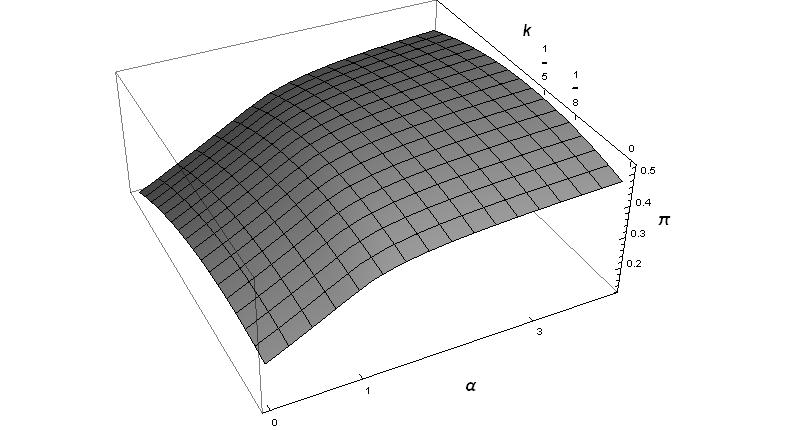
\includegraphics[width=1.0\textwidth]{./figures/Endogenousksimulation0.jpg}
\caption{Simulation of profits with a high cost of piracy }
\flabel{Classic case: Buyers and non-users, }
\label{endk1}
\end{figure}

Similarly we simulate the case where $0<r<\tilde{r}$. Since we now have an additional dimension to represent, we use a 3D contour graph, see figure \ref{endk2}. In this case the $k$ is the optimal k pursued. Notice that once again the equilibrium $k$ is around $\frac{1}{8}$ for low values of product degradation $r$. However, in this scenario, the previous result is reversed, that is, higher piracy pursuit decreases the optimal product improvement. The intuition behind this counterintuitive result is that $r$ and $k$ are substitutes, the firm can use the higher $r$ as an alternative to spending on $k$. In other words, the local effect of an increase in $r$ within $0<r<\tilde{r}$ is to decrease product improvement but once $r=\tilde{r}$, then there is a discontinous jump which depends on the network value which causes an increase in product improvement. 


\begin{figure}[t!] 
\centering
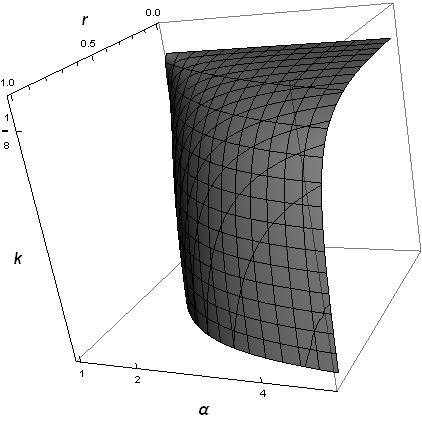
\includegraphics[width=0.5\textwidth]{./figures/Endogenousksimulation.jpg}
\caption{Intermediate cost of piracy case: Contour of the profit function maximized with repspect to the product improvement}
\flabel{Buyers, pirates and non-users}
\label{endk2}
\end{figure}


% In the classic case, where there are no pirates because the cost of piracy is high, the model becomes more complex and has no simple closed form solution for product improvement. If we fix the network value to be equal to base value of the product $\alpha=1+k$, we have that $\tilde{k} = \frac{1}{3 \sqrt{3}} \approx \frac{1}{5}$, numerically this is the highest product improvement that can be pursued, therefore product improvement is maximized when the network value is equal to the base value \footnote{Note that because the cost of product improvement is quadratic, the network value will increase faster than the product improvement, therefore at some point, the equality $\alpha = 1+k$ will hold. If we take the limit of the demand function, $1-\tilde{x}$ with $\alpha$ approaching this parameterization we have that the demand is $\frac{\sqrt{(1+k)(1+k-p)}}{1+k}$. Using this in the profit function, we attain that $p=\frac{2}{27} (9 + \sqrt{3})$ and $k=\frac{1}{3 \sqrt{3}} $ and consequently, profit is, $\pi = \frac{1}{27} \left(1+6 \sqrt{3}\right)$.}.

% In fact even if there is no network value the product improvement pursued is equal the value pursued in the cost-less case,  $\alpha=0 \Rightarrow \tilde{k} = \frac{1}{8}$. Numerically we can also see that as $\alpha$ approaches a large number, $k$ approaches $\frac{1}{9}$
% \footnote{even at $\alpha=100 000 000, k=.1111111$  }. Implying that product improvement peaks when network value is equal to base value. 


% \begin{proposition}
% \label{substitutabilityproposition}
% The network value is substituable with product improvement. 
% \end{proposition}

% \begin{proof}
% See appendix: \ref{substitutabilityproof}
% \end{proof}


% The extra first and second order conditions are given by:

% \begin{equation*}
% \frac{\partial \pi}{\partial k} = \frac{ p(p-r)}{((\alpha-1)
% \sqrt{ 1-r }
% +k)^2} -2k
% \end{equation*}

% \begin{equation*}
% \frac{\partial^2 \pi}{\partial k^2} = -\frac{2 p(p-r)}{((\alpha-1)
% \sqrt{ 1-r }
% +k)^3} -2
% \end{equation*}


% \begin{proposition}
% \label{alphak}
% If $\alpha>1$ then an increase in $\alpha$ can only decrease the pursued product improvement. 
% \end{proposition}

% \begin{proof}
% First we derive with respect to the exogenous variables. Due to the envelope theorem we need only look at the direct effects of the derivative and can ignore indirect effects due to the price. 
% \begin{equation*}
% \frac{\partial \pi }{\partial \alpha} =\frac{\sqrt{1-r}p^* (p^*-r)}{\left((a-1) \sqrt{1-r}+k\right)^2}
% \end{equation*}

% We then proceed to derive with respect to $k$:
% \begin{equation*}
% \frac{\partial^2 \pi }{\partial \alpha k} =
% -\frac{2 \sqrt{1-r} (p^*-r)}{\left((\alpha-1) \sqrt{1-r}+k\right)^3}
% \end{equation*}
% Since this derivative is negative if $\alpha>1$ and $p^*>r$ it implies substitutability between $\alpha$ and k.  
% \end{proof}

% The more intuitive interpretation of proposition \ref{alphak} is simply that the firm will invest to improve the product when the good has a low network value, but as the network value of the good increases, it no longer has need to undertake this investment and since investment is costly, it will just decrease the degree at which it is pursued.

% In the intermediate cost of piracy case, there is once again no closed form solution. Some point estimates, a first and second order approximations are done in the appendix notes(\ref{notes}). However we can deduce how the firm would optimize product improvement with respect to $\alpha$. 

% \begin{corollary}
% Proposition \ref{alphak} implies that the upper bound value of product improvement is $k= \frac{1}{8}$
% \end{corollary}


% To see this corollary we need only note if $\alpha$ was smaller than 1, then the derivative would be positive and therefore the two would be complementary. So the product improvement peaks a $\alpha=1$ and then starts to decrease. In other words, the product improvement pursued when there are no pirates is an upper bound on the intermediate piracy. The firm has a higher incentive to increase the value of its product if pirating is free. 

% \begin{proposition}
% If the network value is large, then further increases in the network value increases the number of buyers. 
% \end{proposition}

% \begin{proof}
% \begin{align*}
% 1 - \hat{x}= 1 - \frac{p-r}{(\alpha - 1) \sqrt{1-r} +k} \\
% = 1 - \frac{k+ (\alpha-1)\sqrt{ 1 -r }-r}{2(\alpha - 1) \sqrt{1-r} +2k} \\
% \frac{\partial (1 - \hat{x})}{\partial \alpha}=  -\frac{ \frac{\partial k}{\partial \alpha}+ \sqrt{ 1 -r }}{2(\alpha - 1) \sqrt{1-r} +2k}+\frac{(k+ (\alpha-1)\sqrt{ 1 -r }-r) (2 \sqrt{1-r}+\frac{\partial k}{\partial \alpha})}{(2(\alpha - 1) \sqrt{1-r} +2k)^2} \\
% =-\frac{\frac{\partial k}{\partial \alpha} \left(\alpha \sqrt{1-r}+k+r-\sqrt{1-r}\right)+2 r\sqrt{1-r} }{4 \left((\alpha-1) \sqrt{1-r}+k\right)^2}
% \end{align*}

% First note that from proposition \ref{alphak} we know that the derivative of k is negative, therefore the whole term is negative if:

% \begin{align*}
% \alpha \sqrt{1-r}+k+r-\sqrt{1-r}<0 \\
% \alpha <1-\frac{k+r}{\sqrt{1-r}}<1 
% \end{align*}

% The above condition never occurs. Because $\alpha>1$ by assumption. 

% We need only check the condition for which the left hand term of the numerator is larger than the right hand term. 
% \begin{align*}
% \alpha>\frac{2 r}{\frac{\partial k}{\partial \alpha}}-\frac{k}{\sqrt{1-r}}-\frac{r}{\sqrt{1-r}}+1 \\
% \end{align*}

% Note that since we know that when $\alpha$ is large, the effect on k approaches 0, this implies that the RHS approaches negative infinity, therefore $\alpha$ increases gradually the proportion of buyers
% \end{proof}

\section{Discussion and Conclusion}
The interpretation so far has been about network goods however a reputation interpretation could work equally well. If we interpret both $\alpha$ and $\beta$ as reputational effects. Both $\alpha$ and $\beta$ can be seen as signalling devices that can only be recognized by the portion of agents who are using. This interpretation may be less intuitive, however it more naturally explains why there may be a differential between the two network values.

The model has been assuming a kind of worse case scenario as to the effect of pirates. Though pirates can be used by the firm to increase its prices, there is no direct revenue mechanism for them. This could easily be imagined in a few cases, for instance, in the digital world a higher use base would allow for indirect profit opportunities. Take a social network as an example, a larger user base allows the network owner to sell advertising slots at a higher price, and the wider the reach the more profitable the enterprise. This kind of mechanism would only strengthen the profits of the firm in the pure piracy case whilist leaving the classic case unaffected. 

Welfare in the model is always decreasing with respect to the cost of piracy. This is simply because the firm mostly does not produce the product since the welfare from an increase in user base is always positive. In the baseline model the product already exists, it only by endogenizing the product improvement that the firm can add value. This does not entail that product degradation should always be zero because profits must be higher than the fixed cost of creating the product. Instead, it should only be noted that the framework presented here actually implies the existence of pareto improving policies. That is, when the network value is high the firm prefers there to be a higher amount of piracy over no piracy at all. 

% In the standard literature, the only source of revenue for a firm is to sell the product. However there are situations, especially in the digital world where having a larger user base also allows for additional indirect profit opportunities. For instance in a social network, a larger user base allows the network owner to sell advertising slots at a higher price, and the wider the reach the more profitable the enterprise. This extra source of revenue is parametrized with the letter $\lambda$. It should be noted that increasing pirates or buyers increase revenue from this source. 

Our model shows that even if the firm has total control of the level of piracy pursuit, it would not necessarily fully utilize this capability. Under the conditions discussed above, the firm often has incentive to not use deterrence to push consumers out of its pool of customers because reducing the number of consumers also decreases the value of the good for those who would buy. The intuition behind this carrot and stick approach is that the price has a single effect whilst piracy pursuit has a double effect. The price effect is less variable because it gives the firm the ability to be more precise in its targeting mechanism. Wile changing the price only works on the consumers who are marginally on the edge of the choice of buying or pirating, changing the degradation level affects all segments at once, resulting in more global network effects. 

Increasing the product degradation affects both the proportion of users buying while also decreasing the user base. The strength of these two effects depends on their valuation of the network value. The decrease in the user base corresponds to the product becoming less popular and the change in buying behavior represents either a consumer who no longer wishes to undertake the risk of pirating or a consumer who no longer wishes to buy the product because it has less value to her.

Though the more traditional way of seeing pirates is as a competitive force, in the model presented here pirates take the role of the path of least resistance. Indeed controlling the pirates to ensure that they are at the right level is a fine art and the if the instrument is too blunt, it may cause more harm than good. The conditions for piracy to be optimal are relatively mild, the bought network value need only reach a certain threshold for it to be worthwhile. Indeed though the model assumed that pursuing pirates is costless, in the real world, there are significant costs both from the point of view of the planner and the firm. The endogenization of these costs would only decrease the threshold $\alpha$ for which the firm would prefer piracy to exist.

One simple policy implication of the model is that pursuing pirates uniformly for all their activities may have welfare reducing effects. An optimal solution would be one where the pursuit of piracy is  heterogeneous to each firm. Much like how firms only sue specific infringers and let others go, the same can be encouraged on the consumer side. From the legal point of view the implication is that piracy could be viewed as a civil or corporate issue and not a criminal one. For broadening the scope of tort law, see \citep{DF96}. 

Still, this approach is limited in that, whilst it is possible for a firm to identify other infringers and selectively sue them, it is likely that the number of pirates is too high to accurately identify. However, if we are to include the cost of identification, this same cost has to be applied on any mechanism that enforces piracy laws. A policy that focuses on enforcement against consumers is likely to have a much higher social cost than one which is enforced on firms in accordance with the actual number of consumers. 

Put in another way, the problem with copyright enforcement is that it is unconditional. That is, unlike patents, where the patent right holder chooses to initiate an action against a patent infringer, presumably following a calculation which leads the patent right holder to the conclusion that such an action is worthwhile. The illegal act of piracy is unconditionally a criminal offense. In other words, regardless of whether the effects of the act aid or harm a copyright owner there is a consistent social cost imposed. 

In practice, firms cannot control the probability of success when initiating an action. In industries where the pirates are many and are highly decentralized, it is quite plausible that neither the government nor the firms can greatly increase their level of piracy pursuit without greatly invading personal data and privacy laws. Realistically, cases involving music or movies are more adapted and fit better into the above developed model. 

It is also important to note that there are firm adaptation which can be used as alternatives to the law. These strategies may be less costly because they can focus on prevention rather than pursuit. In the digital space, these strategies are usually labeled, Digital Rights Management (DRM) strategies. Examples of DRM are idea's such as requiring users to use specific platforms to access the content, monitoring consumption, selling restricted usage copies etc. Such strategies may be complementary or substitutable with piracy enforcement. DRM strategies allow firms to select their own level of piracy pursuit. Piracy often has its own platforms which continously improve their own services. Indeed much of the historic incentive to pirate was due to the superior platform services of piracy software. The new wave of streaming services such as Netflix or Amazon prime represent competition to these piracy services.


A hidden assumption in the model presented above is that all users value socializing with all other users. In the real world, if there are segregation effects, this assumption may not be fully applicable. On the other hand, if we assume that segregation brings together more diverse valuations, such as perhaps a family unit, then this solidifies the conclusions of this model.

Generally, the assumption that utilities are independent is often too readily used. What is termed a "network good" in the industrial organization literature can be interpreted too narrowly. It is not simply digital social networks that have this property. In fact, it is possible to envision most goods as having both an intrinsic value and an extrinsic component. The relative ratio of intrinsic to extrinsic value will likely vary substantially between cultures, space and time. Additionally, the domain in which this is true is likely to extend much farther than what common intuition would entail. For instance, even perishable goods, such as food, are not necessarily exempt from this feedback process, for instance the consumption of cheese or wine is not something that is independent of the surrounding culture. Accordingly, much of what can be deemed "group identity" can be represented within a network good framework. A culture of baguette or chocolate eaters does not represent the same profit opportunities as groups without such culture.

One of the most common arguments against piracy is that it decreases the number of individuals who actually pay the real cost of the product.  However, the implicit assumption in such a line of reasoning is that the number of purchasers and the value of the purchasing, are independent. Based on the model presented here, such a conclusion is drawn too hastily, the effect of increasing the piracy cost may not have the desired effect. As pointed out in \cite{CRP91} this setup raises strange ethical questions. When we have possible parameter values that imply that higher pursuit of pirates may be worse for consumers and producers at public cost. With these factors in mind, it is unclear whether enforcing intellectual property rights passes even the most basic cost benefit analysis.

\newpage
\section{Appendix}
\subsection{Buyers and pirates}
\begin{equation*}
\hat{x} = \frac{p}{\alpha-\beta + k}
\end{equation*}

The upper condition is $\alpha-\beta+k \geq p$. Therefore the price is:

\begin{equation*}
p = \frac{1}{2}\left(
\alpha-\beta+k
\right)
\end{equation*}

Note that these values imply that $\hat{x} = \frac{1}{2}$ regardless of the values of $\beta$ or $\alpha$. Profit is then:
\begin{align*}
\pi &= p(1-\hat{x}) \\
&=  \frac{1}{4}\left(
\alpha-\beta+k
\right)  \\
\end{align*}

Social Surplus and welfare are:
\begin{align*}
\hat{S} &= \int_0^{\hat{x}}x(1+\beta)dx+
\int_{\hat{x}}^{1}\left( x(1+\alpha+k)-p \right)dx \\
&= \frac{1}{8} (\alpha+2 \beta+k+3) \\
\hat{W} &= \frac{3}{8} \left( 1 + \alpha +k
\right)
\end{align*}



\subsection{Proof of proposition \ref{buyersusersprice}} \label{buyersuserspriceproof}

\begin{align*}
\textbf{The demand function in the case of buyers only is given by:} \\
1-\frac{\alpha+k+1-\sqrt{(-\alpha-k-1)^2-4 \alpha p}}{2 \alpha} \\
\frac{\alpha-k-1+\sqrt{(-\alpha-k-1)^2-4 \alpha p}}{2 \alpha}
\\
\textbf{The profit function is then:} 
\\
p*\frac{\alpha-k-1+\sqrt{(-\alpha-k-1)^2-4 \alpha p}}{2 \alpha}
\\
\text{Derivative with respect to p}: \\
\frac{\sqrt{(\alpha+k+1)^2-4 \alpha p}+\alpha-k-1}{2 \alpha}-\frac{p}{\sqrt{(\alpha+k+1)^2-4 \alpha p}} =0
\\
\frac{\sqrt{(\alpha+k+1)^2-4 \alpha p}+\alpha-k-1}{2 \alpha} =\frac{p}{\sqrt{(\alpha+k+1)^2-4 \alpha p}} \\
%%%%%%%%%%%%%%%%%%%%%%%%%%%%%%%%%%%
( \alpha+k+1)^2-4 \alpha p+(\alpha-k-1)\sqrt{(\alpha+k+1)^2-4 \alpha p} = 2 p \alpha \\
( \alpha+k+1)^2+(\alpha-k-1)\sqrt{(\alpha+k+1)^2-4 \alpha p} = 6 p \alpha \\
%%%%%%%%%%%%%%%%%%%%%%%%%%%%%%%%%%%%%
(\alpha-k-1)\sqrt{(\alpha+k+1)^2-4 \alpha p} = 6 p \alpha - ( \alpha+k+1)^2 \\
%%%%%%%%%%%%%%%%%%%%%%%%%%%%%%%%%%%
(\alpha-k-1)^2((\alpha+k+1)^2-4 \alpha p) = (6 p \alpha - ( \alpha+k+1)^2 )^2
%%%%%%%%%%%%%%%%%%%%%%%%%%%%%
% \\
% (\alpha-k-1)^2(\alpha+k+1)^2-(\alpha-k-1)^2 4 \alpha p = 36 p^2 \alpha^2 + ( \alpha+k+1)^4 - 12 p \alpha ( \alpha+k+1)^2 
% \\
% 0 = 36 p^2 \alpha^2  +4 p \alpha((\alpha-k-1)^2-3( \alpha+k+1)^2) + ( \alpha+k+1)^2(( \alpha+k+1)^2-(\alpha-k-1)^2)
% \\
% 0 = 36 p^2 \alpha^2  +4 p \alpha((\alpha-k-1)^2-3( \alpha+k+1)^2) + ( \alpha+k+1)^2(4 \alpha(1+k))
\\
0 = 9 p^2 \alpha  -2 p (\alpha^2 + 4\alpha(1+k)+(1+k)^2) + ( \alpha+k+1)^2 (1+k)
\\
\textbf{This is gives two solutions for p:} \\
\tilde{p} = \frac{(\alpha+k+1)^2+2\alpha(k+1) \pm \sqrt{(1-\alpha+k)^2(\alpha^2+\alpha (k+1)+(k+1)^2)}}{9 \alpha} \\
 = \frac{(\alpha+k+1)^2}{9 \alpha}+\frac{2(1+k)}{9}+\frac{ \pm \sqrt{(1-\alpha+k)^2(\alpha^2+\alpha (k+1)+(k+1)^2)}}{9 \alpha} \\
\end{align*}

If $\alpha$ is large relative to $1+k$, the expression simplifies, we will represent the use of this assumption by $\approx$. 

\begin{align*}
p \approx \frac{\alpha}{9}+\frac{2(1+k)}{9}+\frac{ \pm \sqrt{(\alpha^2+\alpha (k+1))}}{9 } \\
=\frac{\alpha}{9}+\frac{2(1+k)}{9}+\frac{ \pm \sqrt{(\alpha^2+\alpha^2 \frac{(k+1)}{\alpha})}}{9 } \\
=\frac{\alpha}{9}+\frac{2(1+k)}{9}+\frac{ \pm \alpha \sqrt{ \frac{k+1+\alpha}{\alpha}}}{9} \\
=\frac{2\alpha}{9}+\frac{2(1+k)}{9}
\end{align*}


\subsubsection{corollary:}
\label{squareroot}

\begin{align*}
&\sqrt{(\alpha+k+1)^2-4 \alpha p} \\
&\text{Substitute in the approximated price:} \\
&\approx\frac{1}{3} \sqrt{a^2+10 a (k+1)+9 (k+1)^2} \\
&\approx \frac{1}{3} \sqrt{a^2+10  \frac{a^2}{a} (k+1)} \\
&\approx \frac{a}{3} \sqrt{1+ \frac{10}{a} (k+1)} \\
&\approx  \frac{a}{3}
\end{align*}

We can use this expression to represent the proportion of agents who will consume in equilibrium:

\begin{align}
1-\tilde{x} &= 1-\frac{\alpha+k+1-\frac{a}{3}}{2 \alpha} \\
&=\frac{4\alpha-3(1+k)}{6\alpha}
\approx \frac{2}{3}
\end{align}


\subsection{Proof of proposition \ref{piracyvsnotproposition}} \label{piracyvsnot}

We now look at the what the derivative of the profit function turns out to be. First note that in proposition \ref{envelopetheorem} we deduce that the envelope theorem applies. We also use corollary \ref{squareroot} to simplify the square root and proposition to have the simplified price which assume that $\alpha$ is large. 

\begin{align*}
\frac{\partial f}{\partial \alpha} = \frac{\frac{2 (\alpha+k+1)-4 p}{2 \sqrt{(\alpha+k+1)^2-4 \alpha p}}+1}{2
   \alpha}-\frac{\sqrt{(\alpha+k+1)^2-4 \alpha p}+\alpha-k-1}{2 \alpha^2} \\
=\frac{1}{2 \alpha}
\left( 
\frac{2 (\alpha+k+1)-4 p}{2 \sqrt{(\alpha+k+1)^2-4 \alpha p}}+1-\frac{\sqrt{(\alpha+k+1)^2-4 \alpha p}+\alpha-k-1}{ \alpha}
\right) \\
=\frac{1}{2 \alpha}
\left( 
\frac{ (\alpha+k+1)-2 p}{ \sqrt{(\alpha+k+1)^2-4 \alpha p}}-\frac{\sqrt{(\alpha+k+1)^2-4 \alpha p}-k-1}{ \alpha}
\right) \\
=\frac{1}{2 \alpha}
\left( 
\frac{ \alpha (\alpha+k+1)-2 \alpha p}{ \alpha\sqrt{(\alpha+k+1)^2-4 \alpha p}}-\frac{\sqrt{(\alpha+k+1)^2-4 \alpha p}(\sqrt{(\alpha+k+1)^2-4 \alpha p}-k-1)}{ \alpha\sqrt{(\alpha+k+1)^2-4 \alpha p}}
\right) \\
% =\frac{1}{2 \alpha}
% \left( 
% \frac{ \alpha (\alpha+k+1)-2 \alpha p}{ \alpha\sqrt{(\alpha+k+1)^2-4 \alpha p}}-\frac{\sqrt{(\alpha+k+1)^2-4 \alpha p}(\sqrt{(\alpha+k+1)^2-4 \alpha p}-k-1)}{ \alpha\sqrt{(\alpha+k+1)^2-4 \alpha p}}
% \right) \\
% =\frac{1}{2 \alpha^2 \sqrt{(\alpha+k+1)^2-4 \alpha p}}
% \left( 
% \alpha (\alpha+k+1)-2 \alpha p-\sqrt{(\alpha+k+1)^2-4 \alpha p}(\sqrt{(\alpha+k+1)^2-4 \alpha p}+k+1)
% \right) \\
% =\frac{1}{2 \alpha^2 \sqrt{(\alpha+k+1)^2-4 \alpha p}}
% \left( 
% \alpha (\alpha+k+1)-2 \alpha p-(\alpha+k+1)^2+4 \alpha p+(k+1)\sqrt{(\alpha+k+1)^2-4 \alpha p})
% \right) \\
% =\frac{1}{2 \alpha^2 \sqrt{(\alpha+k+1)^2-4 \alpha p}}
% \left( 
% \alpha (\alpha+k+1)-(\alpha+k+1)^2+2 \alpha p+(k+1)\sqrt{(\alpha+k+1)^2-4 \alpha p})
% \right) \\
% =\frac{1}{2 \alpha^2 \sqrt{(\alpha+k+1)^2-4 \alpha p}}
% \left( 
% -(1+k)(\alpha+k+1)^2+2 \alpha p+(k+1)\sqrt{(\alpha+k+1)^2-4 \alpha p})
% \right) \\
=\frac{1}{2 \alpha^2 \sqrt{(\alpha+k+1)^2-4 \alpha p}}
\left( 
2 \alpha p+(k+1)(\sqrt{(\alpha+k+1)^2-4 \alpha p})-(\alpha+k+1)^2)
\right) \\
\textbf{We now assume that $\alpha$ is large relative to k+1 and substitute in the price and square root}
\\
=\frac{3}{2 \alpha^3 }
\left( 
2 \alpha p+(k+1)(\frac{a}{3}-(\alpha+k+1)^2)
\right) \\
=\frac{3}{2 \alpha^3 }
\left( 
2 \alpha (\frac{2\alpha}{9}+\frac{2(1+k)}{9})+(k+1)(\frac{a}{3}-(\alpha+k+1)^2)
\right)
\\
=\frac{3}{2 \alpha^3 }
\left( 
\frac{4\alpha^2}{9}+\frac{4\alpha(1+k)}{9}+(k+1)(\frac{a}{3}-(\alpha+k+1)^2)
\right)\\
=\frac{3}{18 \alpha^3 }
\left( 
4\alpha^2+4\alpha(1+k)+(k+1)(\frac{a}{3}-(\alpha+k+1)^2)
\right)\\
\textbf{Multiply by the price}
\\
p(a)\frac{\partial f}{\partial \alpha} = (\frac{2\alpha}{9}+\frac{2(1+k)}{9})\frac{3}{18 \alpha^3 }
\left( 
4\alpha^2+4\alpha(1+k)+(k+1)(\frac{a}{3}-(\alpha+k+1)^2)
\right)\\
= \frac{\alpha +1+k}{27 \alpha^3 }
\left( 
4\alpha^2+4\alpha(1+k)+(k+1)(\frac{a}{3}-(\alpha+k+1)^2)
\right)
\\
= \frac{\alpha +1+k}{27 \alpha^3 }
\left( 
4\alpha^2+(k+1)(\frac{13a}{3}-(\alpha+k+1)^2)
\right)\\
\end{align*}

\begin{align*}
\text{If alpha is large relative to k+1}\\
= \frac{\alpha}{27 \alpha^3 }
\left( 
4\alpha^2+(k+1)(\frac{13a}{3}-\alpha^2)
\right)
\\
= \frac{1}{27 \alpha^2 }
\left( 
4\alpha^2+(k+1)(\frac{13a}{3}-\alpha^2)
\right) \\
= \frac{1}{27 \alpha^2 }
\left( 
4\alpha^2+(k+1)\frac{\alpha}{3}(13-3 \alpha)
\right)
\\
= \frac{1}{71 \alpha }
\left( 
12\alpha+(k+1)(13-3 \alpha)
\right) \\
\text{If the second term is negative, which occurs after $\alpha$ exceeds 5 we can say}
\\
= \frac{1}{71 \alpha }
\left( 
12\alpha+(k+1)(13-3 \alpha)
\right) < \frac{12}{71 }
\end{align*}
Recall that the slope of the profit function with pirates is $\frac{1}{4}$, therefore profit under piracy increases more than profit without piracy if $\alpha$ is relatively large


% \subsection{Proof of proposition \ref{substitutabilityproposition} }

% \label{substitutabilityproof}

% \begin{proof}
% First note that the cross partial derivative is given by:
% \begin{equation*}
% \frac{\partial^2 \pi}{\partial \alpha k} =
% \frac{p \left(-\frac{\alpha+k+1}{\sqrt{(\alpha+k+1)^2-4 \alpha p}}-\frac{2 \alpha p (\alpha-k-1)}{\left((\alpha+k+1)^2-4 \alpha p\right)^{3/2}}+1\right)}{2 \alpha^2} 
% \end{equation*}

% To check the sign we need only see that the two first terms inside the parenthesis are decreasing in $\alpha$. 
% \begin{align*}
% &= \left(-\frac{\alpha+k+1}{\sqrt{(\alpha+k+1)^2-4 \alpha p}}-\frac{2 \alpha p (\alpha-k-1)}{\left((\alpha+k+1)^2-4 \alpha p\right)^{3/2}}+1\right)&& \\
% %%%%%%%%%%%%%%%%%%%%%%%%%%%%%%%%%
% &= 1- \frac{2 \alpha p (\alpha-k-1)+((\alpha+k+1)^2-4 \alpha p)(1+k+\alpha)}{\left((\alpha+k+1)^2-4 \alpha p\right)^{3/2}}& \\
% %%%%%%%%%%%%%%%%%%%%%%%%%%%%%%%%%
% &= \frac{\left((\alpha+k+1)^2-4 \alpha p\right)^{3/2}-2 \alpha p (\alpha-k-1)-((\alpha+k+1)^2-4 \alpha p)(1+k+\alpha)}{\left((\alpha+k+1)^2-4 \alpha p\right)^{3/2}}& \\
% %%%%%%%%%%%%%%%%%%%%%%%%%%%%%%%%%
% &=\frac{\left((\alpha+k+1)^2-4 \alpha p\right)^{3/2}+2 \alpha p (\alpha-3(k+1))-((\alpha+k+1)^3}{\left((\alpha+k+1)^2-4 \alpha p\right)^{3/2}} &
% \end{align*}*

% Note that if $\alpha=0$ then the cross partial is 0. Then note that in the last expression, the last term is always larger than the first term when $k>0,\alpha>0, p>0$. Then note that the second term is negative whenever $\alpha<3$ and if $\alpha>3$ then the cube route effect of the last term dominates.  
% \end{proof}

\subsection{Proof of proposition \ref{tdemand}}

\label{tdemandp}

We first begin with the condition which renders an agents indifferent between pirating and not using to solve for the valuation $x$ of the indifferent pirate. 


\begin{align*}
x(1+\beta(1-F(x)))-r=0 \\
x(1+\beta(1-x))=0 \\
x+x\beta-\beta x^2-r=0 \\
x^2-x\frac{(1+\beta)}{\beta} +\frac{r}{\beta} = 0 \\
\check{x} = \frac{(1+\beta)}{2 \beta}
\pm
\frac{ \sqrt{ \left(\frac{(1+\beta)}{\beta}\right)^2 -4\frac{r}{\beta} } }{2} \\
\check{x} = \frac{(1+\beta)}{2 \beta}
\pm
\frac{ \sqrt{ \left(1+\beta\right)^2 -4r\beta } }{2 \beta} \\
\end{align*}



\begin{equation*}
\check{x} = 1
\pm \sqrt{ 1 -r }
\end{equation*}

If $\check{x}>1$ is verified this implies that no users will be pirating since all users prefer not to pirate. Therefore only the negative solution can be used.  With the indifferent user, we need only take the difference $1-\check{x}$ to know the proportion of agents who are users. This proportion is simply:

\begin{align*}
1-\check{x}=\sqrt{ 1 -r }
\end{align*}

We note that the proportion of agents who are users is entirely exogenous to the firm. What is endogenous to the firm is the proportion of agents who are buyers. The proportion of agents who are buyers, ceteris parabus, depends on the proportion who are pirates. The consumer who is indifferent between purchasing and pirating can similarly be found by equating the two options. Which gives the following value:

\begin{align*}
x(1+\beta(1-F(x)))-r=x(1+\alpha(1-F(x)))-p \\
\Rightarrow \hat{x}=\frac{p-r}{(\alpha-1)\sqrt{ 1 -r }+k} \\
\end{align*}

Where the last step occurs because $1-F(x)=1-\check{x}$. Recall that $\hat{x} \geq \check{x}$ from the preliminary section. The demand function for buying can then simply be written as:

\begin{align*}
D(\hat{x})=1-\hat{x}=1-\frac{ (p-r)}{k + (\alpha-1) \sqrt{ 1 -r }} \\
%%%%%%%%%%%%%%%%%%%%%%%%%%%%%%%%
\frac{\partial D(\hat{x})}{\partial p} =
-\frac{ 1}{k + (\alpha-1) \sqrt{ 1 -r }} \\
%%%%%%%%%%%%%%%%%%%%%%%%%%%%%%%%%
\frac{\partial D(\hat{x})}{\partial k} =
\frac{ (p-r) }{(k+
 (\alpha-1)\sqrt{ 1 - r }
)^2} 
%%%%%%%%%%%%%%%%%%%%%%%%%%%%%%%%%
%%%%%%%%%%%%%%%%%%%%%
\end{align*}

% This condition must satisfy that the higher indifferent agent must have a lower valuation, $x$ than the highest valuation user, $\hat{x} \leq 1$. This constraint can be used to give us an upper bound on the price the firm can charge. We call this condition 1, $C_1$

% \begin{align*}
% \hat{x} \leq 1 \\
% \frac{p-r}{(\alpha-1)\sqrt{ 1 -r }+k} \leq 1
% \\
% p \leq (\alpha-1)\sqrt{ 1 -r }+k+r \\
% \text{or we can get an upper bound on k} \\
% p -(\alpha-1)\sqrt{ 1 -r } -r\leq k \\
% \text{similarly we can use the lower bound:} \\
% \hat{x} \geq 0 \\
% \frac{p-r}{(\alpha-1)\sqrt{ 1 -r }+k}  \geq 0 \\
% p \geq r
% \end{align*}

% We similarly recall that the indifferent consumer between buying and pirating must be higher than the indifferent consumer between pirating and not buying, $\hat{x}>\check{x}$. We can use this condition to get a further condition.  We call this the second condition $C_2$
% \begin{align*}
% C_2 = \frac{p-r}{(\alpha-1)\sqrt{ 1 -r }+k} -\sqrt{ 1 -r } \geq 0
% \\
% \frac{p-r}{(\alpha-1)\sqrt{ 1 -r }+k} 
% \geq
% \sqrt{ 1 -r } \\
% p-r
% \geq \sqrt{ 1 -r }((\alpha-1)\sqrt{ 1 -r }+k) \\
% p-r
% \geq (\alpha-1)( 1 -r )+k\sqrt{ 1 -r } \\
% p
% \geq \alpha -1+r(2-\alpha)+k\sqrt{ 1 -r }
% \end{align*}

% We can compare this constraint to the previous one to see that this one is stricter:

% \begin{align*}
% -1+r(2-\alpha)+k\sqrt{ 1 -r } \geq r \\
% \Rightarrow
% k\sqrt{ 1 -r } + (1 -r)(\alpha-1) \geq 0
% \end{align*}








\section{Endogenous k}


\subsection{case where $r=0$}

\begin{proposition}
If $r=0$, the firm will choose $(p,k)=(\frac{1}{16c}+\frac{\alpha-\beta}{2},\frac{1}{8c})$ $\check{x}=0$ and $\hat{x}=1/2$ and $\pi= \frac{1}{4}(\alpha-\beta)+\frac{1}{64c}$.
\end{proposition}

\begin{proof}


As in the exogenous case we solve for the indifference condition:

\begin{align*}
\hat{x}(1+\alpha+k)=\hat{x}(1+\beta) \\
\Rightarrow \hat{x} = \frac{p}{\alpha - \beta +k}
\end{align*}


Now, the profit function is

\begin{equation*}
\tilde{\pi} = p\left(1-\frac{p}{\alpha - \beta +k}\right)-c k^2
\end{equation*}

The two first order conditions, relatives to $p$ and $k$, for the profit maximization are:

\begin{align*}
\frac{\partial \tilde{\pi}}{\partial p}= 1-\frac{2p}{\alpha - \beta +k}\\
\frac{\partial \tilde{\pi}}{\partial k}=  \frac{p^2}{(\alpha-\beta+k)^2}-2ck 
\end{align*} 

\begin{equation*}
p = \frac{\alpha-\beta-k}{2}
\end{equation*}

and 

\begin{equation*}
2ck = \frac{p^2}{(\alpha-\beta+k)^2}
\end{equation*}

This gives $k^*=\frac{1}{8c}$,  and $p^*=\frac{\alpha-\beta}{2}+\frac{1}{16c}$ and $\pi=\frac{1}{4}(\alpha-\beta)+\frac{1}{64c} $ if we put these values in the profit equation. 

\end{proof}

\begin{observation}
The product improvement chosen by the firm does not depend on network values, $\beta$ and $\alpha$
\end{observation}


\subsection{Intermediate r}
$0<r<\tilde{r}$

We need to also verify that the profit function satisfies the first and second order conditions with respect to the price level.

\begin{align*}
\pi = p\left(1-\hat{x}\right) - k^2 \\
%%%%%%%%%%%%%%%%%%%%%
=p\left(1-\frac{ (p-r)}{(\alpha-1)
\sqrt{ 1-r }
+k} \right) -k^2
\\
%%%%%%%%%%%%%%%%%%%%%
\frac{\partial \pi }{\partial p} = 1-\frac{ (2p-r)}{
k+ (\alpha-1)\sqrt{ 1 -r }} \\
%%%%%%%%%%%%%%%%%%%%%
\frac{\partial^2 \pi }{\partial p^2}
= -\frac{ 2}{
k+ (\alpha-1)\sqrt{ 1 -r }} \\
%%%%%%%%%%%%%%%%%%%%%
%%%%%%%%%%%%%%%%%%%%%
%%%%%%%%%%%%%%%%%%%%%
\frac{\partial \pi}{\partial k} = \frac{ p(p-r)}{((\alpha-1)
\sqrt{ 1-r }
+k)^2} -2k
\\
%%%%%%%%%%%%%%%%%%%%%
\frac{\partial^2 \pi}{\partial k^2} = -\frac{2 p(p-r)}{((\alpha-1)
\sqrt{ 1-r }
+k)^3} -2 
\end{align*}

\subsection{Some values for k}

We now set $ (\alpha-1)\sqrt{ 1 -r }=w$ and proceed to solve for $k$ using the second FOC.  

\begin{align*}
\frac{\partial \pi}{\partial k} = \frac{ p(p-r)}{(w
+k)^2} -2k \\
2k= \frac{ p(p-r)}{(w
+k)^2} \\
2k(w+k)^2=p(p-r) \\
\text{We now substitute the price into the this: } \\
2k(w+k)^2=\frac{k+ w+r}{2} \left(\frac{k+ w+r}{2}-r \right) \\
2k(w+k)^2=\frac{k+ w+r}{2} \left(\frac{k+ w-r}{2} \right) \\
8k(w+k)^2= \left( k+ w+r \right) \left(k+ w-r\right) \\
\text{If we assume that $w=r$} \\
\Rightarrow 
k = \frac{1}{16} \left(1\pm \sqrt{32 r+1}\right) - r\\
\text{Only the positive solution yields positive values} \\
= \frac{1}{16} \left(1\pm \sqrt{32 r+1}\right) - r \\
\text{This function is maximized at $k=\frac{1}{8}$} \\
\text{We now take a limit case as $\alpha$ increases:} \\
8k(w+k)^2= \left( w+ k \right)^2 \\
k = \frac{1}{8} \\
\text{Similarly if:} \\
\alpha=1=\beta \\
\Rightarrow w = 0 \\
\Rightarrow k = \frac{1}{8} 
\end{align*}

\subsection{Notes} \label{notes}

\subsubsection{Why the envelope theorem applies} \label{envelopetheorem}


For notational simplicity we represent the demand function which is a function of $\alpha, p, k$ as $l(a, k(a),p(a))$.  

\begin{align*}
\pi(a, p(a),k(a))= p(a) l(a, k(a),p(a))-k(a)^2 \\
%%%%%%%%%%%%%%%%%%%%%%%%%%%%%%%%
\frac{ \partial \pi(a, p(a),k(a))}{\partial \alpha}= \frac{\partial p(a) }{\partial a } \left(
l(a, k(a),p(a)) \right)
+ p(a)\left( \frac{\partial l}{\partial a}
+\frac{\partial l}{\partial k(a)}\frac{\partial k(a)}{\partial a}
+\frac{\partial l}{\partial p(a)}\frac{\partial p(a)}{\partial a}
\right)
- 2 k(a) \frac{\partial k(a)}{\partial a}
\\ 
%%%%%%%%%%%%%%%%%%%%%%%%%%%
= \frac{\partial p(a) }{\partial a } \left(
l(a, k(a),p(a)) +p(a) \frac{\partial l}{\partial p(a)} \right)
+ p(a) \frac{\partial l}{\partial a}
+\frac{\partial k(a)}{\partial a}\left( p(a)\frac{\partial l}{\partial k(a)}-2 k(a)
 \right) \\
FOCS: 
\\
\frac{\partial \pi(a, p(a),k(a))}{\partial p(a)}=l(a, k(a),p(a))+p(a) \frac{\partial l}{\partial p(a)}=0 
\\
\frac{\partial \pi(a, p(a),k(a))}{\partial k(a)}=p(a) \frac{\partial l}{\partial k(a)} -2 k(a)=0
\\
\textbf{applying the FOC's we can simplify to}
\\
\frac{ \partial \pi(a, p(a),k(a))}{\partial \alpha}= 
p(a) \frac{\partial l}{\partial a} \\
\end{align*}

Therefore we can deduce the effects of $\alpha$ by simply taking the direct derivative of the profit function. The argument is equivalent for $r$.

\subsubsection{Regularly varying functions}

\begin{definition}
A regularly varyng function $L: (0,+ \infty) \rightarrow (0,+ \infty)$ has the following property:
\begin{equation}
lim_{x \rightarrow \infty} \frac{L(t x)}{L(x)} = g(t)
\end{equation}
\end{definition}

It is known that in regular varying functions, $g(t)$ take the following form\citep{bojanic1963slowly}:
\begin{equation}
g(t)=t^i
\end{equation}

If $g(t)= t$ this implies that the function is eventually linear. 

\begin{align}
L(x)-L(a x) = L(x) - f(a)L(x) = L(x)(1-f(a)) \\
L(y)-L(b y) = L(y) - f(b)L(y) = L(y)(1-f(b)) \\
\text{Linearity  implies:}
x-ax = y-yb \\
\rightarrow y = x \frac{(1-a)}{(1-b)} \\
\rightarrow L\left(x \frac{1-a}{1-b}\right)[1-f(b)] \\
\rightarrow f\left( \frac{1-a}{1-b}\right)L(x)[1-f(b)] \\
\text{L is linear in x if} \\
L(x)f\left(\frac{1-a}{1-b}\right)(1-f(b)) = L(x)(1-f(a)) \\
f\left(\frac{1-a}{1-b} \right) = \frac{1-f(a)}{1-f(b)} \\
\left(\frac{1-a}{1-b} \right)^i = \frac{1-a^i}{1-b^i} 
\end{align}

Which is satisfied because $g(t)=t$ implies $i=1$

\subsubsection{Welfare}

Welfare is just the sum of the social surplus and the profit.

\begin{align*}
W_{bn} = \int^{\tilde{x}}_0 \left(x(1+\alpha(1-\tilde{x})+\tilde{k})-\tilde{p} \right) dx + \tilde{\pi}  \\
W_{bp} = \int^{\hat{x}}_0 x(1+\beta) dx +\int^{1}_{\hat{x}} \left(x(1+\alpha+\hat{k}) - \hat{p} \right) dx + \hat{\pi} \\
W_{bpn} =
\int^{\hat{x}}_{\check{x}} \left(x(1+\beta(1-\check{x}))-r \right)dx +\int^{1}_{\hat{x}} \left(x(1+\alpha(1-\check{x})+\check{k}) - \check{p} \right) dx + \check{\pi}
\end{align*}

\subsubsection{First and second order approximations of endogenous k}

\begin{align*}
\text{If we don't take the limit case then this is:} \\
8k(w+k)^2= \left( w+k \right)^2 -r^2 \\
(w+k)^2(8k-1)=-r^2 \\
\text{If we take a first order approximation:} \\
f(k)= (w+k)^2(8k-1)+r^2 
\\
\approx f(t)+f'(t)(k-t) \\
=(8 t-1) (t+w)^2+r^2 
+(8 (t+w)^2+2 (8 t-1) (t+w))(k-t) \\
\Rightarrow k = \frac{2 t+w^2+2 w-15 t^2-14 t w-r^2}{8 (t+w)^2}
\\
\text{If we approximate around $t=\frac{1}{8}$} \\
k = \frac{(8 w+1)^2-64 r^2}{8 (8 w+1)^2} 
\\
\text{If we approximate around $t=0$} \\
k= \frac{w (w+2)-r^2}{8 w^2}
\\
\text{So k is decreasing with r} \\
\end{align*}

\begin{align*}
\text{A second order approximation of the function:} \\ 
f(k)= (w+k)^2(8k-1)+r^2 \\
\approx f(t)+f'(t)(k-t)+\frac{f''(\alpha)}{2}(k-t)^2 \\
= (8 t-1) (t+w)^2+r^2 
+(8 (t+w)^2+2 (8 t-1) (t+w))(k-t) \\
+\frac{32 (t+w)+2 (8 t-1)}{2}(k-t)^2 \\
= (8 t-1) (t+w)^2+r^2 
+(8 (t+w)^2+2 (8 t-1) (t+w))(k-t) \\
+(16 (t+w)+ (8 t-1))(k-t)^2 
\end{align*}



%\begin{equation*}
%k = \frac{\pm \sqrt{\left(2 t-40 t^2-16 %t w+8 w^2\right)^2-4 (24 t+16 w-1) %\left(r^2+24 t^3+16 t^2 w+14 t^2+14 t %w-2 t-w^2-2 w\right)}+40 t^2+16 t w-2 %t-8 w^2}{2(24 t+16 w-1)} 
%\end{equation*}
We solve for k around 0: 

\begin{align*}
k = \frac{\pm \sqrt{\left(8 w^2\right)^2-4 (16 w-1) \left(r^2-w^2-2 w\right)}-8 w^2}{2(16 w-1)} \\
=\frac{\pm 2 \sqrt{16 w^4- (16 w-1) \left(r^2-w^2-2 w\right)}-8 w^2}{2(16 w-1)} \\
=\frac{\pm \sqrt{16 w^4- (16 w-1) \left(r^2-w^2-2 w\right)}-4 w^2}{16 w-1} \\
\text{only the positive solution gives a positive answer:} \\
= \frac{ \sqrt{16 w^4- (16 w-1) \left(r^2-w^2-2 w\right)}-4 w^2}{16 w-1}
\end{align*}







% \chapter{Cost-side innovation with project variance}
% \section{Introduction}

Models suggest that the possibility for a larger firm to purchase a smaller firm will incentivize smaller firms to innovate. Since this buyout is voluntary, it can only mean that the entrepreneur in question gains. It is difficult to argue against the proposition that increasing the reward of an activity encourages that activity. However this possibility, does not mean that the entrepreneur is more likely to invest in all projects. Quite the contrary, as the possibility increases the incentive to pursue some projects, it simultaneously decreases the incentive to pursue other projects. This paper explores the concept that entrepreneurs are incentivized to pursue projects which are correlated to existing firms activities.
%\textcolor{orange}{Posing the question, what is the relationship buyouts and innovation}


Empirical evidence for the link between innovation and the ability to buyout is tenuous because of the difficulty in controlling for causality. There is an empirical correlation which is that industries with higher measures of innovation tend to have a more buyouts \citep{HAU}. However there is no clear causal mechanism to describe this empirical relationship, as it may also be inferred that as innovation slows down, industry consolidation occurs \citep{COM}. 
%\textcolor{orange}{Empirical evidence}

The naive view of buyouts is simply that buyouts increase the potential payoff from innovation. We need only consider that an entrepreneur is considering the possible payoffs from his investment, ceteris paribus, a probability of being bought-out, can only increase the incentive to innovate. The naive view is correct in that an extra source of payoff can only increase the upside to the entrepreneur. Even if the entrepreneur is considering numerous projects, if at least one of the projects being considered has a higher potential payoff, this can only increase the entrepreneurs incentive to innovate. This basic static logic does not necessarily generalize to long run dynamic situations. \footnote{The dynamic effect is usually interpreted as a change in industry structure in such a way that less projects become profitable in the long run \cite{bessen_maskin}}
%\textcolor{orange}{Introduces the naive view that more buyouts increase inventive to innovate}

Nevertheless the distortive effects of buyouts are not limited to being in the long run. The very option to buyout may incur immediate changes in the behavior of firms. The incentive boost from buyouts may change not only the \textit{absolute} payoffs of projects but also their \textit{relative} payoffs. To see why this may occur, we need only consider \textit{who} is buying out the entrepreneur. An entrepreneur has some project, this project has some value in the marketplace that is known to all. If both the entrepreneur and the firm have the same discount factor without a dynamic framework or more restrictive assumptions it is unclear why a transaction would occur\footnote{barring of course the use of a utility function}. Why would a firm pay the entrepreneur more than the entrepreneurs project \textit{isolated market value}?  We explore two potential reasons why this may be the case.

%\textcolor{orange}{naive view would deny that the effect is not uniform}

Consider first the case where the project is complementary with the buyers activity if bought by the buyer. The buyers willingness to pay for the project will then be what the project is worth individually and the complementary revenue that it brings in. This would shift the incentives of the entrepreneur towards projects that are complementary with existing technology. 

Now consider the case where the entrepreneur's technology is substitutable with the buyers technology. Here the buyers willingness to pay is more complex. If the buyer has the option of shutting the project down by buying it then the buyers excess willingness to pay does not depend on the projects value but depends on the buyers revenue loss if the project is not bought\footnote{Assuming the projects market value is lower than the current activity of the buyer, if the project is worth more than the current activity then the buyer will not pay more than other buyers}.

Either of these two cases have the same result, industry convergence. Even if a project would potentially be very profitable, if the damage it cause to an existing firm is significant enough, then there will be an incentive to buy it out and shut it down. The basic equivalence between complementarity and substitution will be shown in the discussion section below. 

The static effect can be extended to the dynamic case of the model with projects having different time structures. If the different projects of the entrepreneur will both end up with the same technology but with different patterns of arrival this can equally cause firms to pursue projects of different horizons due to the possibility of being bought out. Specifically we show that projects which pass through intermediate stages of efficiency are more threatening to incumbents than projects which can more directly reach their goal. Even a technology with a lower expected value can be preferred due to the chipping away of incumbent profits. 
%\textcolor{orange}{says that the naive view is correct but its effect may not be uniform}

The models presented can be interpreted in one of a few different ways. The most straightforward way is simply to say that a firm wishes to buyout another firm and the regulatory authorities either allow this or forbid this transaction. A different way is simply to say that the entrepreneur cannot be bought out because the projects are not purchasable, perhaps they are not patented or the project is simply not visible to the buyer. 

%\textcolor{orange}{three kinds of effects on incumbent depending on ownership} 

%\textcolor{orange}{Static to dynamic}

%\textcolor{orange}{The incumbent has incentive to buy the project even if it is not competitive because it ruins his margin}


%\textcolor{orange}{Gap between incumbent and entrant}


The paper is structured as follows. 
In section \ref{literature} section we will make a few links with the literature, the model is general enough that it can be interpreted within a couple of strands. Section \ref{dynamic} will present the model and the results, finishing with a brief numerical example. In section \ref{application} we apply the framework to Bertrand and Cournot competition. Finally in section \ref{discussion} we discuss some of the results and in \ref{static} we give a brief argument to show that complementarities and substitutabilities yield the same willingness to pay.

\section{Link to the literature}\label{literature}

The general trend for mergers and aqcuisition is that industry consolidation is occuring \citep{white2002trends}. Perhaps a rather radical example is the consolidation of the beer industry where from 1950 to 2000, the top four firms in the United States went from producing 22\% to producing 95\%. The empirical corrolations are numerous, for instance firms that are less innovative are often more likely to engage in buyouts. The work of \cite{Gerpott1995} finds that for innovation to be well absorbed by the acquirer, the firms size must not differ excessively, or said otherwise, the closer the firms are in size, the more likely they are to merge successfully. \cite{Higgins2006} find that in the pharmaceutical industry, unproductive firms are more likely to engage in acquisition strategies. This is also supported by cross industry studies such as \cite{Zhao2009}. There is also empirical work showing that companies with larger patent portfolios and low research expenditure are more likely to acquire\citep{Bena2014}. 

%\textcolor{red}{Note that this is good for another model, buyouts are worthwhile because you get rid of patent royalty cost}.


%\textcolor{red}{An interesting note here is that actually firms that perform less well are more likely to buyout because they have lower negotiating power so they accept worse offers, but the offers payoff in the end, therefore buyouts can be interpreted as a variance strategy}

The basic theoretic framework used in this paper borrows from \cite{Cabral2003}, whose model involves two firms competing in $R\&D$. Each firm has the option of choosng a high variance strategy or a low variance strategy. The general result of the model is that when a firm is lagging behind, it prefers to a high variance strategy, and when it is ahead it chooses a low variance strategy. Our results borrow from this markov chain setup but pursues different questions. Instead of the incentive for projects occuring due to positioning in the market, it occurs due to the market structure itself. That is, the ability to merge distorts which projects are undertaken. 

Our subject matter is similar to the literature on firms innovating so that they can escape competition effects(\cite{Aghion2005},\cite{Aghion2001},\cite{Aghion1997}). \cite{Gilbert2016} shows these results only hold in duopolies and not oligopolies. Other work includes \cite{Phillips2012}, where it is argued that large firms avoid engaging in $R\&D$ races. However these studies do not include different kinds of innovations, only the relative pressure to innovate depending on market positioning. 

The paper can be linked to various strands of literature, we give a brief idea of how it relates. The idea can be framed as being an application of the Coase theorem to industry structure. The question of an incumbent being harmed by an entrant can be framed within the externality framework. When transaction costs are low enough, the Coase theorem allows a role for extortion: A may do some activity that he would have no interest in doing because B will be willing to pay for A to stop\citep{Kuechle2012}. It is also possible to interpret the results in a mechanism design framework. More specifically, auctions with allocative externalities. This literature is about preferences of ownership where agents have different utilities depending on who among the other agents owns the good, though no utility function is employed here, the results apply to other contexts for a survey of such models see \cite{Jehiel2005}. Finally the model can be framed as being within an incomplete contract framework since there is a question of an inability for the firms to contract ex-ante. Though this is only one possible interpretation of the model, the usual reasons for uncontractibility apply\citep{Hart1999}.

\section{Setup}\label{setup}


\subsection{The dynamic model}\label{dynamic}

The model is made up of an incumbent and an entrant with asymmetric initial positions. The incumbent has three possible payoffs and the entrant has two. The incumbent and entrant start out with initial technologies described by the costs, $c_i$ and $c_e$, respectively. We assume that the incumbent will initially earn the profit $\pi_i(c_i,c_e)$. The entrant earns no profit with the initial technology, $\pi_e(c_i,c_e)=0$. We say that $c_e>c_i$ to denote the efficiency of production. 

The second kind of payoffs in the model are the payoffs once the entrant catches up to the incumbent. The cost associated with this level of development is $c_{1}$. This cost is between the other two, $c_i<c_{1}<c_e$. The payoff of the incumbent when competing against this cost is lower than the payoff when competing with the less efficient entrant,$ \pi_i( c_i,c_{e}) > \pi_i( c_i, c_{e1} )$. If the incumbent were to acquire this intermediate technology, it would not use it since it is less efficient than $c_i$ so the payoff would remain unchanged. If the entrant owns the intermediate technology, the associated payoff would be weakly higher than zero, $\pi_e(c_i,c_{e1}) \geq 0$.

Finally the third kind of payoff is the payoff with the advanced technology, $c_2$. This technology is the most advanced technology available, $c_2<c_i<c_1<c_e$. Both firms would benefit from owning this technology and it represents their highest respective payoffs. 

The entrant in the model must choose what kind of innovation to engage in. Both innovations have the same fixed cost, F. The innovation is the path to the technologies above which can be achieved. There are two options, the first option passes through both stages of efficiency, we call it the \textit{sequential innovation}. The second jumps directly to the second stage of efficiency, we it the \textit{radical innovation}.  

Without loss of generality we say that the sequential innovation has no risk associated with it and does not necessarily yield profits from the first stage of efficiency. The sequential option will achieve the intermediate technology, $c_1$ after $t_1$ periods and will achieve the advanced technology, $c_2$ after $t_2$ periods. The game ends immediatly at time $T$. So if $T-1=t_2$ then there will only be one period where the advanced technology payoffs will be achieved. In the application to Bertrand and Cournot we will be assuming that $T-1=t_2=2$ and $t_1=1$ for simplicity. 

%\textcolor{orange}{Sequential innovation}

The radical innovation on the other hand will with some probability, q, give the entrant access to the advanced technology directly. So in each time period, with probability q, the firm will have cost $c_2$. If the technology fails to realize, which occurs with probability $(1-q)$ the entrant will remain at the initial technology $c_e$. If the radical innovation succeeds at any point, then the entrant will receive the advanced technology payoff until T. 

%\textcolor{orange}{Radical technology}

The difference to notice between these two methods is that the sequential innovation cannot reach the advanced payoff instantly, while the radical one can. These technologies can also be interpreted as high variance and low variance. Adoption cost of the innovations is assumed to be identical. The choice of the radical innovation and sequential technology will be represented by r and s, respectively.  

%\textcolor{orange}{The choice}

It is known that in most standard competitive frameworks, firms will want to merge because merger profits are higher than the sum of profits. So if bargaining is possible and credible through contracting there always exists a positive Nash surplus that can be shared. In our framework this takes the following form: 

\begin{assumption}{Sub-additive competitive profits}\label{as1}
\begin{equation*}
\pi_{i}(c_{i2},c_{e}) \geq  \pi_{i}(c_{i},c_{e2}) + \pi_{e}(c_{i},c_{e2})
\end{equation*}
\begin{equation*}
\pi_{i}(c_{i},c_{e}) \geq  \pi_{i}(c_{i},c_{e1}) + \pi_{e}(c_{i},c_{e1})
\end{equation*}
\end{assumption}

We also make an additional assumption that is sufficient but not neccesary for the results\footnote{The neccesary assumption is: $\pi_{i}(c_{i2},c_{e}) \leq \pi_{i}(c_{i},c_{e})+(\pi_{i}(c_{i},c_{e2}) + \pi_{e}(c_{i},c_{e2})+(\pi_{i}(c_{i},c_{e1}) + \pi_{e}(c_{i},c_{e1}))$}. The assumption is that the effect of the technology on a merged firm is lower than the effect of the technology on the sum of industry profits. 

\begin{assumption}{Decreasing merger profits}\label{as2}
\begin{equation*}
\pi_{i}(c_{i2},c_{e}) -\pi_{i}(c_{i},c_{e}) \leq (\pi_{i}(c_{i},c_{e2}) + \pi_{e}(c_{i},c_{e2}))-(\pi_{i}(c_{i},c_{e1}) + \pi_{e}(c_{i},c_{e1}))
\end{equation*}
\end{assumption} 

We can re-arrange assumption \ref{as2}, and notice that $\pi_{e}(c_{i},c_{e2})-\pi_{e}(c_{i},c_{e1})>0$ to get the following corrolary:

\begin{corollary}\label{cor}
Assumption \ref{as2} implies that $\Rightarrow \pi_{i}(c_{i},c_{e1}) - \pi_{i}(c_{i},c_{e}) \leq \pi_{i}(c_{i},c_{e2}) - \pi_{i}(c_{i2},c_{e})$ 
\end{corollary}

%\textcolor{orange}{Buyout is always done in Bertrand competition}

We assume that firms do not have a time preference. Though there is no \text{preference} for present profits, the firms will still prefer the earlier payment because there is no risk associated with them, firms naturally will prefer one innovation over the other because of their time structure. 

We now specify the timing of the model. The first decision that occurs is the innovation decision of the entrant, the choice between sequential or radical innovation. If no buyouts are allowed, then the payoff streams occur. If there are buyouts, then after the choice of innovation occurs, negotiation occurs between the entrant and the incumbent for a buyout, after which the buyout payoff streams are realized.

Notice that if it were possible for the buyout to materialize before the choice of innovation(ex-ante) this would result in the innovation with the highest expected payoff to happen. This could come about if the entrant was able to credibly signal to the incumbent that the incumbent is capable of undertaking the investment. An implication of an ex-ante buyout is that the incumbent pays a weakly higher amount for the innovation. It is easiest to see in the case where the entrant chooses an innovation which does not maximize market payoffs. This would be the blackmail case where the firm entrant can use the threat of substitutability to make the incumbent pay for the externalities imposed by the entrant. Note that if the radical innovation is bought, this does not guarantee the realization of the technology. 

%\textcolor{red}{Assume both technological steps improve cost by the same amount}
\subsection{Sequential}

The sequential innovation will give the intermediate technology after $t_1$ periods and the advanced technology after $t_2$ periods. Therefore the total profit of the entrant is: 

\begin{align*}
\Pi_{es} &= \pi_e(c_i,c_{i1}) (t_2-t_1) +\pi_e(c_i,c_{e2})(T-t_2)-F \\
&= \pi_e(c_i,c_{i1}) +\pi_e(c_i,c_{e2})(T-t_2)-F
\end{align*}

Where we normalize $t_2-t_1$ to 1. This normalization cab done because only the relative length between $t_2-t_1$ and $T-t_2$ matters. The payoff of the incumbent is similar except that there is an additional stream of payments for the first $t_1$ periods before the entrant is competitive enough to compete. 

% \begin{equation*}
% \Pi_{is} = \pi_i(c_i,c_{e})t_1+\pi_i(c_i,c_{i1}) (t_2-t_1)+\pi_i(c_i,c_{e2})(T-t_2)
% \end{equation*}
\begin{equation*}
\Pi_{is} = \pi_i(c_i,c_{e})t_1+\pi_i(c_i,c_{i1}) +\pi_i(c_i,c_{e2})(T-t_2)
\end{equation*}

The merger profit of the incumbent will ignore the first $t_1$ periods because the intermediate technology is not an improvement on the initial technology. There is no direct value added to the incumbent payoff from variations in $t_1$. As we will see $t_1$ does matter for the effect it has on the bargaining disagreement payoff of the entrant. The merger profit is given by: 

\begin{equation*}
\Pi_{s}^m= \pi_i(c_i,c_{e}) t_2+\pi_i(c_{i2},c_e)(T-t_2)
\end{equation*}

From the two payoffs of the entrant we can deduce the willingness to pay for the sequential innovation: 

% \begin{align*}
% WTP=\Pi_{s}^m-\Pi_{is} = (\pi_i(c_i,c_{e})-\pi_i(c_i,c_{i1}))(t_2-t_1)+(\pi_i(c_{i2},c_e)-\pi_i(c_{i},c_{e2}))(T-t_2) \\
% \end{align*}

\begin{align*}
WTP=\Pi_{s}^m-\Pi_{is} = (\pi_i(c_i,c_{e})-\pi_i(c_i,c_{i1}))+(\pi_i(c_{i2},c_e)-\pi_i(c_{i},c_{e2}))(T-t_2) \\
\end{align*}

We need only subtract the payoff of the entrant from the willingness to pay to have the bargaining surplus, that is the value added from merging:

% \begin{align*}
% S_s= (\pi_i(c_i,c_{e})-\pi_i(c_i,c_{i1})-\pi_e(c_i,c_{i1}))(t_2-t_1)+(\pi_i(c_{i2},c_e)-\pi_i(c_{i},c_{e2})-\pi_e(c_{i},c_{e2}))(T-t_2) 
% \end{align*}

\begin{align*}
S_s= \pi_i(c_i,c_{e})-\pi_i(c_i,c_{i1})-\pi_e(c_i,c_{i1})+(\pi_i(c_{i2},c_e)-\pi_i(c_{i},c_{e2}-\pi_e(c_{i},c_{e2}))(T-t_2) 
\end{align*}

The surplus will be split based on bargaining power $\omega \in [0,1]$, where if $\omega = 1$, all the surplus is taken by the entrant and if $\omega = 0$, all surplus is taken by the incumbent. Note that there is no fixed cost in the surplus because it has already been incurred and therefore the entrant cannot use it as a negotiation chip. The bargaining payoff of the entrant is therefore:

% \begin{align*}
% B_{es}(\omega) &= \Pi_{es}+ \omega S_s \\
% %%%%%%%%%%%%%%%%%%%%%%%%%%%%%%%%%%%%%
% &=(\omega(\pi_i(c_i,c_{e})-\pi_i(c_i,c_{i1}))+(1-\omega)\pi_e(c_i,c_{i1}))(t_2-t_1) \\
% %%%%%%%%%%%%%%%%%%%%%%%%%%%%%%%%%%%%%
% &+(\omega(\pi_i(c_{i2},c_e)- \pi_i(c_{i},c_{e2}))+(1-\omega)\pi_e(c_{i},c_{e2}))(T-t_2) \\
% %%%%%%%%%%%%%%%%%%%%%%%%%%%%%%%%%%%%%
% B_{is}(\omega) &= \Pi_{is}+(1-\omega)S_s \\
% %%%%%%%%%%%%%%%%%%%%%%%%%%%%%%%%%%%%%
% & =\pi_i(c_i,c_{e})t_1 \\
% %%%%%%%%%%%%%%%%%%%%%%%%%%%%%%%%%%%%%
% &+(\omega \pi_i(c_i,c_{i1})+(1-\omega)(\pi_i(c_i,c_{e})-\pi_e(c_i,c_{i1})))(t_2-t_1)
% %%%%%%%%%%%%%%%%%%%%%%%%%%%%%%%%%%%%%
% \\&+(\omega \pi_i(c_i,c_{e2})+(1-\omega)(\pi_i(c_{i2},c_e)-\pi_e(c_{i},c_{e2})))(T-t_2)
% \end{align*}

\begin{align*}
B_{es}(\omega) &= \Pi_{es}+ \omega S_s -F \\
%%%%%%%%%%%%%%%%%%%%%%%%%%%%%%%%%%%%%
&=\omega(\pi_i(c_i,c_{e})-\pi_i(c_i,c_{i1})+(1-\omega)\pi_e(c_i,c_{i1}))-F \\
%%%%%%%%%%%%%%%%%%%%%%%%%%%%%%%%%%%%%
&+(\omega(\pi_i(c_{i2},c_e)- \pi_i(c_{i},c_{e2}))+(1-\omega)\pi_e(c_{i},c_{e2}))(T-t_2) \\
%%%%%%%%%%%%%%%%%%%%%%%%%%%%%%%%%%%%%
B_{is}(\omega) &= \Pi_{is}+(1-\omega)S_s \\
%%%%%%%%%%%%%%%%%%%%%%%%%%%%%%%%%%%%%
& =\pi_i(c_i,c_{e})t_1 \\
%%%%%%%%%%%%%%%%%%%%%%%%%%%%%%%%%%%%%
&+\omega \pi_i(c_i,c_{i1})+(1-\omega)(\pi_i(c_i,c_{e})-\pi_e(c_i,c_{i1}))
%%%%%%%%%%%%%%%%%%%%%%%%%%%%%%%%%%%%%
\\&+(\omega \pi_i(c_i,c_{e2})+(1-\omega)(\pi_i(c_{i2},c_e)-\pi_e(c_{i},c_{e2})))(T-t_2)
\end{align*}

Notice here is that the absolute value of $t_1$ plays a role because it represents how many periods the incumbent will be uninterupted in pursuing the baseline profits. So the time when the intermediate innovation kicks in has no positive effect on the entrant but does increase the bargaining profit of the incumbent. 

\subsection{Radical}

In the radical innovation, the probability that the entrant receives $T-1$ flows of advanced technology payoffs is given by q. Similarly the probability of receiving $T-2$ is $q(1-q)$, of $T-3$, $q(1-q)^2$, etc. Therefore the general payoff for the entrant is given by:

\begin{align*}
\Pi_{er} & = 
\pi_{e}(c_i,c_{e2}) q \sum_{i=1}^{T-1} (1-q)^{i-1} (T-i) -F \\
%%%%%%%%%%%%%%%%%%%%%%%%%%%%%%%%%%%
&= \pi_{e}(c_i,c_{e2}) \left( T- \frac{1}{q} \left( 1-(1-q)^{T} \right) \right) -F \\
\end{align*}

The incumbent payoff will take a similar form to the entrant but will receive non-zero payoffs regardless of the realization. Or to express this in another way, the expected number of payoffs wit competition is given by $T-1$. This means that we need only subtract the previous expected number of streams from $T-1$ to receive the expected number of streams with the initial technology. This is given below: 

% \begin{align*}
% \Pi_{ir} =& \pi_{i}(c_i,c_{e2}) \underbrace{q \sum_{i=1}^{T} (1-q)^{i-1} (T+1-i)}_{\text{Expected number of } \pi_{i}(c_i,c_{e2})}+ \pi_i(c_i,c_e) \underbrace{ (T-q \sum_{i=1}^{T} (1-q)^{T-i} i)}_{\text{Expected number of } \pi_{i}(c_i,c_{e})}
% \\
% =& \pi_{i}(c_i,c_{e2}) q \sum_{i=1}^{T} (1-q)^{T-i} i + \pi_i(c_i,c_e)  \sum_{i=1}^T (T-q \sum_{i=1}^{T} (1-q)^{T-i} i)
% \\ =& \pi_{i}(c_i,c_{e2})q \sum_{i=1}^{T} (1-q)^{i-1} (T+1-i)+ \pi_i(c_i,c_e) (T-q \sum_{i=1}^{T} (1-q)^{T-i} i)
% \\ =&\pi_{i}(c_i,c_{e2}) \left( T - \frac{(1-q)}{q} \left( 1-(1-q)^T \right) \right)
% +\pi_i(c_i,c_e) \frac{(1-q)}{q} \left( 1-(1-q)^T \right) \\
% \end{align*}

\begin{align*}
\Pi_{ir} =& \pi_{i}(c_i,c_{e2}) \underbrace{q \sum_{i=1}^{T-1} (1-q)^{i-1} (T-i)}_{\text{Expected number of } \pi_{i}(c_i,c_{e2})}+ \pi_i(c_i,c_e) \underbrace{ (T-1-q \sum_{i=1}^{T-1} (1-q)^{T-1-i} i)}_{\text{Expected number of } \pi_{i}(c_i,c_{e})}
\\
=& \pi_{i}(c_i,c_{e2}) q \sum_{i=1}^{T-1} (1-q)^{T-1-i} i + \pi_i(c_i,c_e)  \sum_{i=1}^{T-1} (T-1-q \sum_{i=1}^{T-1} (1-q)^{T-1-i} i)
\\ =& \pi_{i}(c_i,c_{e2})q \sum_{i=1}^{T-1} (1-q)^{i-1} (T-i)+ \pi_i(c_i,c_e) (T-1-q \sum_{i=1}^{T-1} (1-q)^{T-1-i} i)
\\ =&\pi_{i}(c_i,c_{e2}) \left( T - \frac{1}{q} \left( 1-(1-q)^{T} \right) \right)
+ \pi_i(c_i,c_e) \frac{(1-q)}{q} \left( 1-(1-q)^{T-1} \right) \\
\end{align*}

So with the buyout, the merger payoff of the incumbent is given by a similar expression, where the only difference is that the technology $c_2$ is owned by the incumbent instead of the entrant. 

\begin{align*}
\Pi^m_r = \pi_{i}(c_{i2},c_{e}) \left( T - \frac{1}{q} \left( 1-(1-q)^{T} \right) \right)
+\pi_i(c_i,c_e) \frac{(1-q)}{q} \left( 1-(1-q)^{T-1} \right)
\end{align*}

As before, the corresponding willingness to pay of the incumbent and Nash surplus to be shared are given by: 

\begin{align*}
WTP_r &= (\pi_{i}(c_{i2},c_{e})-\pi_{i}(c_{i},c_{e2})) \left( T- \frac{1}{q} \left( 1-(1-q)^{T} \right) \right) \\
S_r &= (\pi_{i}(c_{i2},c_{e})-\pi_{i}(c_{i},c_{e2})-\pi_{e}(c_{i},c_{e2})) \left( T - \frac{1}{q} \left( 1-(1-q)^{T} \right) \right)
\end{align*}

The bargaining payoff are then:

\begin{align*}
B_{er}(\omega) &= \Pi_{er}+\omega S_r \\
&= \left(\omega\pi_{i}(c_{i2},c_{e})-\omega \pi_{i}(c_{i},c_{e2})+(1-\omega)\pi_{e}(c_{i},c_{e2}) \right) \left( T - \frac{1}{q} \left( 1-(1-q)^{T} \right) \right) \\
B_{ir}(\omega) &=\pi_{i}(c_i,c_{e2}) \left( T - \frac{1}{q} \left( 1-(1-q)^{T} \right) \right)
+\pi_i(c_i,c_e) \frac{(1-q)}{q} \left( 1-(1-q)^{T-1} \right)
\\ &+(1-\omega)(\pi_{i}(c_{i2},c_{e})-\pi_{i}(c_{i},c_{e2})-\pi_{e}(c_{i},c_{e2})) \left( T- \frac{1}{q} \left( 1-(1-q)^{T} \right) \right) \\
&=\pi_i(c_i,c_e) \frac{(1-q)}{q} \left( 1-(1-q)^{T-1} \right)
\\ &+(\omega \pi_i(c_i,c_{e2})+(1-\omega)(\pi_{i}(c_{i2},c_{e})-\pi_{e}(c_{i},c_{e2}))) \left( T - \frac{1}{q} \left( 1-(1-q)^{T} \right) \right)
\end{align*}

The entrant will choose the radical innovation over the sequential innovation based purely on the expected values of the entrants payoffs.

\begin{definition}
Let $\Delta \Pi$ denote the incentive to choose the radical innovation when there no buyouts. Specifically, if $\Delta \Pi >0$ the radical innovation is pursued, and if $\Delta \Pi <0$ the sequential innovation. 
\end{definition}

\begin{proposition}
$\Delta \Pi$ is continous and can take positive and negative values. 
\end{proposition}

\begin{proof}
The general form of the incentive is given by taking the difference between the expected values. 
\begin{align*}
\Pi_{er}  &> \Pi_{es}   \\
\pi_{e}(c_i,c_{e2}) \left( T - \frac{1}{q} \left( 1-(1-q)^{T} \right) \right) - \pi_e(c_i,c_{i1})  -\pi_e(c_i,c_{e2})(T-t_2) &> 0 \\
\Delta \Pi \equiv \pi_{e}(c_i,c_{e2}) \left( t_2 - \frac{1}{q} \left( 1-(1-q)^{T} \right) \right) - \pi_e(c_i,c_{i1})  &> 0 \\
\end{align*}
\begin{align*}
&\text{We can see that } \Delta \Pi \text{ can take positive and negative values by taking the limit with respect to q:} \\
&\lim_{q \to 1}\Delta \Pi = \pi_{e}(c_i,c_{e2}) t_2  - \pi_e(c_i,c_{i1}) \\
& \text{This is positive due to the fact that: } t_2>1, \text{and}, \pi_{e}(c_i,c_{e2})>\pi_e(c_i,c_{i1}) \\
&\lim_{q \to 0}\Delta \Pi = \pi_{e}(c_i,c_{e2}) (t_2 - T)- \pi_e(c_i,c_{i1}) \\
& \text{To see that this is negative we need only recall that: } t_2<T \\
& \text{We can also see that the derivative of this function with respect to q is well defined and positive:} \\
&\frac{\partial \Delta \Pi}{\partial q} = \pi_{e}(c_i,c_{e2})  \left(\frac{1-(1-q)^T-T q (1-q)^{T-1}}{q^2} \right) \\
& = \pi_{e}(c_i,c_{e2})  \left(\frac{1-(1-q)^{T-1}((1-q)+T q) }{q^2} \right) \\
& \text{The term } (1-q)^{T-1}((1-q)-T q) \text{ is decreasing in q and at } q=0 \text{ becomes } 1. 
\end{align*}  
\end{proof}

Intuitively, the higher the transition probability of the radical innovation, the more attractive it is to pursue. It can also similarly be seen that $\Delta \Pi$ is increasing linearly in $t_2$. We now present our first result:  

\begin{proposition}
$\Delta \Pi$ is decreasing and convex in T.
\end{proposition}

\begin{proof}
\begin{align*}
&\text{The first order condition with respect to T is:} \\
&\frac{\partial \Delta \Pi}{\partial T}=\frac{\pi_{e}(c_i,c_{e2})}{q} (1-q)^{T} \log[1-q] \\
&\text{The second condition with respect to T is:} \\
&\frac{\partial \Delta^2 \Pi}{\partial T^2} = \frac{\pi_{e}(c_i,c_{e2})}{q} (1-q)^{T} \log[1-q]^2 \\
&\text{Due to the fact that} (1-q) <0, \text{the first is negative and second is positive}
\end{align*}
\end{proof}

This first order effect is that as the time horizon under consideration increases, the incentive to pursue the radical technology is decreased. The second order effect is that the first order effect becomes marginally less important as the time horizon increases. This is because as the time horizon increases, the sequential project has a higher probability of having the extra payment. 

\begin{definition}
Let $\Delta B$ denote the incentive to choose the radical innovation when there are buyouts. Specifically, if $\Delta B >0$ the radical innovation is pursued, and if $\Delta B <0$ the sequential innovation. 
\end{definition}

\begin{proposition}
$\Delta B$ can take on positive and negative values and is continuous. 
\end{proposition}
\begin{proof}
\begin{align*}
B_{er}(\omega)-F > B_{es}(\omega)-F \\
\leftrightarrow \\
%%%%%%%%%%%%%%%%%%%%%%%%%%%%%%%%%%%%%
\left(\omega\pi_{i}(c_{i2},c_{e})-\omega \pi_{i}(c_{i},c_{e2})+(1-\omega)\pi_{e}(c_{i},c_{e2}) \right) \left( T - \frac{1}{q} \left( 1-(1-q)^{T} \right) \right)> \\ 
%%%%%%%%%%%%%%%%%%%%%%%%%%%%%%%%%%%%%
\omega(\pi_i(c_i,c_{e})-\pi_i(c_i,c_{i1}))+(1-\omega)\pi_e(c_i,c_{i1}) \\
%%%%%%%%%%%%%%%%%%%%%%%%%%%%%%%%%%%%%
+(\omega(\pi_i(c_{i2},c_e)- \pi_i(c_{i},c_{e2}))+(1-\omega)\pi_e(c_{i},c_{e2}))(T-t_2) \\
%%%%%%%%%%%%%%%%%%%%%%%%%%%%%%%%%%%%%
\leftrightarrow \\
\left(\omega (\pi_{i}(c_{i2},c_{e})- \pi_{i}(c_{i},c_{e2}))+(1-\omega)\pi_{e}(c_{i},c_{e2}) \right) \left( t_2- \frac{1}{q} \left( 1-(1-q)^T \right) \right)  \\
%%%%%%%%%%%%%%%%%%%%%%%%%%%%%%%%%%%%%
-\omega(\pi_i(c_i,c_{e})-\pi_i(c_i,c_{i1}))+(1-\omega)\pi_e(c_i,c_{i1}) \equiv \Delta B >0 \\
\end{align*}
\begin{align*}
&\text{We can see that } \Delta B \text{ can take positive and negative values by taking the limit with respect to q:} \\
&\lim_{q \to 1}\Delta B = \left(\omega (\pi_{i}(c_{i2},c_{e})- \pi_{i}(c_{i},c_{e2}))+(1-\omega)\pi_{e}(c_{i},c_{e2}) \right) t_2
-\omega(\pi_i(c_i,c_{e})-\pi_i(c_i,c_{i1}))+(1-\omega)\pi_e(c_i,c_{i1})
\\
& = \omega (t_2 (\pi_{i}(c_{i2},c_{e})- \pi_{i}(c_{i},c_{e2})) + \pi_i(c_i,c_{i1}) -\pi_i(c_i,c_{e}) ) 
+ (1-\omega)(t_2 \pi_{e}(c_{i},c_{e2}) + \pi_e(c_i,c_{i1}))
\\
%%%%%%%%%%%%%%%%%%%%%%%%%%%%%%%%%%%%% 
& \text{The first term is positive due to corollary \ref{cor} and } t_2>1, \text{and the second term is also positive. } \\
&\lim_{q \to 0}\Delta B = \left(\omega (\pi_{i}(c_{i2},c_{e})- \pi_{i}(c_{i},c_{e2}))+(1-\omega)\pi_{e}(c_{i},c_{e2}) \right) (t_2-T)
\\
& ~~~~~~~~~~~~~  -\omega(\pi_i(c_i,c_{e})-\pi_i(c_i,c_{i1}))+(1-\omega)\pi_e(c_i,c_{i1})
\\
& = \omega ((t_2-T) (\pi_{i}(c_{i2},c_{e})- \pi_{i}(c_{i},c_{e2})) + \pi_i(c_i,c_{i1}) -\pi_i(c_i,c_{e}) ) 
+ (1-\omega)((t_2-T) \pi_{e}(c_{i},c_{e2}) + \pi_e(c_i,c_{i1}))
\\
& \text{The first term is positive due to the fact that } T-t_2 \geq 1 \text{ and  corollary \ref{cor}} 
\\
& \text{For the second term we can see that it is negative due to } T-t_2 \geq 1 \text{ and } \pi_{e}(c_{i},c_{e2})>\pi_e(c_i,c_{i1})) \\
& \text{We can also see that the derivative of this function with respect to q is well defined and positive:} \\
&\frac{\partial \Delta B}{\partial q} = \left(\omega (\pi_{i}(c_{i2},c_{e})- \pi_{i}(c_{i},c_{e2}))+(1-\omega)\pi_{e}(c_{i},c_{e2}) \right) \left(\frac{1-(1-q)^{T-1}((1-q)+T q) }{q^2} \right)
\end{align*}
Where $\pi_{i}(c_{i2},c_{e})- \pi_{i}(c_{i},c_{e2})$ is positive by definition and the larger parenthesis is weakly positive by the same reasoning as in proposition 1. 
\end{proof}
% \begin{align*}
% B_{er}(\omega) > B_{es}(\omega) \\
% \leftrightarrow \\
% %%%%%%%%%%%%%%%%%%%%%%%%%%%%%%%%%%%%%
% \left(\omega\pi_{i}(c_{i2},c_{e})-\omega \pi_{i}(c_{i},c_{e2})+(1-\omega)\pi_{e}(c_{i},c_{e2}) \right) \left( T - \frac{(1-q)}{q} \left( 1-(1-q)^T \right) \right)> \\ 
% %%%%%%%%%%%%%%%%%%%%%%%%%%%%%%%%%%%%%
% (\omega(\pi_i(c_i,c_{e})-\pi_i(c_i,c_{i1}))+(1-\omega)\pi_e(c_i,c_{i1}))(t_2-t_1) \\
% %%%%%%%%%%%%%%%%%%%%%%%%%%%%%%%%%%%%%
% +(\omega(\pi_i(c_{i2},c_e)- \pi_i(c_{i},c_{e2}))+(1-\omega)\pi_e(c_{i},c_{e2}))(T+1-t_2) \\
% %%%%%%%%%%%%%%%%%%%%%%%%%%%%%%%%%%%%%
% \leftrightarrow \\
% \left(\omega (\pi_{i}(c_{i2},c_{e})- \pi_{i}(c_{i},c_{e2}))+(1-\omega)\pi_{e}(c_{i},c_{e2}) \right) \left( t_2-1 - \frac{(1-q)}{q} \left( 1-(1-q)^T \right) \right)  \\
% %%%%%%%%%%%%%%%%%%%%%%%%%%%%%%%%%%%%%
% -(\omega(\pi_i(c_i,c_{e})-\pi_i(c_i,c_{i1}))+(1-\omega)\pi_e(c_i,c_{i1}))(t_2-t_1)>0 \\
% \leftrightarrow
% \Delta B > 0
% \end{align*}



\subsection{Comparison}  

\begin{proposition} \label{excessincentive}
The entrant will weakly prefer the sequential innovation in the case of buyouts.
\end{proposition}
\begin{proof}
If $\Delta B$ is larger than $\Delta \Pi$, this means that the requirements for the radical innovation to be preferred are more stringent in the buyout case than the non-buyout case.  We need only set $\Delta B \leq \Delta \Pi $. We define: $ \chi =\Delta B - \Delta \Pi \equiv 0$ 
\begin{align*}
\omega \left(  \pi_{i}(c_{i2},c_{e})- \pi_{i}(c_{i},c_{e2})-\pi_{e}(c_{i},c_{e2})  \left( t_2- \frac{1}{q} \left( 1-(1-q)^{T} \right) \right) \right. \\
-\left.\pi_i(c_i,c_{e})-\pi_i(c_i,c_{e1})-\pi_e(c_i,c_{e1}) \right) \equiv \chi \leq 0 
%%%%%%%%%%%%%%%%%%%%%%%%%%%%
\end{align*}

Note that $\chi$ is the neccesary condition for the sequential innovation to be over pursued relative to the radical innovation. Using assumption \ref{as2} in the following way we can have a sufficient condition: 
\begin{align*}
\pi_{i}(c_{i2},c_{e})-\pi_i(c_i,c_{e})-\pi_{i}(c_{i},c_{e2})-\pi_{e}(c_{i},c_{e2}) \leq -(\pi_i(c_i,c_{e1})+\pi_e(c_i,c_{e1})) \\
\text{We define: } \pi_{i}(c_{i2},c_{e})-\pi_i(c_i,c_{e})-\pi_{i}(c_{i},c_{e2})  \equiv \zeta
\\
\zeta -\pi_{e}(c_{i},c_{e2}) \left( t_2- \frac{1}{q} \left( 1-(1-q)^{T} \right) \right) \\
\leq 
\left.-(\pi_i(c_i,c_{e1})+\pi_e(c_i,c_{e1})) -\pi_{e}(c_{i},c_{e2}) \left( t_2-1- \frac{1}{q} \left( 1-(1-q)^{T} \right) \right)\right) \leftrightarrow \\ 
\zeta -\pi_{e}(c_{i},c_{e2}) \left( t_2- \frac{1}{q} \left( 1-(1-q)^{T} \right) \right) -(\pi_i(c_i,c_{e1})+\pi_e(c_i,c_{e1})) -\pi_{e}(c_{i},c_{e2})\\
\leq 
\left. -2(\pi_i(c_i,c_{e1})+\pi_e(c_i,c_{e1})) -\pi_{e}(c_{i},c_{e2}) \left( t_2-1- \frac{1}{q} \left( 1-(1-q)^{T} \right) \right)\right) \leftrightarrow \\ 
\chi \leq 
\left. -2(\pi_i(c_i,c_{e1})+\pi_e(c_i,c_{e1})) -\pi_{e}(c_{i},c_{e2}) \left( t_2-1- \frac{1}{q} \left( 1-(1-q)^{T} \right) \right)\right) \leftrightarrow 
\end{align*}

Since $t_2 \geq 1$ the RHS of the inequality is smaller than 0, the result is given. 
% \begin{align*}
% \pi_{i}(c_{i2},c_{e})-(\pi_{i}(c_{i},c_{e2})+\pi_{e}(c_{i},c_{e2})) \leq \pi_i(c_i,c_{e})-\pi_i(c_i,c_{e1})-\pi_e(c_i,c_{e1}) \\
% %%%%%%%%%%%%%%%%%%%%%%%%%%%%%%%%%%%%%
% \pi_{i}(c_{i2},c_{e})-\pi_{i}(c_{i},c_{e2})-\pi_{e}(c_{i},c_{e2})\left( t_2- \frac{1}{q} \left( 1-(1-q)^{T} \right)+\pi_{e}(c_{i},c_{e2})\left( t_2-1- \frac{1}{q} \left( 1-(1-q)^{T} \right) \leq \pi_i(c_i,c_{e})-\pi_i(c_i,c_{e1})-\pi_e(c_i,c_{e1}) \\
% %%%%%%%%%%%%%%%%%%%%%%%%%%%%%%%%%%%%%
% \pi_{i}(c_{i2},c_{e})-\pi_{i}(c_{i},c_{e2})-\pi_{e}(c_{i},c_{e2})\left( t_2- \frac{1}{q} \left( 1-(1-q)^{T} \right)
% -\pi_i(c_i,c_{e})-\pi_i(c_i,c_{e1})-\pi_e(c_i,c_{e1})\leq -2(\pi_i(c_i,c_{e1})-\pi_e(c_i,c_{e1}))+\pi_{e}(c_{i},c_{e2})\left( t_2-1- \frac{1}{q} \left( 1-(1-q)^{T} \right) 
% \end{align*}
\end{proof}

Notice that if the entrant has no bargaining power, the incentives with and without buyout are identical, $(\omega=0 \rightarrow \Delta B = \Delta \Pi)$. This leads us to the main proposition of the paper which is about the excess incentive of pursuing the sequential innovation:


\subsection{The willingness to lobby for buyouts}

The buyout option will always benefit the entrant because by definition the entrant can always just ignore that option. However the buyout option does not always benefit the incumbent. It is worth considering how the willingness to pay of the incumbent for a policy change varies with parameters.
Let $\Pi = max\{ \Pi_{es},\Pi_{er} \}$ and $B = max\{ B_{es},B_{er} \}$. If a change in the legality of buyouts does not affect the incentives of the entrant, $F>B>\Pi$ then there is no willingness to pay. The incumbent will have to balance out the risks of competition and blackmail with the possible synergies that could be present with the buyout.

\subsubsection{Case 1: Buyouts affect decision to enter: } \label{case:decision}

Suppose first that the possibility for a buyout affects the decision to enter. This corresponds to the fixed cost is larger than the non-merger choice but is smaller than the merger choice, $B>F> \Pi$.

\begin{proposition}
If the buyout can effect the entry decision, there always exists a negotiating power,$\overline{\omega}$ where if $\omega > \overline{\omega}$, the incumbent will have a willingness to pay to prevent mergers, and if $\omega < \overline{\omega}$, the entrant will have a willingness to pay to legalize mergers. 
\end{proposition}

\begin{proof}
In this case the corresponding willingness to pay for policy change is given by:

\begin{align*}
B_{is}(\omega)&>(T-1) \pi_i(c_i,c_e) \\
& \leftrightarrow (\omega \pi_i(c_i,c_{i1})+(1-\omega)(\pi_i(c_i,c_{e})-\pi_e(c_i,c_{i1}))) \\
%%%%%%%%%%%%%%%%%%%%%%%%%%%%%%%%%%%%%
&+(\omega \pi_i(c_i,c_{e2})+(1-\omega)(\pi_i(c_{i2},c_e)-\pi_e(c_{i},c_{e2})))(T-t_2)
%%%%%%%%%%%%%%%%%%%%%%%%%%%%%%%%%%%%%
\\&- \pi(c_i,c_e)(T-1-t_1)>0 \\
\text{If }\omega &=0: \pi_i(c_i,c_{e})-\pi_e(c_i,c_{i1}) 
%%%%%%%%%%%%%%%%%%%%%%%%%%%%%%%%%%%%%
+(\pi_i(c_{i2},c_e)-\pi_e(c_{i},c_{e2}))(T-t_2)
%%%%%%%%%%%%%%%%%%%%%%%%%%%%%%%%%%%%%
- \pi(c_i,c_e)(T-1-t_1)>0 \\
\text{If }\omega &=1: \pi_i(c_i,c_{i1})
%%%%%%%%%%%%%%%%%%%%%%%%%%%%%%%%%%%%%
+\pi_i(c_i,c_{e2})(T-t_2)
%%%%%%%%%%%%%%%%%%%%%%%%%%%%%%%%%%%%%
- \pi(c_i,c_e)(T-1-t_1)>0 
\end{align*}

Notice that this expression can be negative. Depending on how large $\pi(c_i,c_e)$ is relative to the rest of the expression. This expression can be used to determine how much barganing power the incumbent would need in order to have a zero willingness to pay. 

It is also possible that the option to buyout affects is affects the option to enter but not the project undertaken. If the project that would have been undertaken was the sequential one then the willingness to pay would be the same as above. If on the other hand the entrant enters and pursues the radical innovation then the willingness to pay of the incumbent is: 

\begin{align*}
B_{ir}(\omega)&>(T-1)\pi_i(c_i,c_e) \\
& \leftrightarrow (\omega \pi_i(c_i,c_{e2})+(1-\omega)(\pi_{i}(c_{i2},c_{e})-\pi_{e}(c_{i},c_{e2}))-\pi_i(c_i,c_e)) \left( T - \frac{1}{q} \left( 1-(1-q)^{T} \right) \right)>0 \\
\text{If }\omega &=0: (\pi_{i}(c_{i2},c_{e})-\pi_{e}(c_{i},c_{e2})-\pi_i(c_i,c_e)) \left( T - \frac{1}{q} \left( 1-(1-q)^{T} \right) \right) \\
\text{If }\omega &=1: ( \pi_i(c_i,c_{e2})-\pi_i(c_i,c_e)) \left( T - \frac{1}{q} \left( 1-(1-q)^{T} \right) \right)
\end{align*}

The case where $\omega = 0$, where the incumbent has all the negotiating power, is strictly positive due to assumption \ref{as1}. The case where all the negotiating power is given to the entrant, $\omega = 1$, results on the other hand is negative due to the competitive effect.  
\end{proof}

\subsubsection{Case 2: Buyouts only affect the preference} \label{case:decision}

This leaves us with one case, the case where the firm would have entered anyway but the buyouts cause it to pursue the the sequential innovation. An intuitive scenario in which this case would occur is if the radical innovation is very effective, this would entail a large risk to the incumbent, which would create a high willingness to pay to avoid the potential losses. Due to proposition \ref{excessincentive}, we know that we only need to consider the case where the buyout shfits incentives to the sequential technology. In this case the willingness to pay would be given by the following expression: 
\begin{proposition}
If buyouts do not affect entry decision, the willingness to pay for buyouts by the incumbent is always positive. 
\end{proposition}
\begin{proof}
\begin{align*}
&B_{is}(\omega)>\Pi_{ir}
\\
%%%%%%%%%%%%%%%%%%%%%%%%%%%%%%%%%%%%%
& \leftrightarrow \pi_i(c_i,c_{e})t_1 
%%%%%%%%%%%%%%%%%%%%%%%%%%%%%%%%%%%%%
+\omega \pi_i(c_i,c_{i1})+(1-\omega)(\pi_i(c_i,c_{e})-\pi_e(c_i,c_{i1}))
%%%%%%%%%%%%%%%%%%%%%%%%%%%%%%%%%%%%%
\\&+(\omega \pi_i(c_i,c_{e2})+(1-\omega)(\pi_i(c_{i2},c_e)-\pi_e(c_{i},c_{e2})))(T-t_2)  \\
%%%%%%%%%%%%%%%%%%%%%%%%%%%%%%%%%%%%%
&> \pi_{i}(c_i,c_{e2}) \left( T-1 - \frac{1}{q} \left( 1-(1-q)^{T-1} \right) \right)
+\pi_i(c_i,c_e) \frac{(1-q)}{q} \left( 1-(1-q)^{T-1} \right) \\
%%%%%%%%%%%%%%%%%%%%%%%%%%%%%%%%%%%%%%
\leftrightarrow &\pi_i(c_i,c_e)(t_2 -\omega-\frac{1}{q} \left( 1-q-(1-q)^{T} \right)) 
%%%%%%%%%%%%%%%%%%%%%%%%%%%%%%%%%%%%%%
+(\omega \pi_i(c_i,c_{i1})-(1-\omega)\pi_e(c_i,c_{i1})) \\
%%%%%%%%%%%%%%%%%%%%%%%%%%%%%%%%%%%%%%
& +(1-\omega)(\pi_i(c_{i2},c_e)-\pi_e(c_{i},c_{e2}))(T-t_2) \\
%%%%%%%%%%%%%%%%%%%%%%%%%%%%%%%%%%%%%%
&+ \pi_i(c_{i},c_{e2})\left(\omega(T-t_2)-T+\frac{1}{q} \left( 1-(1-q)^{T} \right)\right)
> 0 \\
\text{If }\omega &=0: \pi_i(c_i,c_e)(t_2 -\frac{1}{q} \left( 1-q-(1-q)^{T} \right)) 
%%%%%%%%%%%%%%%%%%%%%%%%%%%%%%%%%%%%%%
-\pi_e(c_i,c_{i1})  \\
%%%%%%%%%%%%%%%%%%%%%%%%%%%%%%%%%%%%%%
&+(\pi_i(c_{i2},c_e)-\pi_e(c_{i},c_{e2}))(T-t_2)+ \pi_i(c_{i},c_{e2})\left(-T+\frac{1}{q} \left( 1-(1-q)^{T} \right)\right)
> 0
 \\
\text{If }\omega &=1: \pi_i(c_i,c_e)(t_2 -\frac{1}{q} \left( 1-(1-q)^{T} \right)) 
%%%%%%%%%%%%%%%%%%%%%%%%%%%%%%%%%%%%%%
+\pi_i(c_i,c_{i1})\\
%%%%%%%%%%%%%%%%%%%%%%%%%%%%%%%%%%%%%%
&- \pi_i(c_{i},c_{e2})\left(t_2 - \frac{1}{q} \left( 1-(1-q)^{T} \right)\right)
> 0
\end{align*}

Some deducation is possible from last term, with $\omega = 1$, when the the incumbent has none of the negotiating power. Since we know that the profits of the incumbent are higher when the entrant is less competitive, $\pi_i(c_i,c_e)>\pi_i(c_{i},c_{e2})$, the willingness to pay is always positive. 
\end{proof}

\section{Applications:}\label{application}

To clarify ideas and develop our intuition we now apply the general concept to Bertrand and Cournot competition. Without loss of generality we assume that both $\pi_i(c_i,c_e)$ and
$\pi_i(c_{i2},c_e)$ are monopoly profits. That is, the gap between the technologies is sufficiently large that the entrant sets the monopoly price. We also assume a linear demand function of the form $D(x)=1-x$ and linear cost structure.  As such the monopoly payoffs are: 

\begin{align*}
\pi_i(c_i,c_e) = 
\left(\frac{1-c_i}{2}\right)^2; \quad \pi_i(c_{i2},c_e) = \left(\frac{1-c_{i2}}{2}\right)^2;  
\end{align*}

Note that the implicit assumption here is that $\frac{1+c_i}{2}<c_e$, due to the fact that the monopoly price must be lower than the cost of production of the competitor. Finally we assume that the game lasts two periods and that the sequential innovation gives the intermediate technology in period 1 and the advanced technology in period 2. That is, the entrant will earn one stream of low technology and one stream of high technology, $T-1=t_2=2$ and $t_1=1$.

\subsection{Ex-ante buyout}

As a baseline scenario we first briefly take a look at what occurs if the buyout is ex-ante. That is, the buyouts occurs before the entrant chooses his technology. 

\begin{tikzpicture}[scale=1]
\node[align=center] at (0,1.5) {$t = 0$};
\draw [thick,->] (0,1) -- (0,0.15);
\node[align=center] at (0,-.7) {\\ Buyout \\ occurs\\ here};
%%%%%%%%%%%%%%%%
\node[align=center] at (2.3,1.5) {$t = 1$};
\draw [thick,->] (2.3,1) -- (2.3,0.15);
\node[align=center] at (2.3,-1.2) 
{Technology\\ is realized };
%%%%%%%%%%%%%%%%
\draw [thick,->] (1.1,-2) -- (1.1,-0.15);
\node[align=center] at (1.1,-2.85) {Entrant \\chooses\\ technology };
%%%%%%%%%%%%%%%%
\node[align=center] at (4.6,1.5) {$t = 2$};
\node[align=center] at (4.6,-1.2) {Profit\\ /Welfare\\ Realized };
\draw [thick,->] (4.6,1) -- (4.6,0.15);
%%%%%%%%%%%%%%%%
\node[align=center] at (6.5,1.5) {$t = 2.5$};
\node[align=center] at (6.5,-1.2) {Technology \\ is realized \\ again};
\draw [thick,->] (6.5,1) -- (6.5,0.15);
%%%%%%%%%%%%%%%%
\node[align=center] at (8.5,1.5) {$t = 3$};
\node[align=center] at (8.5,-1.2) {Profit\\ /Welfare\\ Realized\\ again};
\draw [thick,->] (8.5,1) -- (8.5,0.15);
%%%%%%%%%%%%%%%%
%%%%%%%%%%%%%%%%
\draw [thick,->] (0,0) -- (10,0);
\end{tikzpicture}

The analysis in this case is straightforward, we need only calculate the difference in profits in the case with the radical innovation and the sequential innovation. 

\begin{proposition}
If the buyouts are ex-ante, the decision criteria for the radical innovation to be chosen by the incumbent is: 
\begin{equation*}
\frac{3-\sqrt{5}}{2}<q^*
\end{equation*}
\end{proposition}

\begin{proof}
We need only set 
\begin{align*}
\Pi_{r}^m >\Pi_{s}^m \\
\pi_i(c_i,c_e) (1-q) (2-q)+\pi_i(c_{i2},c_e) q (3-q)>\pi_i(c_i,c_e) +  \pi_i(c_{i2},c_e) 
\end{align*}
\end{proof}

This is intuitive because, if the radical innovation has a high enough probability of being achieved, the incumbent will opt for it. Note that the ex-ante case is identical for both Cournot and Bertrand competition. If there is a reputational mechanism at work or perhaps a working relationship that already exists between the entrant and the incumbent then the ex-ante case becomes more plausible. Signaling mechanisms may also exist that enable the ex-ante buyout to occur. For instance if there is some way for the entrant to communicate why they can undertake a specific invention then this will also suffice.

\subsection{Ex-post Bertrand}
The ex-post case is the setup we used in the more general case. Apart from the incomplete contract justifications, it could occur because there are too many firms innovating and the incumbent cannot tell who has innovative capabilities before they invest. Bertrand competition reduces the distortion effect to a simpler form, this is because in Bertrand competition only the highest technology firm makes profits. Additionally we know that the payoffs, when not the monopoly payoff, will be that the most advanced firm will price at the production cost of the second most advanced firm. Therefore $\pi_i(c_i,c_{e1})= (1-c_{e1})(c_{e1}-c_i)$ and $\pi_e(c_i,c_{e2})= (1-c_{i})(c_{i}-c_{e2})$

 

\begin{tikzpicture}[scale=1]
\node[align=center] at (0,1.5) {$t = 0$};
\draw [thick,->] (0,1) -- (0,0.15);
\node[align=center] at (0,-.8) {Entrant \\chooses\\ technology};
%%%%%%%%%%%%%%%%
\node[align=center] at (2.3,1.5) {$t = 1$};
\draw [thick,->] (2.3,1) -- (2.3,0.15);
\node[align=center] at (2.3,-1.2) {Technology\\is realized };

%%%%%%%%%%%%%%%%
\draw [thick,->] (1.1,-2) -- (1.1,-0.15);
\node[align=center] at (1.1,-2.85) { \\ Buyout \\ occurs\\ here};
%%%%%%%%%%%%%%%%
\node[align=center] at (4.6,1.5) {$t = 1.5$};
\node[align=center] at (4.6,-1.2) {Profit\\ /Welfare\\ Realized };
\draw [thick,->] (4.6,1) -- (4.6,0.15);
%%%%%%%%%%%%%%%%
\node[align=center] at (6.5,1.5) {$t = 2$};
\node[align=center] at (6.5,-1.2) {Technology \\ is realized \\ again};
\draw [thick,->] (6.5,1) -- (6.5,0.15);
%%%%%%%%%%%%%%%%
\node[align=center] at (8.5,1.5) {$t = 2.5$};
\node[align=center] at (8.5,-1.2) {Profit\\ /Welfare\\ Realized\\ again};
\draw [thick,->] (8.5,1) -- (8.5,0.15);
%%%%%%%%%%%%%%%%
\node[align=center] at (11,1.5) {$T = 3$};
\node[align=center] at (11,-1.2) {World ends};
\draw [thick,->] (11,1) -- (11,0.15);
%%%%%%%%%%%%%%%%
%%%%%%%%%%%%%%%%
\draw [thick,->] (0,0) -- (14,0);
\end{tikzpicture}

If the buyout is not possible the bargaining payoffs are not available for either firm. Under such conditions the entrant will compare the direct market payoffs of the innovation. 

\begin{proposition}
If no buyouts can occur, the entrants preferences for the radical innovation are identical to the incumbent when the buyout is ex-ante.
\end{proposition}

\begin{proof}
\begin{align*}
\Pi_{er}&> \Pi_{es}  \\
q\pi_e(c_i,c_{e2})(3-q) &>  \pi_e(c_i,c_{e2}) \\
\pi_e(c_i,c_{e2})(q(3-q)-1) &> 0
\end{align*}

\begin{equation*}
q> \frac{3-\sqrt{5}}{2}=q^b
\end{equation*}

Notice that, $q^b=q^*$, therefore the preferences are identical. 
\end{proof}

In other words, no distortion effect occurs if there are no buyouts. The result is not necessarily intuitive because the profits being compared are not of the same type. That is, the incumbents profits are monopoly profits whilst the entrants profits are competitive. Nevertheless since the absolute value of the gain does not play a role but only the relative gain does, this drives the result.
We now proceed to compare the choice between the radical and sequential innovation when buyouts are allowed.

\begin{proposition}
\label{higherq}
If buyouts are possible, then the q required for the radical innovation to be pursued will be higher than $q^b=q^*$. 
\end{proposition}

\begin{proof}
If buyouts are allowed, the radical innovation will be pursued if:
\begin{align*}
&B_{er}(\omega)>B_{es}(\omega) \\
\rightarrow q \pi_{e}(c_{i},c_{e2})(3-q)&(1-\omega)
+ \omega q 
\pi_{i}(c_{i2},c_{e}) (3-q) \\
> \pi_{e}(c_{i},c_{e2})&(1-\omega)+ \omega (\pi_{i}(c_{i},c_{e}) +  \pi_{i}(c_{i2},c_{e}) - \pi_{i}(c_{i},c_{e1}) ) \\
\leftrightarrow \pi_{e}(c_{i},c_{e2})(q(3-q)-1)&(1-\omega)
+ \omega \pi_{i}(c_{i2},c_{e}) (q(3-q)-1)-\omega(\pi_{i}(c_{i},c_{e})- \pi_{i}(c_{i},c_{e1})) 
> 0 \\
\end{align*}

Note that the third term is negative because $\pi_{i}(c_{i},c_{e})$ is a monopoly profit whilst  $\pi_{i}(c_{i2},c_{e})$ is a competitive profit. This implies that unlike before for the inequality to be satisfied, q must not only be large enough to make the expressions it interacts with positive but it must also be large enough to overcome the third term.
\end{proof}

Note that this is just a special case of proposition \ref{excessincentive}. But it serves to illustrate how the expression simplifies due to the Bertrand assumptions. Bertrand competition the preference shift is entirely due to the difference in profit of the incumbent between the default profit and the profit against an entrant with intermediate cost, in other words the externality,   $\omega(\pi_i(c_i,c_e)- \pi_i(c_i,c_{e1})) $. The fact that the entrant can bargain on the externality is is the driving factor behind this result. 



%\begin{proposition}
%If both firms cost the same, the ability to buyout can only shift the %incentive towards the sequential innovation. 
%\end{proposition}

%\begin{proof}
%We need only use the expression from the previous proposition and compute if

%\begin{align*}
%B_{ER}-\overline{\Pi}_{ER}-B_{ES}+\overline{\Pi}_{ES} =  \\
%=\omega q 
%\left(
%\pi_{i2} (3-q)
%-\pi_{e2}(3-q)
%\right)-\omega (\pi_{i} +  \pi_{i2} - \pi_{i1}-\pi_{e2} )  > 0 \\
%=\omega  
%\left(
%\pi_{i2} (3q-q^2-1)
%-\pi_{e2}(3q-q^2-1)-\pi_{i}+\pi_{i1}
%\right)  > 0 \\
%=
%\pi_{i2} (3q-q^2-1)
%-\pi_{e2}(3q-q^2-1)-\pi_{i}+\pi_{i1}  > 0 
%\end{align*}
%Which is always true since the first term is a monopoly profit whilst the %second term is a competitive profit. 

%Since the change in incentives is larger for the radical innovation than for %the sequential innovation it implies that 
%\end{proof}




%%\section{Consumer surplus}

%%There four possible consumer surplus outcomes. The two monopoly outcomes, where the incumbent has the default or the highest technology, $S_I$ and $S_{I2}$, respectively. Or the two competitive outcomes, where the incumbent must set a price when the entrant has an intermediate technology and when the entrant has the highest technology, $S_{I1}$ and $S_{E}$ respectively. 

%%A reminder that the social surplus is found by computing:

%%\begin{align*}
%%S_I =  \frac{(1-c_i)^2}{8};  ~~
%%S_{I2}=  \frac{(1-c_{i2})^2}{8}; ~~
%%S_{I1} = \frac{(1-c_{i1})^2}{2};~~
%%S_{E} =  \frac{(1-c_i)^2}{2}
%%\end{align*}

%%The total consumer surplus in both time periods if there if no investment takes place is simply: 

%%\begin{align*}
%%CS=\frac{(1- p)(1-p)}{2}+\frac{(1-p)(1-p)}{2} \\
%%= \frac{(1-c_i)^2}{4} \\
%%=2 S_{I}
%%\end{align*}

%%Consumer surplus if entrant chooses sequential innovation but there is no buyout:

%%\begin{align*}
%%\overline{CS}_{S} = 
%%S_{I1}
%%+
%%S_{E}\\
%%\end{align*}

%%If there is a buyout with the first technology being pursued then consumer surplus is simply. 

%%\begin{align*}
%%CS_{S} = 
%%S_{I}
%%+
%%S_{I2}\\
%%\end{align*}

%%If no buyout occurs and the radical innovation is pursued then:

%%\begin{align*}
%%\overline{CS}_{R} =(1-q)\left(
%%S_I
%%+ \left( q S_{E}
%%+(1-q) S_I
%%\right)
%%\right)
%%+
%%q S_E \\
%%=\frac{(1-c_i)^2}{8}\left(2+9q%%-3q^2
%%\right) \\ 
%%= S_i \left(2+9q-3q^2
%%\right)
%%\end{align*}

%%If a buyout occurs with the radical innovation then the respective total surplus is: 

%%\begin{align*}
%%CS_{R} = 2 q S_{I2}+(1-q)(S_{I}+(qS_{I2}+(1-q)S_{I})) \\
%%= (3-q) q S_{I2}
%%+(1-q)(2-q) S_{I}
%%\end{align*}



%%\begin{proposition}
%%The consumers prefer the radical innovation if there is no buyout if: 
%\begin{equation*}
%q > \frac{9 S_I - \sqrt{3 S_I} \sqrt{35  S_I-4 (S_{I1}
%+
%S_{E})
%}}{6 S_I}
%\end{equation*}
%\end{proposition}

%\begin{proof}
%\begin{align*}
%\overline{CS}_{R}>\overline{CS}_{S} \\
%S_I \left( 2+9q-3q^2
%\right) >  S_{I1}
%+ S_{E} \\
%\rightarrow q > \frac{9 S_I \pm \sqrt{3} \sqrt{S_I \left(35 S_I-4 (S_{I1}
%+
%S_{E})
% \right)}}{6  S_I} \\
%\text{The positive solution %exceeds 1, therefore:} \\
%q > \frac{9 S_I - \sqrt{3} %\sqrt{S_I \left(35 S_I-4 (S_{I1}
%+
%S_{E})
% \right)}}{6  S_I}
%\end{align*}
%\end{proof}

%\begin{proposition}
%A minimum condition for it to be possible for consumers to be indifferent between radical and sequential innovation is. 
%\end{proposition}
%
%\begin{corollary}
%If consumer do not discount %this expression simplifies to: 
%\begin{align*}
%q > \frac{9 S_I - \sqrt{3 S_I} %\sqrt{ 35 S_I-4 (S_{I1}
%+ S_{E})
% }}{6 S_I} \\
%q >  \frac{3}{2}- \frac{\sqrt{3 } \sqrt{ 35 S_I-4 (S_{I1}
%+ S_{E})
% }}{6 \sqrt{S_I}} \\ 
%\text{We compute the term inside the parenthesis:} \\
%\sqrt{ 35 S_I-4 (S_{I1}
%+ S_{E})  } \\
%\sqrt{ 35\left( \frac{(1-c_{i})^2}{8}\right) -4 \left( \frac{(1-c_{i1})^2}{2}
%+ \frac{(1-c_i)^2}{2} \right) } \\
%\sqrt{ \frac{70}{16}\left( (1-c_{i})^2\right) -\frac{32}{16} \left( (1-c_{i1})^2
%+ (1-c_i)^2\right) } \\
%\frac{1}{4} \sqrt{ 70 (1-c_{i})^2 -32  (1-c_{i1})^2
%- 32 (1-c_i)^2 } \\
%\frac{1}{4} \sqrt{ 38 (1-c_{i})^2 -64  (1-c_{i1})^2 } \\
%\end{align*}
%\end{corollary}

%The maximum gap between the intermediate cost and the default cost so that there exist values of q for which a

%If we set 


%\begin{align*}
%\frac{3}{2}- \frac{\sqrt{3 } \sqrt{ 35 S_I-4 (S_{I1}
%+ S_{E})
% }}{6 \sqrt{S_I}} 
%\end{align*}

%We use this simplification the RHS above to see that the minimum difference between the two so that it is possible to prefer the radical innovation is:


%Since this is a Bertrand paradigm it is trivial to see that if both projects are profitable, from the consumer stand point it is preferred that there not be a buyout. This stems from the simple fact that the monopoly outcome decreases both the number of consumers and increases the price for those who end up consuming. 

%However because there is a cost to the investment, consumers may prefer the buyout to exist if both projects are unprofitable. This is simple to see, we need only note that if there is no entrant there is guaranteed monopoly with cost $c_i$. However if the buyout incites the entrant to enter and gets bought out, the new optimal monopoly price using $c_{I2}$ will be lower than the previous one. Note that if consumers prefer there to be a buyout policy this is sufficient to see that the buyout policy is pareto improving. 

\subsubsection{When does the buyout option help the incumbent?}

We now return to the case where we consider the point of view of the incumbent. By looking at the preferences of the incumbent we can also derive a willingness to lobby. That is, if the incumbent loses from the ability to buyout because the competitive effect is larger than the potential technology boost. It is trivial to note that the incumbent does not have a willingness to lobby if the option to buyout does not change the preferences of the entrant. The incumbent will prefer to the buyouts to exist as a function of his own bargaining power, $1-\omega$. We again look at the special case of the Bertrand competition with parameters $T-1=t_2=t_1+1=2$. In what corresponds to case \ref{case:decision} in the general section, the conditions collapses to the following. 

\begin{align*}
B_{is}(\omega)&>2 \pi_i(c_i,c_e) \\
& \leftrightarrow -\omega(\pi_i(c_i,c_{e})- \pi_i(c_i,c_{i1})) 
%%%%%%%%%%%%%%%%%%%%%%%%%%%%%%%%%%%%%
+(1-\omega)(\pi_i(c_{i2},c_e)-\pi_e(c_{i},c_{e2})) >0 \\
%%%%%%%%%%%%%%%%%%%%%%%%%%%%%%%%%%%%%
1-\omega &> \frac{\pi_i(c_i,c_{e})- \pi_i(c_i,c_{i1})}{\pi_i(c_i,c_{e})- \pi_i(c_i,c_{i1})+\pi_i(c_{i2},c_e)-\pi_e(c_{i},c_{e2})}
\\
%%%%%%%%%%%%%%%%%%%%%%%%%%%%%%%%%%%%%
B_{ir}(\omega)&>2 \pi_i(c_i,c_e) \\
%%%%%%%%%%%%%%%%%%%%%%%%%%%%%%%%%%%%%
& \leftrightarrow ((1-\omega)(\pi_{i}(c_{i2},c_{e})-\pi_{e}(c_{i},c_{e2}))-\pi_i(c_i,c_e)) q(3-q)>0 \\
%%%%%%%%%%%%%%%%%%%%%%%%%%%%%%%%%%%%%
1-\omega&>\frac{\pi_i(c_i,c_e)}{\pi_i(c_{i2},c_e)-\pi_i(c_{i},c_{e2})}
%%%%%%%%%%%%%%%%%%%%%%%%%%%%%%%%%%%%%
\end{align*}

The first result is the outcome if the buyout incentivizes the entrant to innovate with the sequential technology when the entrant would have otherwise not innovated at all. The bargaining power must be greater than the ratio of the profit loss from the externality,$\pi_i(c_i,c_{e})- \pi_i(c_i,c_{i1})$ to the profit loss from the externality and the difference in profit from what the incumbent can achieve with the best technology and what the entrant can achieve with the best technology,$\pi_i(c_{i2},c_e)-\pi_e(c_{i},c_{e2})$. 

Similarly with the radical innovation it must just be that the bargaining power of the incumbent is greater than the ratio of the default profit to the difference in profit from what the incumbent can achieve with the best technology and what the entrant can achieve with the best technology. Notice that this means that in the radical case, the willingness to lobby for buyouts is independent of the efficiency of the technology, $q$. This is because $q$ is equally harmful as it is helpful, a high $q$ increases the probability of achieving the high result but it also increases the negotiating power of the entrant by an equal amount. 

Finally we have the case where the entrant would have entered anyway but will instead pursue the sequential innovation. Since the entrant would have entered anyway but the only thing that has changed is the choice of innovation this is the difference in payoff between bargaining for the sequential technology and competing with the radical technology. 

\begin{align*}
&B_{is}(\omega)>\Pi_{ir} \\
%%%%%%%%%%%%%%%%%%%%%%%%%%%%%%%%%%%%%%
\leftrightarrow &\pi_i(c_i,c_e)(q(3-q) -\omega) 
%%%%%%%%%%%%%%%%%%%%%%%%%%%%%%%%%%%%%%
+\omega \pi_i(c_i,c_{i1}) 
%%%%%%%%%%%%%%%%%%%%%%%%%%%%%%%%%%%%%%
 +(1-\omega)(\pi_i(c_{i2},c_e)-\pi_e(c_{i},c_{e2})) 
%%%%%%%%%%%%%%%%%%%%%%%%%%%%%%%%%%%%%%
> 0 \\
%%%%%%%%%%%%%%%%%%%%%%%%%%%%%%%%%%%%%%
\leftrightarrow &
(1-\omega)> \frac{\pi_i(c_i,c_e)(1-q(3-q))-\pi_i(c_i,c_{i1})}{\pi_i(c_i,c_e)-\pi_i(c_i,c_{i1})+\pi_i(c_{i2},c_e)-\pi_e(c_{i},c_{e2})}  
\end{align*}

Notice here that $q$ does enter into the equation. The higher $q$ is the higher is the willingness to lobby and the lower the required barganing power for the incumbent to wish to lobby. 

\subsection{Ex-Post Cournot}

We will not detail the calculations the Cournot, our main purpose for this section is to show that the distortion of buyouts in Cournot is lower than in Bertrand. The payoffs of the entrant and incumbent in Cournot, with the same demand function as before, $D(q)=1-q$ are given by:

\begin{align*}
\pi_{e}(c_i,c_{e1}) &= \left(\frac{1-2 c_{e1}+c_{i}}{3}  \right)^2;
\pi_{e}(c_i,c_{e2}) = \left(\frac{1-2 c_{e2}+c_{i}}{3}  \right)^2; \\
\pi_{i}(c_i,c_{e1}) &= \left(\frac{1+ c_{i1}-2c_{i}}{3}  \right)^2;
\pi_{i}(c_i,c_{e2}) = \left(\frac{1+ c_{i2}-2c_{i}}{3}  \right)^2 \\
\end{align*}


If $c_i-c_{e1}=c_{e2}-c_i$ this would would imply the simplification that $\pi_{e}(c_i,c_{e1})=\pi_{i}(c_{i},c_{i2})$ and $\pi_{e}(c_i,c_{e2})=\pi_{i}(c_{i},c_{i1})$, this entailment would also hold in the case of Bertrand competition, $\pi_{e2}^{c}=\pi_{i2}^{c}$ and $\pi_{e1}^{c}=\pi_{i1}^{c}$. As before we assume the initial profit is a monopoly profit. The first result is that the sequential innovation is pursued more often in than in Bertrand.

\begin{proposition}
Without buyouts, if the radical innovation is preferred in Cournot competition, it is also preferred in Bertrand. 
\end{proposition}

\begin{proof}
\begin{align*}
\Pi_{er}&>\Pi_{es} \\
%%%%%%%%%%%%%%%%%%%%%%%%%%%%%%%%%%%%
q \pi_{e}(c_i,c_{e2}) (3-q) &> \pi_{e}(c_i,c_{e1})+\pi_{e}(c_i,c_{e2}) \\
%%%%%%%%%%%%%%%%%%%%%%%%%%%%%%%%%%%%
q&> 
 \frac{3}{2}-\frac{ \sqrt{5 \pi_{e}(c_i,c_{e2})-4 \pi_{e}(c_i,c_{e1})}}{2 \sqrt{\pi_{e}(c_i,c_{e2})}}=q^{c}
\end{align*}

We need only see that $q^{c}>q^{b}$. To do so we can notice that $\frac{\partial q^c}{\partial \pi_{e}(c_i,c_{e1}) }$ is positive and that if $\pi_{e}(c_i,c_{e1})=0$, we are left with $q^{b}$
\end{proof}

The intuition behind this result is due to the lower advantage of being the market leader. In Cournot the entrant earns a profit even with the intermediate technology which makes the lag time between the intermediate stage and the advanced stage less important. This means the entrant requires a higher $q$ to be convinced to pursue the radical innovation.  

\begin{proposition}
If the payoff of the incumbent when the entrant has the advanced technology is the same in both Bertrand and Cournot competition, the cutoff point for the radical innovation to be pursued with buyout is lower than in Bertrand. 
\end{proposition}

\begin{proof}
\begin{align*}
\Pi_{er} + \omega NS_{r}
> \Pi_{es} + \omega NS_{s} \\
%%%%%%%%%%%%%%%%%%%%%%%%%
(q  (3-q)-1)((1-\omega)\pi_{e}(c_i,c_{e2})+\omega((\pi_{i}(c_{i2},c_{e})-\pi_{i}(c_i,c_{e1})))) \\
+(1-\omega)\pi_{e}(c_i,c_{e1})
-\omega(\pi_{i}(c_i,c_{e}) 
-\pi_{i}(c_{i},c_{e2}))>0
\end{align*} 
Note here that this expression is identical to the expression in proposition \ref{higherq} except for the extra term, $\pi_{e}(c_i,c_{e1})(1-\omega)$ which is always positive. Note however that this not entail the cuttoff point is always higher than in Bertrand, it depends on if gap between $\omega(\pi_{i}(c_i,c_{e}) 
-\pi_{i}(c_{i},c_{e2}))$ is higher than the same gap in Bertrand competition. Note that the monopoly profit,$\pi_{i}(c_i,c_{e})$ is identical in both cases. Therefore if the profit of the incumbent when the entrant has the advanced technology is identical in both Cournot and Bertrand, Cournot has a lower q for it to be pursued due to the extra positive term, $(1-\omega) \pi_e(c_i,c_{e1})$ 
\end{proof}

The buyout case has two relevant effects which are in friction. On one hand the same effect as the non-buyout case, namely that being behind is not as important to the entrant. However there is now a second effect which is that the incumbent is less harmed by being overtaken, so there is a lower willingness to buyout. Note that since $q^b<q^c$ without buyout, and $q^b>q^c$ when there is a buyout, this means the difference between the buyout and the non-buyout case is smaller in Cournot than in Bertrand. Which means that the distortion effect is lower overall for the case of Cournot. 

\subsection{Static case: Reduced form version of the Coasian argument}\label{static}

We present the reduced form static version of the model because it illustrates that the specific complementarity or substitutability does not matter but instead it is only the \text{relative} value of purchasing that plays a role.  We briefly present the taxonomy under the framework and discuss why each situation may occur. 

The market profit potential of the innovation which the entrepreneur holds is given by $\pi^e$, this profit may be earned by whoever owns the entrepreneurial project. The profit of the incumbent \textit{if the innovation does not exist} is simply $\pi^i$. We denote the degree(or factor) of substitutability/complementarity \textbf{if not bought} by $\beta \in [ 0, \infty [$ and the degree of substitutability/complementarity  \textbf{if bought} by $\alpha \in [0, \infty [ $. 

The payoff if not bought is $ \beta \pi^i$. The payoff if bought is $\max\{ \pi^i, \pi^e + \alpha \pi^i   \}$. Therefore the willingness to pay for the product if  $\max\{ \pi^i, \pi^e + \alpha \pi^i   \} = \pi^i $ is: $(1-\beta) \pi^i$ and if $\max\{ \pi^i, \pi^e + \alpha \pi^i   \} = \pi^e + \alpha \pi^i $ the willingness to pay is: $\pi^e+ (\alpha-\beta) \pi^i$. The extra willingness to pay of the active firm is then simply: $(\alpha-\beta)\pi^i$. This form shows us that substitutability or complementarity do not matter for buyouts, instead it is only the \textit{relative} effects of buyouts which affect the premium the incumbent is willing to pay. Note that $\pi^i$ can then be seen as the \textit{scale} parameter. Or to express it another way, let $\zeta=1 + \frac{(\alpha-\beta)\pi^i}{\pi^e}$. If $\zeta$ is larger than 1, then the existing firm is willing to pay a premium and if the existing activity is of larger scale relative to the project, the incumbent is willing to pay a higher premium. We now briefly discuss the taxonomy of this framework. 

\textbf{Substitute}  if not bought and \textbf{Complementary} if bought implies: $\beta<1$ and $\alpha>1$. This case implies that the product will eat up the profits of the incumbent if allowed to compete with the current product but will expand profits if held together with the current activity. 

\textbf{Complementary} if not bought and \textbf{Complementary} if bought implies: $\beta>1$ and $\alpha>1$. This is just the case where whether the innovation is bought or not, the firm will benefit from it.

\textbf{Complementary} if not bought and \textbf{Neutral} if bought implies: $\beta>1$ and $\alpha=1$. Why would the project not be complementary if bought? If consumers have a specific aversion to buying things from one firm. 

\textbf{Neutral} if not bought and \textbf{Neutral} if bought implies: $\beta=1$ and $\alpha=1$. This is the case where the entrepreneur's project is uncorrelated to the incumbents current activity.  

\textbf{Neutral} if not bought and \textbf{Complementary} if bought implies: $\beta=1$ and $\alpha>1$. If the technology is complementary this may result either because the production process becomes more efficient or because there is a bundling effect if both goods are sold together. 

\textbf{Neutral} if not bought and \textbf{Substitute} if bought implies: $\beta=1$ and $\alpha<1$. This case would result in shutting down the project. It may be that if the firm markets some new product, the customers of this specific firm will flee to it. 

\textbf{Substitute} if not bought and \textbf{Neutral} if bought implies: $\beta<1$ and $\alpha=1$. Why would a project not be substitable if bought? Perhaps there is a certain way of selling the product that would interact with the incumbents product market but if the incumbent owns it, they can find a niche way to market it that allows it to be realized without eating away at their other products.
\section{Discussion}\label{discussion}

The intuition behind result \ref{higherq} is a consequence of the Coase theorem. The activity of the entrant can be interpreted to have an externality on the incumbent. Both the radical and sequential innovation have such an externality. However the sequential innovation has an externality with no associated direct benefit to the entrant beyond the ability to threaten the incumbent. In other words, if there was no bargaining, the entrant would be indifferent to increasing the damage done to the incumbent, it is a variable which does not enter into the decision criteria. However as soon as there is a buyout, the entrant now can negotiate on the negative externality being pushed on the incumbent. This incites the entrant to pursue the technology that has this externality relatively more than before. 

The ability to blackmail has been studied in the context of the Coase theorem\citep{Dem}. In the rancher and farmer case study, the rancher has her cows graze whilst the farmer grows crops. If we suppose that the rancher does not have to compensate the farmer for the damage done, then the farmer will be willing to pay to stop the rancher. However in such a case, if the rancher has options which are not individually attractive but are very costly to the farmer, she can use these options to extort the farmer into giving a higher payment. It is important that the rancher be able to commit to applying this costly action, otherwise if the farmer can just say no to the offer, it is not credible that the rancher will act in a costly manner. 

In fact this is very similar to our story here. When the entrant pursues the radical innovation there is an externality to the choice where it threatens to take away the profits of the incumbent, this is a productive action that can occur in either of the two periods. On the other hand the sequential innovation can be seen as an unproductive action followed by a productive action. This case is to be juxtaposed to a sequential innovation that would have no externality to the incumbent, this would reduce the payoff potential of the entrant if there is a buyout and be less distortionary. 

It is interesting that there are different informational requirements in the two cases. In the case of no buyouts the informational pre-requisites on the entrant are simply to know the profit potential of the project, the cost of the project, and the probability of innovating. On the other hand the ability to buyout actually has a higher burden in terms of rationality on the entrant, that is to compute the optimal decision one must know not only the potential payoffs of the project but also the revenue loss of the incumbent and the negotiating power. So while the model made abstractions from information asymmetries, it is quite clear that buyouts have a higher information burden, this could be captured merely by interpreting it as part of the cost. 

We include the details of the welfare analysis in the appendix but give some cursory details here. In general since the buyout causes a monopoly this monopoly needs to be an improvement from what would occur otherwise, there are only two cases to consider. One alternative a less efficient monopoly, that is a monopoly with the high cost of production, this case occurs if without the buyout the entrant would not enter. Relative to this less efficient monopoly, the buyout can only improve the situation with a more efficient monopoly. The second alternative could be that the entrant would have pursued the innovation anyway, but the effect of the entrant on the market is less important and the more efficient monopoly gives a higher welfare. However this second case is not achievable in the modes of competition used here.

It is perhaps also interesting to ask which of the projects maximize welfare. The answer is a bit complex, the welfare maximizing choice with buyouts is the same as the profit maximizing choice without buyouts(see appendix). Since we have established that the choice of the firm in the ex-ante case pursue the radical innovation more often, this implies that whenever there is a preference reversal without affecting the decision entry, this reduces welfare. The reason this occurs is because the negative externality in the intermediate period is internalized when there is a buyout. This is consistent with coase as it implies that the efficient option is pursued either when the externality is ignored by entrant or when it is fully internalized due to the buyout.

The model predicts a number of things for industry structure. If the entrant is unknown to the incumbent until the the entrant starts to innovate, this immediately gives rise to distorting effects.  This may occur if we have an industry where innovation occurs from many small entrants, the prediction is that the small entrant will over-pursue incremental innovations because it is the best way to make their project profitable. An example of such an industry is the relationship of biotechnological firms to the pharmaceutical industry. That is, numerous small entrants who threaten the incumbent who is already firmly established. On the other hand if an industry has endogenous mechanisms so that buyouts can occur before irreversible directional investments are undertaken, such as reputational mechanisms, then that industry will have have a higher tendency to pursue radical innovations. 

The model presented is specifically about cost side innovations, the strength of the conclusions depends on the ratio of production to development cost. A high production cost is about producing the marginal unit, if this is expensive then a proportional decrease in this cost will have greater effect on competitive pressure. A high development cost implies that the creation of the product has a sunk cost in the beginning which blocks entry, if this is low then industries may more easily enter and hence there will be more interactions of the sort described in this model. A high development cost is important for the buyouts described because such a cost, like all sunk costs, cannot be used for negotiating with the incumbent. Examples of industries with a high production to development cost are established industries where the good is generally larger, for instance cars, trains, airplanes, boats or metalworks are likely to have a high cost of production without there there being a high cost to development. An example of an industry where the model implies the effects will be weaker is an industry such as the information technology sector, this is because software exhibits very high development cost(programming) and a low cost to produce a unit of software.  

A rather different method of envisioning a cost side innovation is management changes. Some entrant may have some cutting edge method of managing employees that can either reduce the cost of the firm gradually or it may have some scheme were a large structural change occurs and the costs are reduced quickly. The application of the model in this case is that incumbents will buyouts will lead to the entrant over-pursuing the slow employee cost reduction technique rather than the fast and risky one.  

Another natural example of a cost side innovation is energy innovations. Perhaps rather intuitively, firms are more likely to buyout entrepreneurs who can cause damage even with an ineffective technology than firms with much better prospects for advancement but no intermediate stage. In energy this may look like firms buying out solar or wind technologies more than buying out nuclear plans.   



\section{Conclusion}


The paper presents a preference reversal within two paradigms. We find that policy levers have ambiguous effects, enabling buyouts can have both a negative and positive effects on welfare and this is not necessarily a function of the willingness to pay. Instead it is a function of substitutability and complementarity. Empirically, the willingness to pay of incumbents for the entrants cannot be used as a proxy for reducing rent seeking since, the willingness to pay can stem equally from substitutability and complementarity. 

We present a model which implies that mergers should not only be seen from a point of view of competition vs efficiency but also from the point of view of innovative convergence. When firms can buy other firms this is in essence license for firms to play correlated strategies and there is a strong incentive for firms to choose industries which are already existing without reasons having to do with industry level characteristics. As such anti-trust policy should take into account the effects buyouts on industry convergence. Specifically, for patents, if the role of the patent is to exclude other firms, then the kind of patenting will not be affected, if on the other hand the role of patenting is to be bought over by larger firms, this will favor industry convergence. The basic reasoning implies that either patents requirement should more stringent when an innovation improves on a product with an existing industry or if possible, if entrants represent a larger threat to incumbents, buyouts rules should be more demanding. . 

Finally, the model implies that there is a demand for lobbying. If we are in a paradigm where enabling buyouts create a preference reversal for the entrant and where this is not preferred by the incumbent, then this creates a willingness to pay from the incumbent which will disable buyouts. 


\newpage
\section*{Apendix 1: Welfare equations}

There are four possible consumer surplus outcomes. The two monopoly outcomes, where the incumbent has the default or the highest technology, $S_I$ and $S_{I2}$, respectively. Or the two competitive outcomes, where the incumbent must set a price when the entrant has an intermediate technology and when the entrant has the highest technology, $S_{I1}$ and $S_{E}$ respectively. 

A reminder that the social surplus is found by computing:
$\frac{1}{2}(1- p)(1-p)$. In the case of monopoly the price is simply the monopoly price in a Bertrand context. While if the outcome is competitive, the price is simply the competitors cost. The four possible  social outcomes are given below:

\begin{align*}
S(c_i, c_e) =  \frac{(1-c_i)^2}{8};  ~~
S(c_{i2}, c_e)=  \frac{(1-c_{i2})^2}{8}; ~~
S(c_{i}, c_{e1}) = \frac{(1-c_{i1})^2}{2};~~
S(c_{i}, c_{e2}) =  \frac{(1-c_i)^2}{2}
\end{align*}

Note that the consumer only prefers the buyouts if it incentives the entrant to pursue the projects. If the projects are already being pursued without the buyout then the consumer can only lose because whilst before there was some possibility of a competitive outcome, now there are only monopoly outcomes possible. From the welfare perspective the bargaining power only matters if it will change the choices of the firms. Otherwise bargaining power will be zero sum, therefore we need only look at the market profits and the social surplus of consumers to compute the welfare function. In the two cases where there is a monopoly this is either the monopoly with the default cost or the monopoly with the lower cost. We recall here that monopoly with the lower price is preferred over the monopoly with the default price for both consumers and the monopolist. These outcomes are given by:

\begin{align*}
w(c_{i}, c_{e}) &= \frac{(1-c_i)^2}{8} + \frac{(1-c_i)^2}{4}= \frac{3(1-c_i)^2}{8} \\
%%%%%%%%%%%%%%%%%%%%%%%%%%%%%%
w(c_{i2}, c_{e}) &= \frac{3(1-c_{i2})^2}{8} \\
\end{align*}

Similarly the welfare payoffs of both consumers and the firms are given simply by the competitive profits and the consumer surplus. This represents a shift from firms to the consumers. From the consumer point of view it is preferred that the entrant be the market leader because the price will necessarily be lower. However this does not neccesarily mean that the entrant will have less profits than the competitive case where the incumbent is ahead. 

\begin{align*}
%%%%%%%%%%%%%%%%%%%%%%%%%%%%%%
w(c_{i}, c_{e1}) &= \frac{(1-c_{i1})^2}{2} + (1-c_{i1})(c_{i1}-c_i)= \frac{(1-c_{i1})}{2} 
\left(
(1-c_{i1})+2(c_{i1}-c_i )
\right) \\
%%%%%%%%%%%%%%%%%%%%%%%%%%%%%%
w(c_{i}, c_{e2}) &= \frac{(1-c_{i})}{2} 
\left(
(1-c_{i})+2(c_{i}-c_{i2} )
\right) \\
\end{align*}

Something to note here is that while clearly if we compare the monopoly cases we have the relationship, $w(c_{i}, c_{e})<w(c_{i2}, c_{e})$, that is the monopoly outcome with the lower price is better for both consumers and the firms. However, no analogous relationship exists between $w(c_{i}, c_{e2})$ and $w(c_{i}, c_{e1})$. If the gap $c_i-c_{i2}$ and $c_{i1}-c_{i}$ are equal then we have the relationship, $w(c_{i}, c_{e2})>w(c_{i}, c_{e1})$. This is for the same reason as for the monopolist outcome, the price is lower without the profits being lower, therefore a net gain for consumers. 

Before proceeding to analyze the innovations effect on welfare, we note that the welfare without the innovation is simply:

\begin{equation*}
w(c_{i}, c_{e})+w(c_{i}, c_{e}) = \frac{3(1-c_i)^2}{4}
\end{equation*}

\subsection{Sequential}

In the sequential innovation case with no buyout, in the firs time period there will be the competitive outcome with the incumbent ahead and in the second time period the entrant will be ahead with another competitive outcome. Necessarily the price will decrease, therefore for the consumers there will be an increase in surplus in the second time period. 

\begin{align*}
\overline{W}_{S} = w(c_{i}, c_{e1})
+
w(c_{i}, c_{e2})
&=
\frac{1}{2}
\left(
(1-c_{i1})
\left(
(1-c_{i1})+2(c_{i1}-c_i )
\right)
+
(1-c_{i})
\left(
(1-c_{i})+2(c_{i}-c_{i2} )
\right) 
\right)
\\
&=1-\frac{c_{i1}^2}{2}+c_{i1} c_{i}-\frac{c_{i}^2}{2}-c_{i} (1-c_{i2})-c_{i2} \\
&=1-\frac{c_{i1}^2}{2}-\frac{c_{i}^2}{2}-c_{i} (1-c_{i2}-c_{i1})-c_{i2}
\\
\end{align*}

When the buyout occurs there is always a monopoly. So the consumers will simply have to deal with the default monopoly in the first period and with the lower cost monopoly in the second period. 

\begin{equation}
W_S = w(c_{i}, c_{e}) +  w(c_{i2}, c_{e})= \frac{3}{8}
\left(
(1-c_i)^2+(1-c_{i2})^2
\right)
\end{equation}


\subsection{Radical}

Welfare when the radical innovation is pursued and there is no buyout is similarly given by: 

\begin{align*}
\overline{W}_R &= q2w(c_{i}, c_{e2})
+(1-q)(w(c_{i}, c_{e})+(1-q)w(c_{i}, c_{e})+qw(c_{i}, c_{e2})) \\
&= q w(c_{i}, c_{e2})(3-q ) 
+(1-q)w(c_{i}, c_{e})(2-q)  \\
&=\frac{1}{8} (1-c_{i}) \left(6-c_{i} \left(7 q^2-21 q+6\right)-(1-8 c_{i2}) q^2-3 (8 c_{i2}-1) q\right)
\end{align*}

If buyouts do occur and we are in the monopoly paradigm, the consumers are always in facin high prices but have a preference for the innovation to occur, the welfare when there are buyouts is given by the expression:

\begin{align*}
W_R &= q w(c_{i2}, c_{e})(3-q )
+(1-q)w_{m1}(2-q)  \\
&= \frac{3}{8} \left((c_i-1)^2 (2-q) (1-q)+(c_{i2}-1)^2 (3-q) q\right) \\
\end{align*}

\section*{Appendix 2: Welfare results}

\begin{proposition}\label{propwelfare}
The welfare maximizing choice in the case of buyouts is identical to the entrant's optimal choice in the case of no buyout and the incumbents ex-ante choice. 
\end{proposition}

\subsection{Proof of proposition \ref{propwelfare}}

\begin{proof} \label{buyoutnobuyout}
\begin{align*}
W_R&> W_S \\
q w(c_{i2}, c_{e})(3-q )
+(1-q)w(c_{i}, c_{e})(2-q) &> w(c_{i}, c_{e}) + w(c_{i2}, c_{e}) \\
 w(c_{i2}, c_{e})(q(3-q) -1)
+w(c_{i}, c_{e})((1-q)(2-q)-1)  &> 0 \\
w(c_{i2}, c_{e})(3q-q^2-1)+w(c_{i}, c_{e})(1-3q+q^2)&>0 \\
 w(c_{i2}, c_{e})(3q-q^2-1)-w(c_{i}, c_{e})(3q-q^2-1) &>0 
\end{align*}

If the costs are the same, then radical will be preferred if:

\begin{align}
q> \frac{3-\sqrt{5}}{2}
\end{align}

Which is identical to the cutoff point for the entrant to prefer the radical innovation. 

\end{proof}

In proposition \ref{propwelfare} we look for the criterion under which welfare is maximized when \textbf{ buyouts occur} and show that they are identical to the profit maximizing criterion of the entrant when \textbf{buyouts do not occur} and the ex-ante case. To state this another way, if absent a buyout, the entrant chooses the radical innovation, then, if there are buyouts, the welfare maximizing choice is also the radical innovation. 

\begin{proposition}
\label{welfare1}
A necessary(but not sufficient) condition for the radical innovation to be welfare maximizing is that $w(c_{i}, c_{e2})+w(c_{i}, c_{e1})-2 w(c_{i}, c_{e}) > 0 $. 
Similarly for it to be possible that sequential innovation is welfare maximizing it must be that: 
$w(c_{i}, c_{e1})-w(c_{i}, c_{e2}) > 0$
\end{proposition}


\begin{proof}\label{proofofwelfare1}

\begin{align*}
\overline{W}_R>\overline{W}_S& \\
 q w(c_{i}, c_{e2})(3-q ) 
+(1-q)w(c_{i}, c_{e})(2-q)  
>
w(c_{i}, c_{e1})
+
w(c_{i}, c_{e2})&  \\
w(c_{i}, c_{e2})(3q-q^2-1 ) 
+w(c_{i}, c_{e})(2-3q+q^2) -w(c_{i}, c_{e1}) 
&>
0
\\
q^2(w(c_{i}, c_{e})-w(c_{i}, c_{e2}))
-3q(w(c_{i}, c_{e})-w(c_{i}, c_{e2}))
-w(c_{i}, c_{e2}) 
+2 w(c_{i}, c_{e}) -w(c_{i}, c_{e1})
\end{align*}

\begin{align*}
\rightarrow q &> \frac{3}{2} - \frac{  \sqrt{ w(c_{i}, c_{e})-5w(c_{i}, c_{e2})+4(w(c_{i}, c_{e1}))}}{2\sqrt{(w(c_{i}, c_{e})-w(c_{i}, c_{e2}))}}
\end{align*}

\begin{align*}
\text{So the bound for the expression to be smaller than 1 is:} \\
\frac{  \sqrt{ w(c_{i}, c_{e})-5w(c_{i}, c_{e2})+4(w(c_{i}, c_{e1}))}}{\sqrt{(w(c_{i}, c_{e})-w(c_{i}, c_{e2}))}}  &> 1 \\
 w(c_{i}, c_{e})-5w(c_{i}, c_{e2})+4(w(c_{i}, c_{e1})) & > (w(c_{i}, c_{e})-w(c_{i}, c_{e2})) \\
w(c_{i}, c_{e1})-w(c_{i}, c_{e2})  &> 0 \\
\text{Similarly for the expression to be larger than 0 we must have:} \\
\frac{  \sqrt{ w(c_{i}, c_{e})-5w(c_{i}, c_{e2})+4(w(c_{i}, c_{e1}))}}{2\sqrt{(w(c_{i}, c_{e})-w(c_{i}, c_{e2}))}} &< \frac{3}{2} \\
 w(c_{i}, c_{e})-5w(c_{i}, c_{e2})+4(w(c_{i}, c_{e1})) > 9(w(c_{i}, c_{e})-w(c_{i}, c_{e2})) \\
 4(w(c_{i}, c_{e2})+w(c_{i}, c_{e1}))-8 w(c_{i}, c_{e}) &< 0 \\
 w(c_{i}, c_{e2})+w(c_{i}, c_{e1})-2 w(c_{i}, c_{e}) &< 0
\end{align*}
\end{proof}




% \chapter{Microfoundations of Discounting}
% \chapterauthor{With Alexander Adamou\footnote{London Mathematical Laboratory,~\url{a.adamou@lml.org.uk}}, Yonatan Berman\footnote{London Mathematical Laboratory,~\url{y.berman@lml.org.uk}} and Ole Peters\footnote{London Mathematical Laboratory and Santa Fe Institute,~\url{o.peters@lml.org.uk}}}
% With Special thanks to Ryan Singer for the insightful discussions that led to an early outline for this manuscript.
% % \chapterauthor{Alexander Adamou\footnote{London Mathematical Laboratory,~\url{a.adamou@lml.org.uk}} \and Yonatan Berman\footnote{London Mathematical Laboratory,~\url{y.berman@lml.org.uk}} \and Diomides Mavroyiannis\footnote{Universit\'{e} Paris-Dauphine,~\url{diomides.mavroyiannis@dauphine.eu}} \and Ole Peters\footnote{London Mathematical Laboratory and Santa Fe Institute,~\url{o.peters@lml.org.uk}}\,\, \thanks{We wish to thank Ryan Singer for insightful discussions that led to an early outline for this manuscript.}}
% 
\section{Introduction}\label{sec:introduction}

\subsection{Background}\label{sec:background}

% What is discounting?
In economics and psychology, temporal discounting -- or, simply, discounting -- is a paradigm of how decision makers choose between rewards available at different times in the future. We write here of people and money payments, noting that discounting is also studied in other animals and for other reward types. The basic observation to be explained is this: for two payments of equal size, people prefer typically the earlier payment to the later one. In the discounting paradigm, the later payment is discounted relative to the earlier payment by multiplying it by a function of the time period between the payments, called the \textit{delay}. This operation expresses the later payment as an equivalent payment at the earlier time, to be compared with the earlier payment actually on offer.

% Why do people discount?
Why do people assign lower values to payments further in the future? One plausible answer is that a later payment is less likely to be received, because there is more time for something to go wrong with it. In other words, delay increases risk. Another is that, for equal payments, the later one corresponds to a lower growth rate which, if sustained over time, would result in being poorer. Modern treatments of discounting in economics tend to follow risk-based reasoning, while there is a more even split between risk and rate interpretations in psychology.

% This paper
This paper studies the microfoundations of discounting using the rate interpretation in a riskless setting. In our model, a decision maker chooses between two known and different payments to be received at known and different times, such that the growth rate of her wealth is maximized. Our model assumes no behavioral bias and does not violate standard axioms of choice. It predicts a range of situation-dependent discount functions, including those documented in the discounting literature.

% Various models exist
This literature abounds with models \citep{CohenETAL2019}. In some, theoretical considerations are used to construct the decision maker's maximand, from which the discount function is derived. Such models are ``normative'' in that they say what a decision maker should do if she wants to act optimally in the sense specified. In other models, the discount function is chosen to fit empirical data, with theoretical justification sought {\it post hoc} or not at all. These models are ``descriptive'' in that they predict what decision makers actually do, regardless of whether it is in any sense optimal.

% Main normative model is exponential discounting
The main normative model in economics is exponential discounting, in which the discount function decays exponentially with the delay \citep{Samuelson1937}. For money payments, this is derived straightforwardly: either by a no-arbitrage argument, assuming payments are guaranteed and the earlier payment can be invested during the delay to earn compound interest at a riskless rate; or by assuming the later payment has a constant hazard rate %(probability of loss per unit time)
during the delay and the decision maker maximizes the expected payment \citep{Kacelnik1997}.
%Most modern applications of exponential discounting are to utility-of-consumption flows rather than to money payments \citep{CohenETAL2019}.

% Exponential discounting is falsified
Exponential discounting is not descriptive. Experiments on human and non-human animals suggest that payments can be discounted more for shorter delays and less for longer delays than is well described by fitting the rate parameter of an exponential function. Furthermore, subjects exhibit a behavior known as preference reversal, where they switch from preferring the later to the earlier payment as time passes. Specifically, the switch happens as the time to the earlier payment -- which we call the \textit{horizon} -- gets shorter, while the delay between the payments stays the same \citep[p.~288]{KerenRoelofsma1995}. Preference reversal is never predicted by standard exponential discounting \citep[Fig~2]{GreenMyerson1996}. The primary evidence against the main normative model is summarized by \citet{MyersonGreen1995} and references therein. In response to its falsification, descriptive models are proposed with discount functions better able to fit observations.

% Main descriptive model is hyperbolic discounting
A widely-used descriptive model is hyperbolic discounting, where the discount function is a hyperbola in the delay. The function has one free parameter, known as the degree of discounting, which determines its steepness. Fitting this parameter to experimental data is more efficient than fitting an exponential function, both at group level and for individuals \citep{MyersonGreen1995}. Furthermore, preference reversal is compatible with this model \citep[Fig.~2]{GreenMyerson1996}.

% Can normative and descriptive models be unified?
\citet{Kacelnik1997} remarks on this divergence between normative and descriptive models, noting that the hyperbola ``is not strongly explanatory because it did not emerge from an {\it a priori} analysis but purely from its power to describe data efficiently. In contrast, because of the strong appeal of the {\it a priori} argument favoring exponential discounting, several re-elaborations have been made to rescue the rationale that led to it.''\footnote{Said succinctly, a normative-only model provides rationale without fit, and a descriptive-only model provides fit without rationale. Ideally, models of discounting, as of other behavioral phenomena, would provide both and the distinction would be redundant.} Most such attempts to adapt the normative model introduce payment uncertainty, which we discuss in \sref{literature}. Another approach, favored in behavioral economics, is to present non-exponential discounting as a cognitive bias -- a deviation from optimal behavior -- to be documented and quantified in mathematical functions that encode human psychology \citep{LoewensteinPrelec1992,Laibson1997}.

\subsection{Our model -- growth rate maximization\label{sec:ourmodel}}

% Yes - here is how we do it
Here we propose a model of temporal discounting compatible with hyperbolic discounting, in which neither payment risk nor behavioral bias are assumed. We study the basic temporal choice problem in which a decision maker must choose between two known, certain, and different payments to be made at known, certain, and different future times. In our model, she does so by comparing the growth rates of wealth associated with each option.

% Problem is underspecified - add dynamics and time frame
The temporal choice problem is underspecified. We specify it fully by introducing: the wealth dynamics, treating specifically additive and multiplicative cases; and the time frame of the decision, meaning the period over which it is appropriate to compute growth rates. 

% Predict different forms of discounting and preference reversal
Depending on the specification, our model predicts four different forms of discounting: no discounting; exponential; hyperbolic; and a hybrid of exponential and hyperbolic. This is not an exhaustive list -- other dynamics would produce other forms of discounting. Two of the discount functions nested in our model, hyperbolic and hybrid, are compatible with preference reversal.

% Results concerning the hybrid case
The hybrid discount function depends not only on the delay and the horizon, but also on the decision maker's wealth and underlying growth rate. This produces a richer set of predicted behaviors than other specifications. One prediction is that decision makers can switch from preferring the earlier to the later payment as their wealth increases. In other words, richer people discount less steeply, consistent with empirical findings \citep{GreenETAL1996,EpperETAL2018}. Another prediction is that, for small payments, discounting is close to hyperbolic for short delays and close to exponential for long delays.

% No violation of axioms - normative and descriptive
The main contribution of this paper is the prediction of non-exponential discounting and preference reversal in a normative model that does not violate standard axioms of choice \citep{vonNeumannMorgenstern1944}. Our model assumes neither bias nor dynamic inconsistency \citep[p.~3]{CohenETAL2019} in the decision maker's behavior. At all times she prefers the option with the highest growth rate. In some specifications this translates into a reversal of preference between {\it payments} (not growth rates). In our perspective this reflects a change of circumstances and not of mind. The fundamental preference -- for faster growth -- never reverses.

% Falsifiable
Moreover, this paper marks a shift from psychological to circumstantial explanations of discounting. We predict that changes in the discount function arise from changes in wealth dynamics and time frame, which are properties not of the decision maker but of her circumstances. When these circumstances are included in the formalism, a single behavioral model -- a single maximand -- is capable of predicting a range of observed behaviors. Since psychological risk preferences, encoded in idiosyncratic utility functions, do not appear in our model, we sidestep recent controversy in the literature about the suitability of experiments involving money payments to test models of utility-of-consumption flows \citep{CohenETAL2019}. Such experiments are able to falsify our model and are planned.

% Plan
The paper is organized as follows. \Sref{model} sets out the temporal choice problem and our decision model. In \sref{results} we present different specifications of the problem and describe how a decision maker discounts future payments in each of them. We conclude in \sref{discussion}.

\subsection{Related literature\label{sec:literature}}

% Strategy - change the normative model
This paper follows the tradition of adapting the normative discounting model to make it consistent with observations, \ie to make it descriptive \citep{Kacelnik1997}. Our strategy is to postulate the growth rate of wealth as the decision maker's maximand. Computing this requires information about wealth dynamics and time frame, about which the basic temporal choice problem is silent.

% Adding risk works only when there is real risk
Another strategy is to leave the maximand -- usually an expected payment or utility gain -- unchanged and introduce uncertainty in the amount or timing of the payment. The uncertainty is chosen so that the effective discount function takes a form known to fit the data. Adding risk can be viewed as another way of resolving the underspecification of the temporal choice problem. This approach is questionable because, whereas dynamics are unspecified in the problem, uncertainty is explicitly absent -- a choice between certain payments at certain times. Payment risk is a sound microfoundation when the uncertainty absent from the problem formulation is important in reality. Such situations are plausible and likely widespread. For example, a predator declining a small but readily-caught prey to search for something more filling risks catching nothing at all. However, adding payment uncertainty to generate, say, hyperbolic discounting is not a general prescription. It fails when the real payment risk is negligible, as envisaged in the problem and presented in experiments, \eg \citep{MyersonGreen1995}.

% And the risk has to be of a specific form
Furthermore, to recover the hyperbola as the discount function, specific forms of uncertainty or other adaptations are required. \citet{GreenMyerson1996} point out that an expected payment model (`risk neutrality') with a hyperbolic hazard rate predicts hyperbolic discounting. They note also that the exponential function can be made consistent with observed behavior, including preference reversal, by allowing its rate parameter to vary with payment size. \citet{Sozou1998} treats an expected payment model with an uncertain hazard rate, about which the decision maker learns through Bayesian updating. If the prior distribution of the hazard rate is exponential, then hyperbolic discounting is again obtained. \citet{dasgupta2005uncertainty} also assume risk neutrality but keep the hazard rate constant. To recover hyperbolic discounting they introduce the possibility of payment occurring before the anticipated time.

% Which leads to a loss of generality
Such adaptations lead to a loss of generality. They make statements of the type: `if there is uncertainty in a future payment, and if it takes this specific form, then the discount function is a hyperbola.' Such {\it ad hoc} assumptions reduce the generality of risk-based models further, since they are useful only when the real risk is of a particular nature.

% Other strategy - change the maximand
The strategy we follow leaves payment certainty alone and changes the maximand. It is long established in biology and psychology that hyperbolic discounting is consistent with maximizing the rate of change of resources in a model of additive payments. This insight, traced back to the predation model of \citet{Holling1959}, is recognized in studies of human discounting \citep{MyersonGreen1995,Kacelnik1997,Sozou1998}. \citet[Fig.~2]{Kacelnik1997} offers a pictorial representation, similar to ours in \sref{results}, of how rate maximization predicts preference reversal. In the rate interpretation, the degree of discounting is no longer a free psychological parameter. Rather it is constrained to be the reciprocal of the horizon \citep{MyersonGreen1995}. This is a testable prediction.

% We generalise this approach
This paper extends this strand of the literature by setting the decision maker's maximand as the growth rate of resources under general dynamics. We generalize further by allowing the time frame of the decision -- over which growth rates are computed -- to be the period from the decision to either the chosen or the later payment. This captures circumstances akin to opportunity costs, specifically whether accepting the earlier payment frees the decision maker to pursue other payments.

% It is part of a larger paradigm
Our work contributes to the growing field of ergodicity economics \citep{PetersGell-Mann2016,BermanPetersAdamou2017,PetersAdamou2018a} in which decision makers maximize the long-time growth rate of resources, rather than expectation values of psychologically-transformed resource flows (under, in prospect theory, psychologically-transformed probability measures). This study joins recent evidence of strong dependence on wealth dynamics of human decisions under uncertainty \citep{MederETAL2019} and may be used to design similar experiments without uncertainty.

\section{Theoretical Framework}\label{sec:model}

\subsection{Problem definition}\label{sec:problem}

We begin by formalizing a basic riskless temporal choice problem, where discounting is used to express a later payment as an equivalent payment at an earlier time. We define a {\it Riskless Intertemporal Payment Problem} (RIPP):

\begin{definition}{Riskless Intertemporal Payment Problem.}

A Riskless Intertemporal Payment Problem (RIPP) is a comparison between two vectors, $a \equiv \{t_a,\Dx_a\} , b \equiv \{ t_b,\Dx_b \}$. A decision maker at time $t_0$ with wealth $x\left(t_0\right)$ must choose between two future cash payments, whose amounts and payment times are known with certainty. The two options are:
%
\begin{enumerate}
\item[$a$.] an earlier payment of $\Dx_a$ at time $t_a>t_0$; and
\item[$b$.] a later payment of $\Dx_b$ at time $t_b>t_a$.
\end{enumerate}
%
\end{definition}

A criterion for choosing $a$ or $b$ is required. Here we explore what happens if that criterion is maximization of the growth rate of wealth, \ie if $a$ is chosen when it corresponds to a higher growth rate of the decision maker's wealth than $b$, and \textit{vice versa}.

A growth rate is defined as the scale parameter of time in the growth function of wealth subject to dynamics. Dynamics can take different forms, each corresponding to a different form of growth rate. We treat explicitly multiplicative and additive dynamics \citep{PetersGell-Mann2016}, noting that more general dynamics can be treated similarly \citep{PetersAdamou2018a}.

\subhead{Multiplicative dynamics}
Ignoring, for the moment, payments $\Dx_a$ and $\Dx_b$, a common assumption is that wealth grows exponentially in time at rate $r$. We label this dynamic as multiplicative. It corresponds to investing wealth in income-generating assets, where the income is proportional to the amount invested. Wealth grows as
%
\be
x\left(t\right) = x\left(t_0\right) e^{r \left(t - t_0\right)}\,,
\ee
%
and the scale parameter of time in the exponential function is $r$. $r$ resembles an interest rate or a rate of return on investment.

\subhead{Additive dynamics}
Another possibility is additive dynamics, where wealth grows linearly in time at a rate $k$. This resembles saved labor income or, more generally, situations where investment income is negligible and wealth changes by net flows that do not depend on wealth itself. In this case wealth grows as
%
\be
x\left(t\right) = x\left(t_0\right) + k \left(t - t_0\right)\,,
\ee
%
and the scale parameter of time in the linear function is $k$.

The functional form of the growth rate differs between the dynamics. The growth rate between time $t$ and $t+\Dt$ can be extracted from the expression for the evolution of wealth over that period. Under multiplicative dynamics it is
%
\be
r = \frac{\log x\left(t+\Dt\right)-\log x\left(t\right)}{\Dt}\,,
\ee
%
and under additive dynamics it is
%
\be
k = \frac{x\left(t+\Dt\right) - x\left(t\right)}{\Dt}\,.
\ee
%

The matching of growth rate with dynamics is crucial. An additive growth rate applied to wealth following a multiplicative process would vary with time, as would a multiplicative growth rate applied to additively-growing wealth. The correct growth rate extracts a stable parameter from the dynamics, allowing processes with the same type of dynamics to be compared.

Given the wealth dynamics, a RIPP implies two growth rates: $g_a$, associated with option $a$; and $g_b$, associated with option $b$. This permits a single function that characterizes the behavior of the agent. We say an agents behavior is \textit{growth maximizing} if the following holds true:

\begin{definition}{The Maximization of Growth.}

Given the wealth dynamics, a decision time $t_0$, an initial wealth $x\left(t_0\right)$, and payments $a\equiv\left(t_a,\Dx_a\right)$ and $b\equiv\left(t_b,\Dx_b\right)$, such that we have a RIPP:
%
\begin{enumerate}
\item $a \succ b$ [`$a$ is preferred to $b$'] if and only if $g_a > g_b$ 
\item $a\sim b$ [`indifference between $a$ and $b$'] if and only if $g_a = g_b$
\item $a \prec b$ [`$b$ is preferred to $a$'] if and only if $g_a < g_b$
\end{enumerate}
%
\label{ax:ax1}
\end{definition}

In words, Definition \ref{ax:ax1} states that a decision maker prefers option $a$ if her wealth grows faster under this choice than under option $b$, and \textit{vice versa}. She is indifferent if the growth rates are equal. The growth function in \Aref{ax1} resembles a utility function and satisfies completeness and transitivity (see proof in Appendix~\ref{app:appA}). The function would also satisfy independence and continuity if we were in a non-deterministic setting. 

%\begin{proposition}{The Maximization of Growth is Transitive.}
%
%Under the notation of \Aref{ax1}, the Transitivity Axiom is satisfied.
%\label{prop:trans}
%\end{proposition}
%\begin{proof}
%We assume three payments, $a\equiv\left(t_a,\Dx_a\right)$, $b\equiv\left(t_b,\Dx_b\right)$ and $c\equiv\left(t_c,\Dx_c\right)$, where $t_a < t_b < t_c$. Given time $t_0< t_a$ and initial wealth $x\left(t_0\right)$, the vectors $\{t_0,x\left(t_0\right),t_a,\Dx_a,t_b,\Dx_b\}$ and $\{t_0,x\left(t_0\right),t_b,\Dx_b,t_c,\Dx_c\}$ are RIPPs. If $a \prec b$ and $b \prec c$, then $g_a < g_b$ and $g_b < g_c$. Since $t_a < t_c$, then $\{t_0,x\left(t_0\right),t_a,\Dx_a,t_c,\Dx_c\}$ is also a RIPP and $g_a < g_c$. Therefore, $a \prec c$.
%\end{proof}

\subsection{Model setup}

\Fref{basicsetup} illustrates a RIPP, corresponding to the basic question that arises in temporal discounting, \eg `would you prefer to receive \$100 tomorrow or \$200 in a month's time?' Growth rates depend on time increments, not times themselves, so it is useful to define the two fundamental time increments in the problem: the period from the decision to the earlier payment, called the \textit{horizon},
%
\be
\hor \equiv t_a-t_0\,;
\ee
%
and the period between the payments, called the \textit{delay},
%
\be
\del \equiv t_b-t_a\,.
\ee
%

The discount function is a function of the delay. It is the multiplicative factor which, when applied to the later payment, renders the decision maker indifferent, \ie
%
\be
\delta\left(\del\right) \equiv \left.\frac{\Dx_a}{\Dx_b}\right|_{a \sim b}\,.
\ee
%
Depending on the model specification, the discount function can also vary with other variables in the problem, such as the horizon, payment sizes, initial wealth, and underlying growth rate ($r$ or $k$ for the dynamics we study).

\begin{figure}[!htb]
\centering
\begin{tikzpicture}
%\draw[help lines, color=gray!30, dashed] (-5,0) grid (4.9,5.9);
\draw[->,ultra thick] (-5,0)--(5,0) node[below,yshift=-4pt]{$Time$};
\draw[->,ultra thick] (-5,0)--(-5,6) node[left,xshift=-4pt]{$Wealth$};
\draw[-,ultra thick] (-4,-0.15)--(-4,0) node[below]{$t_0$};
\draw[-,ultra thick] (1,-0.15)--(1,0) node[below]{$t_a$};
\draw[-,ultra thick] (3,-0.15)--(3,0) node[below]{$t_b$};
\draw[-,ultra thick] (-5.15,0.75)--(-5,0.75) node[left]{$x\left(t_0\right)$};
\draw[-,ultra thick] (-5.15,2.75)--(-5,2.75) node[left]{$x\left(t_0\right) + \Dx_a$};
\draw[-,ultra thick] (-5.15,4.75)--(-5,4.75) node[left]{$x\left(t_0\right) + \Dx_b$};
\draw[-, dashed] (-5,0.75)--(5,0.75) ;
\draw[-, dashed] (-5,2.75)--(5,2.75) ;
\draw[-, dashed] (-5,4.75)--(5,4.75) ;
\draw[-, ultra thick] (1,0.75)--(1,2.75) ;
\draw[-, ultra thick] (3,0.75)--(3,4.75) ;
\draw [decorate,decoration={brace,amplitude=10pt,mirror},xshift=0pt,yshift=-5pt,thick](-3.8,0) -- (0.8,0) node [black,midway,yshift=-20pt]{$\text{Horizon, }\hor$};
\draw [decorate,decoration={brace,amplitude=10pt,mirror},xshift=0pt,yshift=-5pt,thick](1.2,0) -- (2.8,0) node [black,midway,yshift=-20pt]{$\text{Delay, }\del$};
\end{tikzpicture}
\caption{The basic setup of the model. A decision maker faces a choice at time $t_0$ between option $a$, which guarantees a payment of $\Dx_a$ at time $t_a$, and option $b$, which guarantees a payment of $\Dx_b>\Dx_a$ at time $t_b>t_a$. We define the time between the decision and the earlier payment as the {\it horizon}, $\hor\equiv t_a-t_0$; and the time between the two payments as the {\it delay}, $\del\equiv t_b-t_a$.}
\flabel{basicsetup}
\end{figure}

Despite its apparent simplicity, solving the temporal choice problem requires additional assumptions. In our model, two assumptions are needed. The first concerns the dynamics under which the decision maker's wealth grows, as discussed in \sref{problem}. This determines the appropriate form of the growth rate. The second assumption concerns what we call the \textit{time frame} of the decision, specifically whether a decision maker accepting the earlier payment at $t_a$ is free immediately to make her next decision, or whether she must wait until the later time $t_b$. This determines the appropriate time period for computing the growth rate under each option. Full specification allows the decision maker's maximand -- the growth rate of her wealth -- to be evaluated and her options compared. For concreteness we confine our attention to $\Dx_b > \Dx_a$, which is the most commonly considered dilemma.

We describe four different specifications of this basic setup. In each we calculate the growth rates of wealth, $g_a$ and $g_b$, associated with options $a$ and $b$. From this analysis we infer the discount function as
%
\be
\delta\left(\del\right) \equiv \left.\frac{\Dx_a}{\Dx_b}\right|_{g_a=g_b}\,,
\ee
%
\ie the ratio of earlier to later payment under the constraint that the growth rates corresponding to each are equal. The four specifications predict four forms of discounting -- no discounting, exponential, hyperbolic, and a hybrid of exponential and hyperbolic -- and, in some cases, preference reversal.

\section{Results}\label{sec:results}

\subsection{Specification}

We begin by describing the four different model specifications. Each specifies two aspects necessary to quantify the growth rate of wealth: the time frame of the decision; and the dynamics under which wealth evolves.

\subhead{Time frame}
The time frame is a key aspect, often left unspecified or implicit in similar setups in the literature. To illustrate it, we consider the following scenarios:
%
\begin{enumerate}
\item Denise is a day laborer. Every morning she chooses a job to take on. Jobs pay different wages and take different amounts of time, although always less than a day. Denise is paid as soon as she completes the job and goes home. She cannot do more than one job each day.
\item Fiona is a freelancer. She works on projects ranging from a few days to many months and she can only work on one project at a time. As soon as she finishes a project, she gets paid and can move on to the next project.
\end{enumerate}

In the first scenario, the important element to note is that no matter which choice is made, it does not affect the timing of future choices. Denise's next decision is always the next morning. The time frame is independent of the choice, so we say it is {\it fixed}.

In the second scenario, the time frame depends on the choice made. The timing of Fiona's next choice is determined by her current decision, \eg choosing a shorter project frees her sooner for the next opportunity. We call this the {\it adaptive} time frame.

In our model, we must choose the time period over which the growth rate of wealth is relevant to the decision maker. With a fixed time frame, this is always the period between the decision and the later payment, \ie $t_b-t_0=\hor+\del$. In Denise's case, this is a working day. With an adaptive time frame, it is the period between the decision and the chosen payment, \ie $t_a-t_0=\hor$ for option $a$ and $t_b-t_0=\hor+\del$ for option $b$. This specification is appropriate to Fiona's situation.

\subhead{Dynamics}
As described in~\Sref{model}, the wealth dynamics can also take different forms. We address two common cases: additive and multiplicative wealth dynamics. We note that under the multiplicative dynamics it is assumed that the payment itself is reinvested at the risk-free rate. For additive dynamics there is essentially no reinvestment of the payment. Income in this dynamic is independent of wealth.

We discuss the four specifications, as illustrated in \fref{tree}. In each case we: compute the growth rates $g_a$ and $g_b$ associated with each option; compare them to determine the conditions under which each option is preferred; determine whether preference reversal is predicted; and, finally, elicit the form of temporal discounting equivalent to our decision model.

\begin{figure}[!htb]
\centering
\begin{tikzpicture}
%\draw[help lines, color=gray!30, dashed] (-5,0) grid (4.9,5.9);
\draw[-,ultra thick] (0,6)--(-2.5,3) node[left,midway]{$Fixed$};
\draw[-,ultra thick] (0,6)--(2.5,3) node[right,midway]{$Adaptive$};
\node[text width=3cm] at (-5.5,4.75) {TIME FRAME};
\draw[-,ultra thick,dashed] (-7.5,3)--(5.5,3);
\draw[-,ultra thick] (-2.5,3)--(-3.75,0) node[left,near end]{$Additive$};
\draw[-,ultra thick] (-2.5,3)--(-1.25,0) node[right,near start]{$Multiplicative$};
\draw[-,ultra thick] (2.5,3)--(1.25,0) node[left,near end]{$Additive$};
\draw[-,ultra thick] (2.5,3)--(3.75,0) node[right,near start]{$Multiplicative$};
\node[text width=3cm] at (-5.5,1.75) {DYNAMICS};
\node at (-3.75,-0.25) {A};
\node at (-1.25,-0.25) {B};
\node at (1.25,-0.25) {C};
\node at (3.75,-0.25) {D};
\end{tikzpicture}
\caption{The four model specifications, determined by specifying a time frame and wealth dynamics. The labels A, B, C, and D, are used for the different cases.}
\flabel{tree}
\end{figure}

\subsection{Case A -- Fixed time frame with additive dynamics}\label{sec:case_A}

Specification: the period for computing the growth rate is that between the decision and the later payment, $t_b-t_0=\hor+\del$; and wealth dynamics are additive. Here, regardless of the initial wealth and in addition to the chosen payment, wealth grows at an additive rate $k$ (corresponding, for example, to labor income).

We begin by writing down the final wealth under each of the two options, evaluated at $t_b$:
%
\bea
x_a\left(t_b\right) &=& x\left(t_0\right) + k\left(t_b-t_0\right) + \Dx_a\,;\\
x_b\left(t_b\right) &=& x\left(t_0\right) + k\left(t_b-t_0\right) + \Dx_b\,.
\eea
%

The growth rates are:
%
\bea
g_a &=& \frac{x_a\left(t_b\right) - x\left(t_0\right)}{t_b-t_0} = \frac{\Dx_a}{\hor+\del} + k\,;\\
g_b &=& \frac{x_b\left(t_b\right) - x\left(t_0\right)}{t_b-t_0} = \frac{\Dx_b}{\hor+\del} + k\,.
\eea
%

Since $\Dx_b > \Dx_a$, option $b$ is always preferred to option $a$. This is a trivial case: under additive wealth dynamics and comparing growth rates over the same time period, only payment size matters. There is no discounting and the discount function $\delta$ is undefined, because the indifference condition is never satisfied.

\subsection{Case B -- Fixed time frame with multiplicative dynamics}\label{sec:case_B}

Specification: the period for computing the growth rate is that between the decision and the later payment, $t_b-t_0=\hor+\del$; and wealth dynamics are multiplicative. This specification corresponds to the classical temporal discounting, where wealth compounds continuously at the risk-free rate, $r$, and payments are reinvested at this rate.

We note that in this case the earlier payment, $\Dx_a$, if chosen, is treated as growing exponentially from its receipt at $t_a$ to $t_b$. The wealths evolve from $t_0$ to $t_b$ as follows:
%
\bea
x_a\left(t_b\right) &=& x\left(t_0\right) e^{r\left(t_b-t_0\right)} + \Dx_a e^{r\left(t_b-t_a\right)}\,;\\
x_b\left(t_b\right) &=& x\left(t_0\right) e^{r\left(t_b-t_0\right)} + \Dx_b\,.
\eea
%

The corresponding growth rates are:
%
\bea
g_a &=& \frac{\log x_a\left(t_b\right) - \log x\left(t_0\right)}{t_b-t_0} = \frac{1}{\hor +\del}\log{\left(1 + \frac{\Dx_a e^{r\del}}{x\left(t_0\right)e^{r\left(\hor+\del\right)}}\right)} + r\,;\\
g_b &=& \frac{\log x_b\left(t_b\right) - \log x\left(t_0\right)}{t_b-t_0} = \frac{1}{\hor +\del}\log{\left(1 + \frac{\Dx_b}{x\left(t_0\right)e^{r\left(\hor+\del\right)}}\right)} + r\,.
\eea
%

The criterion $g_a > g_b$ is simple. Only the numerator in the second term of the logarithm is different, so only this must be compared. Thus, $g_a > g_b$ if
%
\be
\Dx_a e^{r\del} > \Dx_b\,.
\ee
%

We see that the decision criterion depends on a single time period, the delay, and on the underlying growth rate of wealth. The discount function is obtained by setting the growth rates to be equal, which happens when $\Dx_a e^{r\del} = \Dx_b$. This yields
%
\be
\delta\left(\del;r\right) = \left.\frac{\Dx_a}{\Dx_b}\right|_{g_a=g_b} = e^{-r\del}\,,
\ee
%
which is the classical exponential discounting result \citep{Samuelson1937}.\footnote{Indeed, this result corresponds to the historical use of the term ``rate of discount'' to describe a risk-free interest rate in the money market, \eg \citep{Jevons1863}.} The interpretation is straightforward: if it is possible to reinvest the earlier payment such that it will exceed the later payment amount at the later payment time, then option $a$ is preferred to option $b$ (and \textit{vice versa}).

\subsection{Case C -- Adaptive time frame with additive dynamics}\label{sec:case_C}

Specification: the period for computing the growth rate is that between the decision and the chosen payment, either $t_a-t_0=\hor$ or $t_b-t_0=\hor+\del$; and wealth dynamics are additive. Like in case A, regardless of the initial wealth and in addition to the chosen payment, wealth grows at an additive rate $k$. Unlike case A, options $a$ and $b$ are evaluated at $t_a$ and $t_b$, respectively:
%
\bea
x_a\left(t_a\right) &=& x\left(t_0\right) + k\left(t_a-t_0\right) + \Dx_a\,;\\
x_b\left(t_b\right) &=& x\left(t_0\right) + k\left(t_b-t_0\right) + \Dx_b\,.
\eea
%

The growth rates are:
%
\bea
g_a &=& \frac{x_a\left(t_a\right) - x\left(t_0\right)}{t_a-t_0} = \frac{\Dx_a}{\hor} + k\,;\\
g_b &=& \frac{x_b\left(t_b\right) - x\left(t_0\right)}{t_b-t_0} = \frac{\Dx_b}{\hor +\del} + k\,.
\eea
%

It follows that the criterion $g_a > g_b$ is
%
\be
\frac{\Dx_a}{\hor} > \frac{\Dx_b}{\hor +\del}\,.
\elabel{criterion_caseC}
\ee
%
So, in this specification, the decision maker cares about the linear payment rate under each option. 

Preference reversals are observed changes in decisions as time passes, \ie as the horizon gets shorter. We can test whether they are predicted in our model by varying $\hor$ while holding other variables constant. In the present specification, indifference occurs at the horizon for which \eref{criterion_caseC} becomes an equality, \ie at $\hor=\hor^\text{PR}$ where
%
\be
\hor^\text{PR} \equiv \frac{\del \Dx_a}{\Dx_b - \Dx_a}\,.
\elabel{HPR}
\ee
%
Since $t_0=t_a-\hor$, this can be expressed as a critical decision time at which the decision maker is indifferent:
%
\be
t_0^\text{PR} \equiv t_a - \hor^\text{PR} = \frac{\Dx_b t_a - \Dx_a t_b}{\Dx_b - \Dx_a}\,.
\elabel{t0PR}
\ee
%

For $\hor<\hor^\text{PR}$ ($t_0>t_0^\text{PR}$), the payment rate under option $a$ exceeds that under option $b$ and the earlier payment is preferred. The converse is true for $\hor>\hor^\text{PR}$ ($t_0<t_0^\text{PR}$). \fref{caseC} illustrates how the dependence of payment rate on horizon leads to preference reversal under additive dynamics with an adaptive time frame, \cf \citep[Fig.~2]{Kacelnik1997}.

\begin{figure}[!htb]
\centering
\begin{tikzpicture}
\node[inner sep=0pt] at (0,0)
{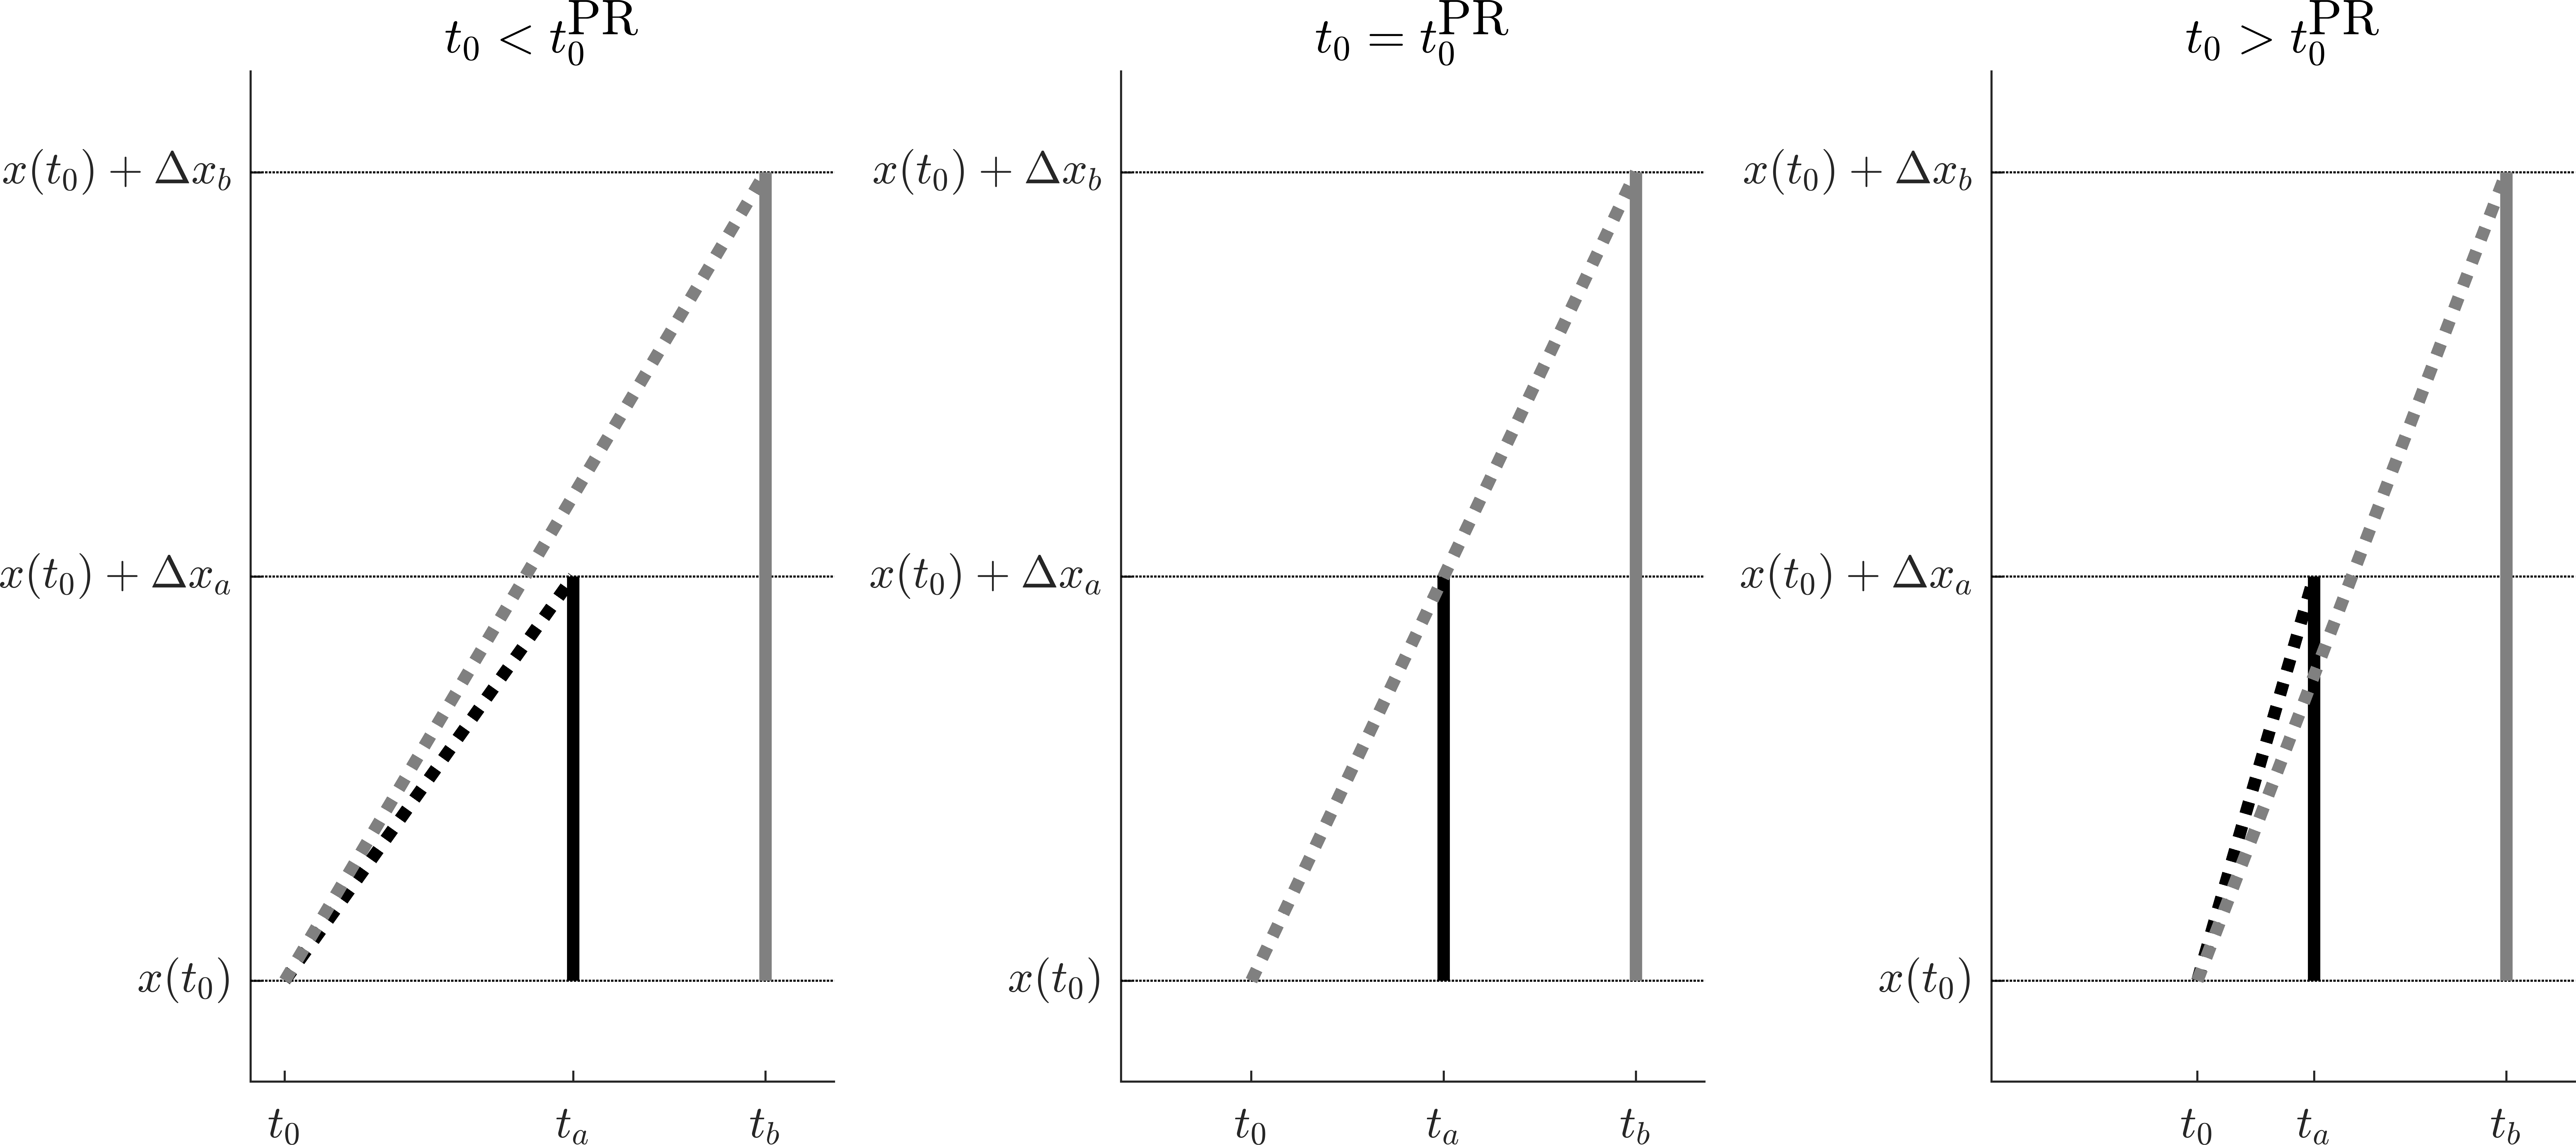
\includegraphics[width=1.0\textwidth]{./figures/caseC_reversal2.jpg}};
\draw [decorate,decoration={brace,amplitude=4pt,mirror},xshift=0pt,yshift=-5pt](-6.35,-3.15) -- (-4.7,-3.15) node [black,midway,yshift=-10pt]{\scriptsize $\hor$};
\draw [decorate,decoration={brace,amplitude=4pt,mirror},xshift=0pt,yshift=-5pt](-4.5,-3.15) -- (-3.45,-3.15) node [black,midway,yshift=-10pt]{\scriptsize $\del$};
\draw [decorate,decoration={brace,amplitude=4pt,mirror},xshift=0pt,yshift=-5pt](-0.15,-3.15) -- (0.9,-3.15) node [black,midway,yshift=-10pt]{\scriptsize $\hor$};
\draw [decorate,decoration={brace,amplitude=4pt,mirror},xshift=0pt,yshift=-5pt](1.08,-3.15) -- (2.13,-3.15) node [black,midway,yshift=-10pt]{\scriptsize $\del$};
\draw [decorate,decoration={brace,amplitude=4pt,mirror},xshift=0pt,yshift=-5pt](5.9,-3.15) -- (6.49,-3.15) node [black,midway,yshift=-10pt]{\scriptsize $\hor$};
\draw [decorate,decoration={brace,amplitude=4pt,mirror},xshift=0pt,yshift=-5pt](6.685,-3.15) -- (7.735,-3.15) node [black,midway,yshift=-10pt]{\scriptsize $\del$};
\end{tikzpicture}
\caption{Preference reversal in case C. From left to right panel, $t_0$ increases and $\hor$ decreases -- \ie both payments get closer -- while all other parameters are held constant. Initially, option $b$ is preferred, having the higher payment rate (slope of dashed line). At the critical time, $t_0=t_0^\text{PR}$, given by \eref{t0PR}, both options imply the same payment rate. At later times, option $a$ has the higher payment rate and is preferred.}
\flabel{caseC}
\end{figure}

Finally, we compute the discount function under this specification. When $g_a=g_b$, we have
%
\be
\delta\left(\del;\hor\right) = \frac{\Dx_a}{\Dx_b} = \frac{\hor}{\hor +\del} = \frac{1}{1+\del/\hor}\,.
\ee
%
Thus we recover the widely-used descriptive model of discounting in which the discount function, $\delta$, is a hyperbola of the delay, $\del$. We note that $\delta$ also depends on the horizon, $\hor$. Indeed, the degree of discounting parameter -- usually treated as a psychological parameter -- appears in our model as $1/\hor$, the reciprocal of the horizon \citep{MyersonGreen1995}. As the horizon gets shorter, $1/\hor$ becomes larger, $\delta$ gets smaller, and the later payment becomes less favorable. No knowledge of the decision maker's psychology is required in this setup, only the postulate that she prefers her wealth to grow faster rather than slower.

%\footnote{Indeed, the problem is fully specified by these two time periods and the two payment amounts. The actual times, $t_0$, $t_a$, $t_b$, are not needed to specify the problem because, when computing growth rates, only elapsed times matter. The time origin is arbitrary. Also, for this reason, $t_0^\text{PR}$, the preference reversal time in case C, can be negative if option $b$ is already preferred to option $a$ at the time of decision, $t_0$.}

Finally, we note that $k$, the underlying growth rate of the decision maker's wealth, does not appear in the decision criterion. This is because wealth growth is not affected by exogenous cash flows under additive dynamics: the gain $k\Dt$ over period $\Dt$ occurs regardless of other payments received. This contrasts with multiplicative dynamics, where early payments are subjected to the growth process through reinvestment.

\subsection{Case D -- Adaptive time frame with multiplicative dynamics}\label{sec:case_D}

Specification: the period for computing the growth rate is that between the decision and the chosen payment, either $t_a-t_0=\hor$ or $t_b-t_0=\hor+\del$; and wealth dynamics are multiplicative.

We follow the same steps as in the previous cases. Wealth evolves to:
%
\bea
x_a\left(t_a\right) &=& x\left(t_0\right) e^{r\left(t_a-t_0\right)} + \Dx_a\,;\\
x_b\left(t_b\right) &=& x\left(t_0\right) e^{r\left(t_b-t_0\right)} + \Dx_b\,.
\eea
%
The corresponding growth rates are:
%
\bea
g_a &=& \frac{\log x_a\left(t_a\right) - \log x\left(t_0\right)}{t_a-t_0} = \frac{1}{\hor}\log{\left(1 + \frac{\Dx_a}{x\left(t_0\right)e^{r\hor}}\right)} + r \elabel{ga_D}\,;\\
g_b &=&\frac{\log x_b\left(t_b\right) - \log x\left(t_0\right)}{t_b-t_0} = \frac{1}{\hor + \del}\log{\left(1 + \frac{\Dx_b}{x\left(t_0\right)e^{r\left(\hor + \del\right)}}\right)} + r\,.
\elabel{gb_D}
\eea
%

\subhead{Preference reversal}
When the later payment is sufficiently large, $\Dx_b > \Dx_a e^{r\del}$, preference reversal is predicted,\footnote{This can be shown by comparing the $\hor\to0$ and $\hor\to\infty$ limits of $g_a$ and $g_b$ in \eref{ga_D} and \eref{gb_D}.} and a threshold horizon, $\hor^\text{PR}$, exists. For shorter horizons than $\hor^\text{PR}$, the earlier payment is preferred ($g_a>g_b$) and \textit{vice versa}. The discount function and threshold horizon are not expressible in closed form for general parameter values. They become tractable in the limit of small payments, which we present below. If the later payment is too small, $\Dx_b < \Dx_a e^{r\del}$, the earlier payment is always preferred in this specification.

\subhead{Wealth effect}
Our model predicts another type of preference reversal here, elicited by varying the initial wealth, $x\left(t_0\right)$, rather than the horizon. As $x\left(t_0\right)\to0$, the earlier payment is preferred regardless of the size of the later payment. If the later payment is large enough, specifically if
%
\be
\Dx_b > \Dx_a e^{r\del}\left(\frac{\hor+\del}{\hor}\right)\,,
\ee
%
then it becomes preferable to the earlier payment as $x\left(t_0\right)\to\infty$. Thus, the decision maker switches from preferring earlier to later payments as her wealth increases. We label this the \textit{wealth effect}. It is illustrated pictorially in \fref{reversal_B}, which shows the variation of growth rates, $g_a$ and $g_b$, for each option as initial wealth, $x\left(t_0\right)$, increases from left to right. Other parameters are held constant.

\begin{figure}[!htb]
\centering
\begin{tikzpicture}
\node[inner sep=0pt] at (0,0)
{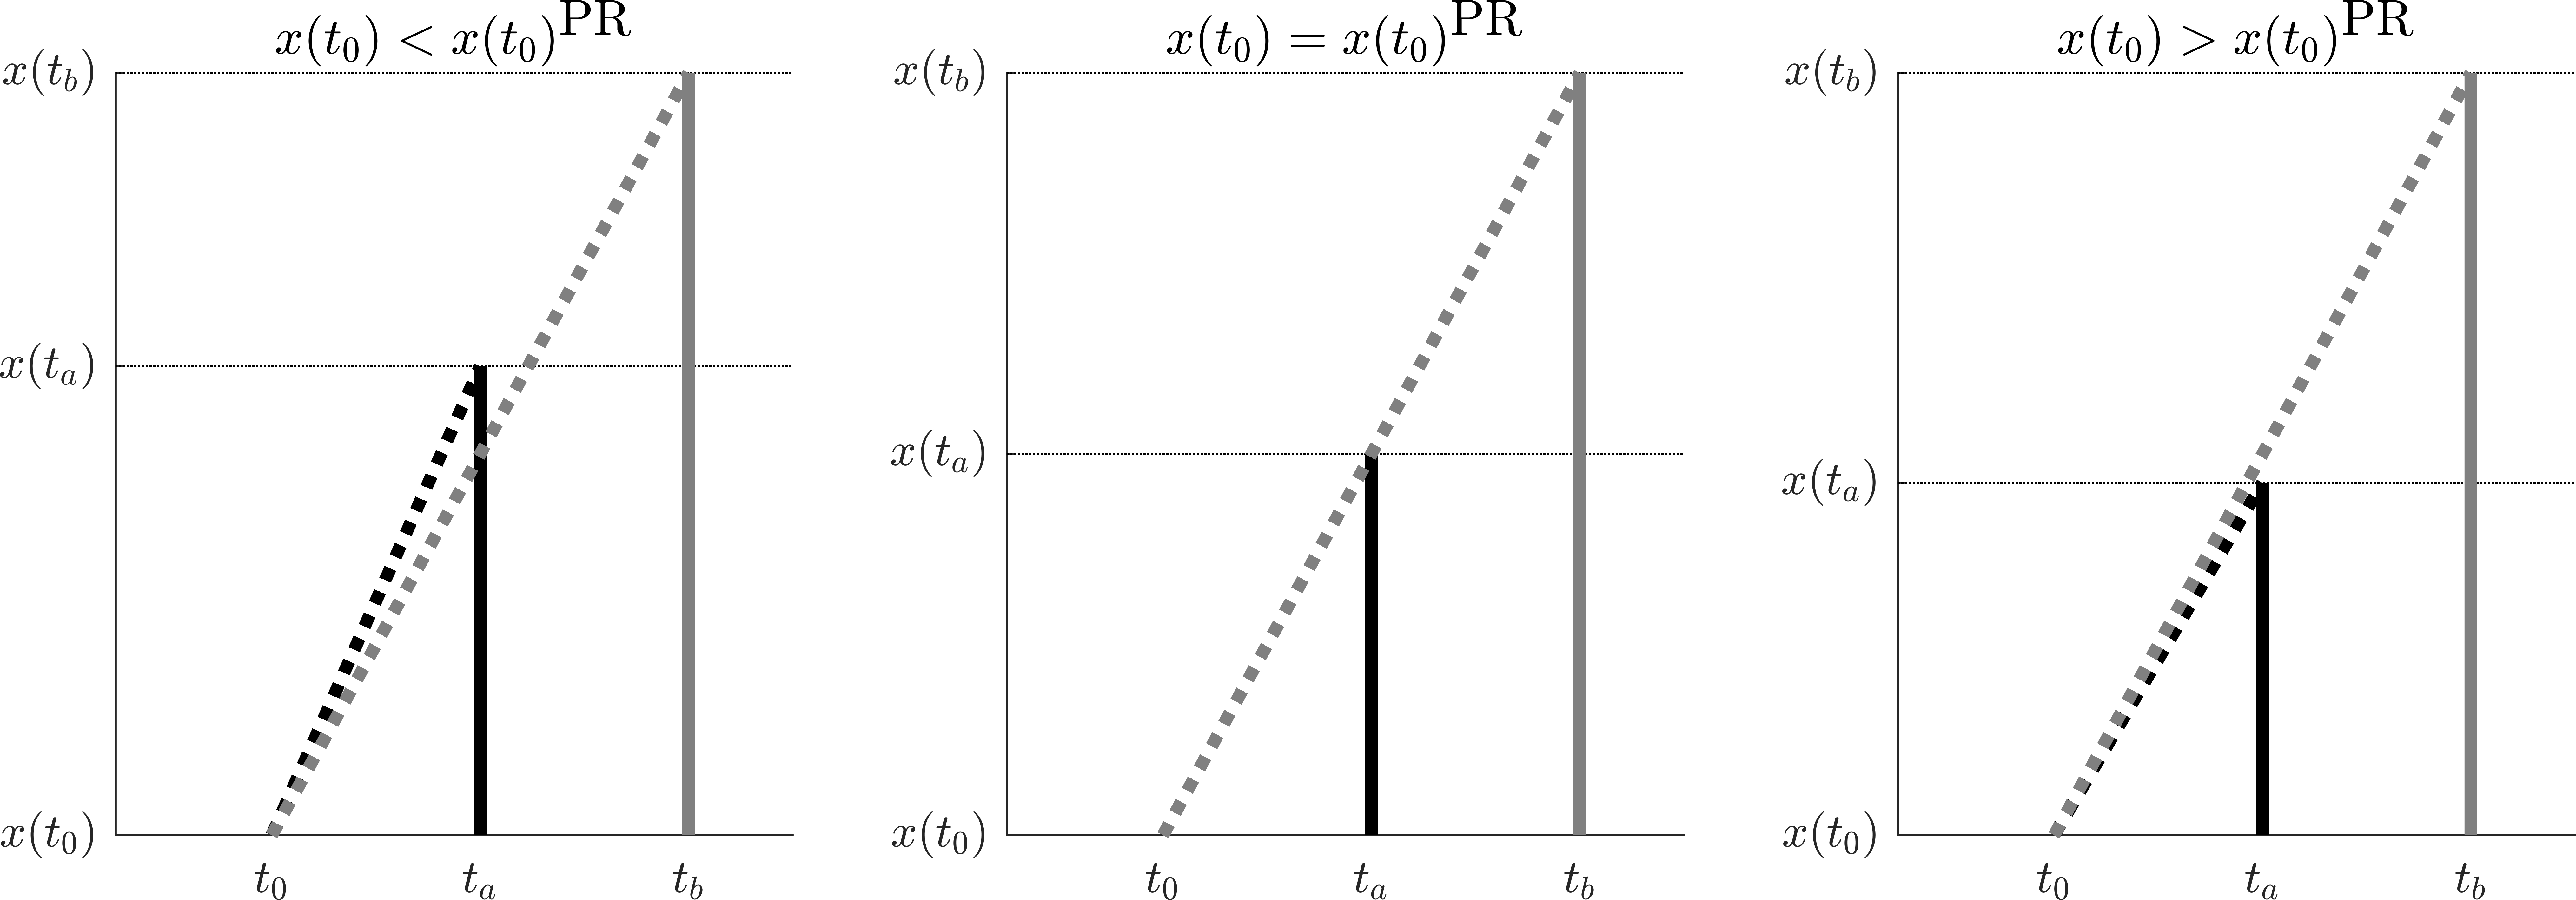
\includegraphics[width=1.0\textwidth]{./figures/caseD_reversal2.jpg}};
\draw [decorate,decoration={brace,amplitude=4pt,mirror},xshift=0pt,yshift=-5pt](-6.45,-2.38) -- (-5.32,-2.38) node [black,midway,yshift=-10pt]{\scriptsize $\hor$};
\draw [decorate,decoration={brace,amplitude=4pt,mirror},xshift=0pt,yshift=-5pt](-5.07,-2.38) -- (-3.94,-2.38) node [black,midway,yshift=-10pt]{\scriptsize $\del$};
\draw [decorate,decoration={brace,amplitude=4pt,mirror},xshift=0pt,yshift=-5pt](-0.72,-2.38) -- (0.41,-2.38) node [black,midway,yshift=-10pt]{\scriptsize $\hor$};
\draw [decorate,decoration={brace,amplitude=4pt,mirror},xshift=0pt,yshift=-5pt](0.66,-2.38) -- (1.79,-2.38) node [black,midway,yshift=-10pt]{\scriptsize $\del$};
\draw [decorate,decoration={brace,amplitude=4pt,mirror},xshift=0pt,yshift=-5pt](5.01,-2.38) -- (6.14,-2.38) node [black,midway,yshift=-10pt]{\scriptsize $\hor$};
\draw [decorate,decoration={brace,amplitude=4pt,mirror},xshift=0pt,yshift=-5pt](6.39,-2.38) -- (7.52,-2.38) node [black,midway,yshift=-10pt]{\scriptsize $\del$};
\end{tikzpicture}
\caption{Wealth effect in case D, with logarithmic vertical scales. Initial wealth $x\left(t_0\right)$ increases from left panel to right panel (\$500, \$2277, \$5500) with all other parameters held fixed ($t_0=$ today, $t_a=1$~year from today, $t_b=2$~years from today, $\Dx_a=\$1000$, $\Dx_b=\$2500$, $r=0.03$~per annum). At small wealth, option $a$ is preferred, having the higher growth rate according to \eref{ga_D} and \eref{gb_D}. At a larger wealth, $x\left(t_0\right)^{PR}\approx \$2277$, both options imply equal growth, with preference reversal occurring as wealth increases further. }
\flabel{reversal_B}
\end{figure}

\Fref{reversal_B2} shows the difference in growth rates, $g_a-g_b$, as a function of initial wealth, $x\left(t_0\right)$, for the same parameters as in \fref{reversal_B}. The earlier payment is preferred when this difference is positive, which happens for wealth below some threshold. For larger wealth, the growth rate difference is negative and the later payment is chosen.

\begin{figure}[!htb]
\centering
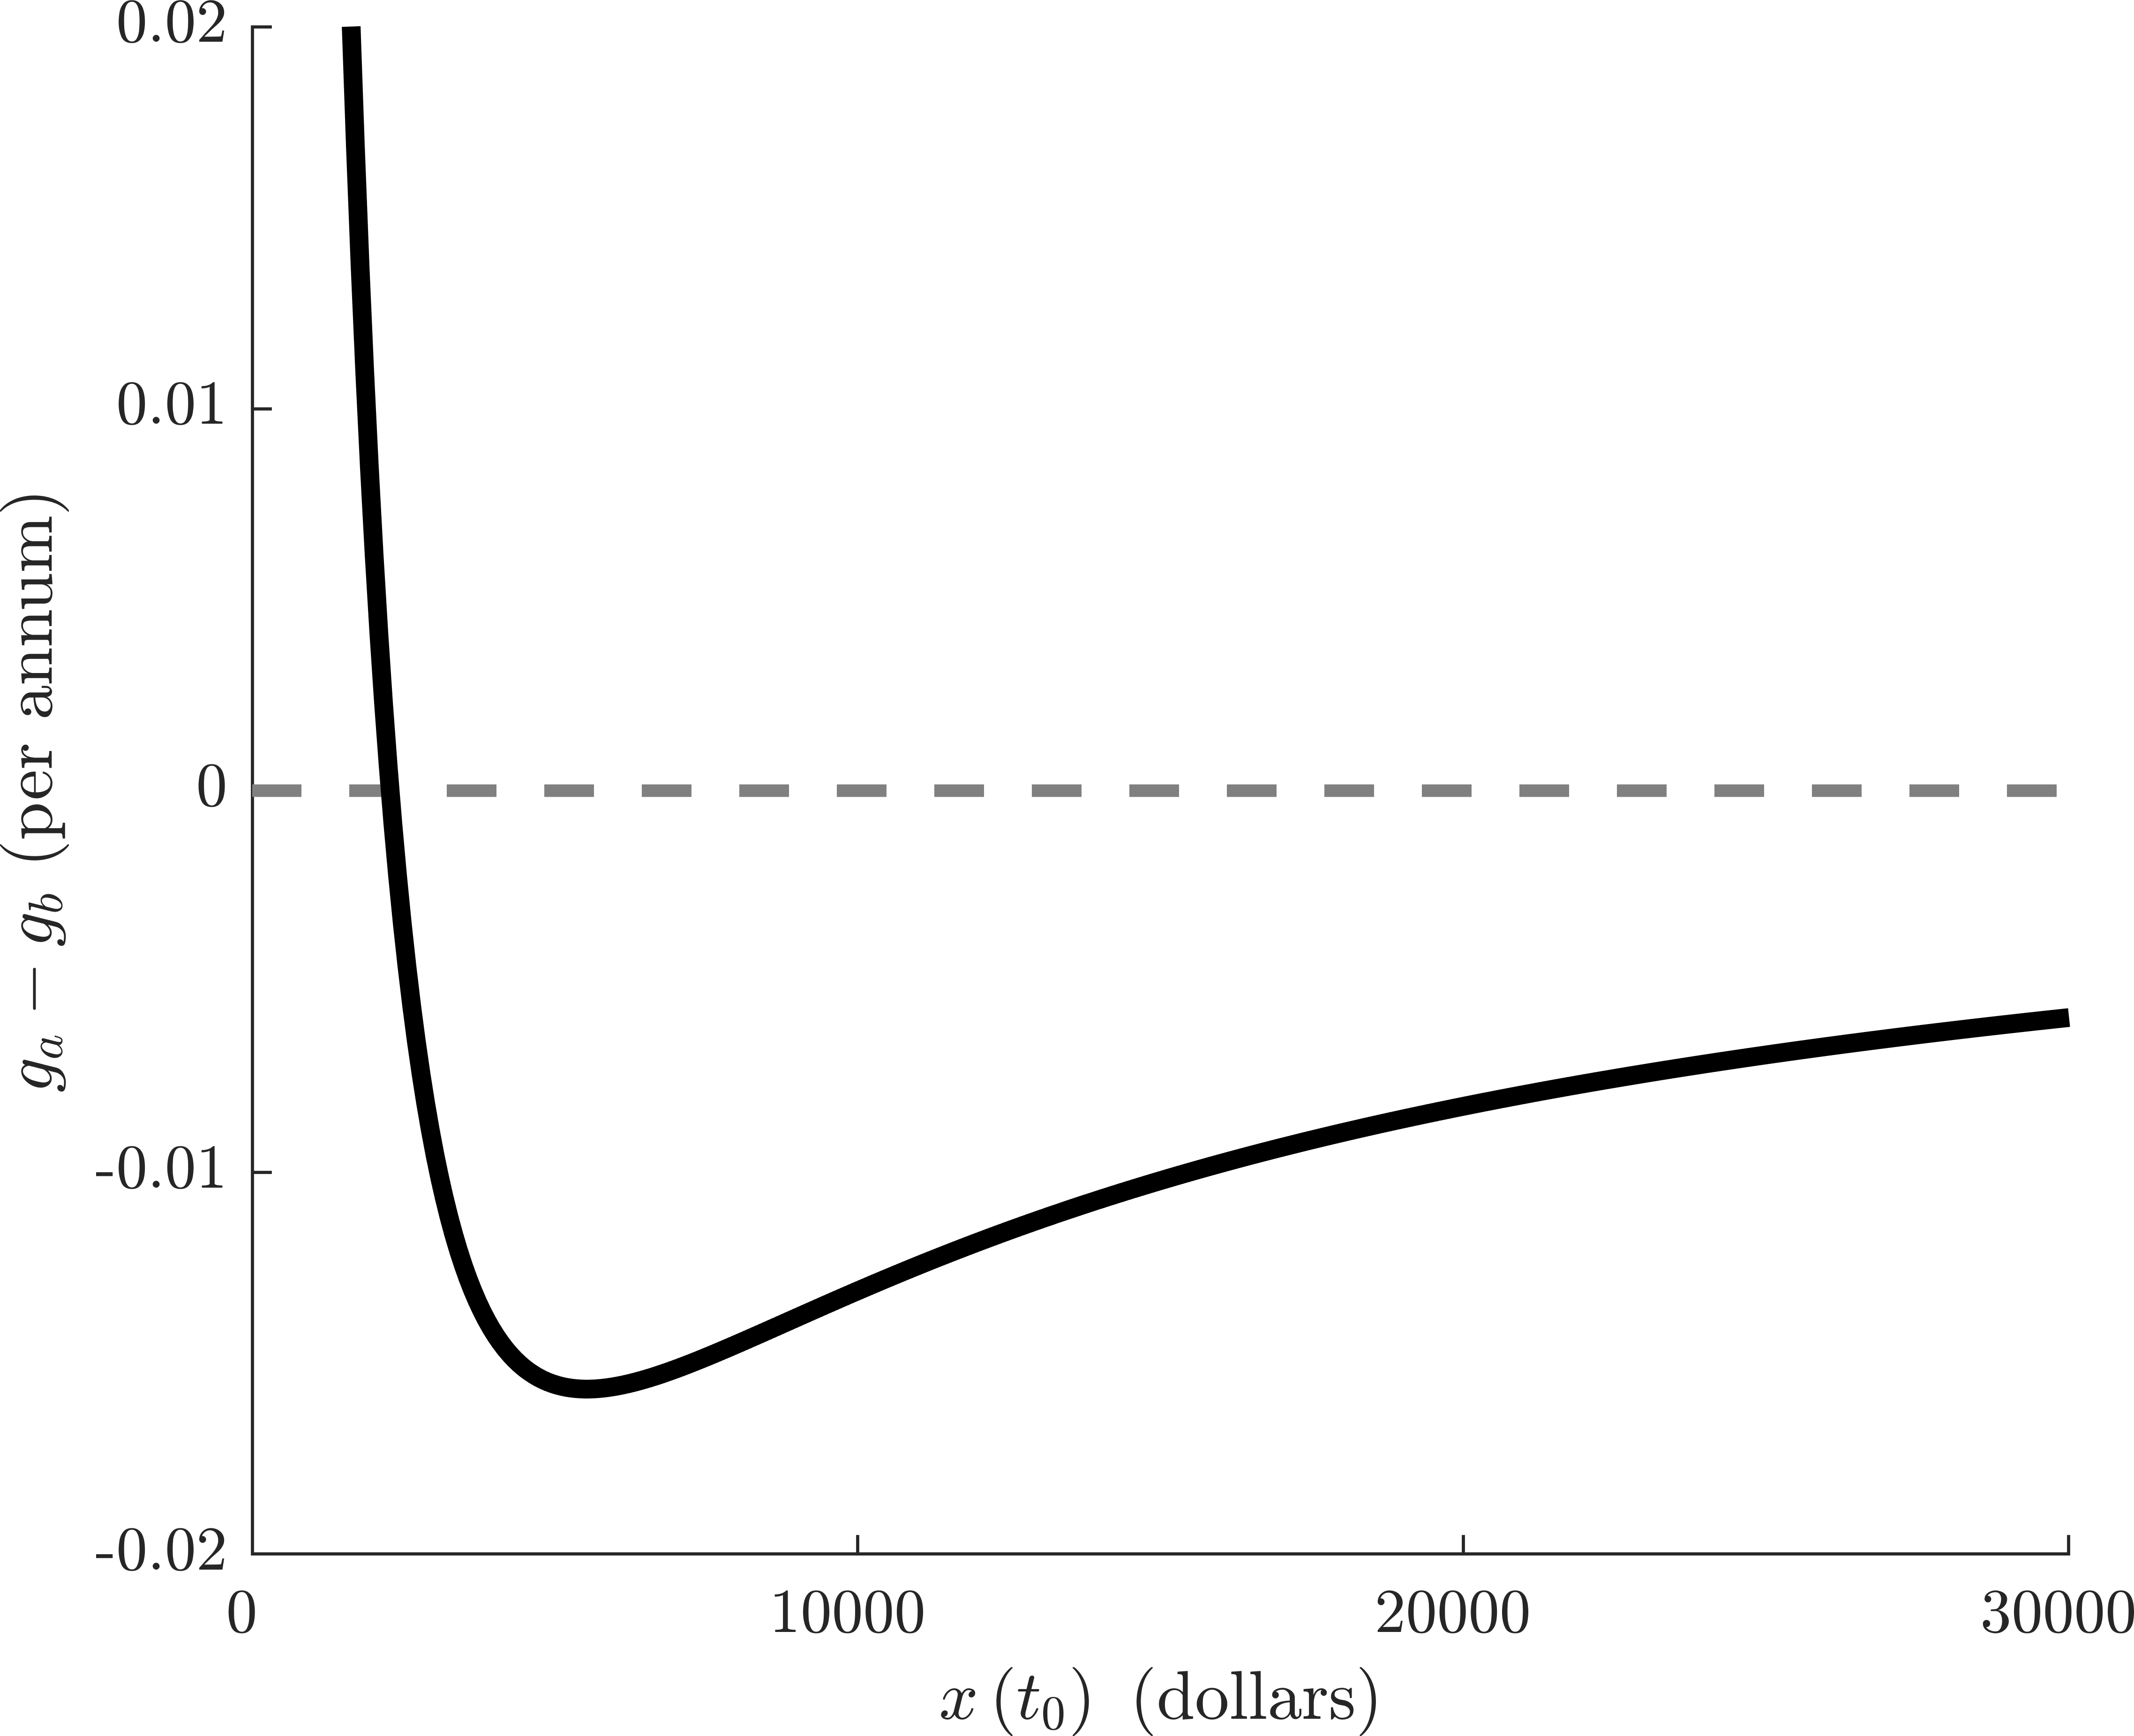
\includegraphics[width=0.7\textwidth]{./figures/caseD_ga_gb.jpg}
\caption{The difference in growth rates, $g_a-g_b$, as a function of initial wealth, $x\left(t_0\right)$, in case D. For small initial wealth the earlier, smaller payment is preferred, whereas for large initial wealth the later, larger payment is preferred. Parameters as used in \fref{reversal_B}.}
\flabel{reversal_B2}
\end{figure}

We interpret this as follows. Assuming multiplicative dynamics and an adaptive time frame, it is growth-optimal for people of lower wealth to choose an earlier, smaller payment; and growth-optimal for wealthier individuals to hold out for the later, larger payment. This is consistent with the findings of \citet{EpperETAL2018}, that ``individuals with relatively low time discounting are consistently positioned higher in the wealth distribution.'' It is likely consistent with \citep{GreenETAL1996}, in which people with higher incomes were observed to discount less steeply. 

We exemplify the wealth effect by presenting a calculation using the same parameters as in \fref{reversal_B}. Suppose a decision maker faces a choice between receiving $\$1000$ after one year (option $a$) or $\$2500$ after two years (option $b$), and that she has access to a risk-free interest rate of 0.03 per annum. If she has $\$500$ initially, she evaluates the growth rate corresponding to option $a$ as
%
\be
g_a = \frac{1}{1}\log{\left(1 + \frac{1000}{500e^{0.03\times 1}}\right)} + 0.03 \approx 1.1\text{~per annum}\,,
\ee
%
and to option $b$ as
%
\be
g_b = \frac{1}{2}\log{\left(1 + \frac{2500}{500e^{0.03\times 2}}\right)} + 0.03 \approx 0.9\text{~per annum}\,.
\ee
%
Thus, the decision maker would prefer the earlier, smaller payment, as $1.1 > 0.9$. If we assume that the decision maker had initially $\$5500$, \ie, 11 times more than in the previous setting, a similar calculation yields $g_a\approx0.19$ and $g_b\approx0.21$, so the later, larger payment is preferred.

\subhead{Discounting in the small payment limit}
In many applications of discounting, it is plausible to assume that the payments are small relative to wealth:
%
\bea
\Dx_a &\ll& x\left(t_0\right)e^{r\hor}\,;\\
\Dx_b &\ll& x\left(t_0\right)e^{r\left(\hor + \del\right)}\,.
\eea
%
We can express the threshold horizon and the discount function in closed form in this limit. Setting $g_a=g_b$ and using the first-order approximation $\log(1+\epsilon)\approx\epsilon$ for $\epsilon\ll1$, we get
%
\be
\hor^\text{PR} \equiv \frac{\del \Dx_a e^{r \del}}{\Dx_b - \Dx_a e^{r \del}}\,,
\elabel{HPRD}
\ee
%
and
%
\be
\delta\left(\del;\hor;r\right) = \left.\frac{\Dx_a}{\Dx_b}\right|_{g_a=g_b} \approx \frac{\hor e^{r\hor}}{\left(\hor + \del\right)e^{r\left(\hor + \del\right)}} = \frac{e^{-r\del}}{1+\del/\hor}\,,
\ee
%
which is a product of hyperbolic and exponential discount functions. This hybrid case has interesting behavior in the long- and short-delay limits. As shown in \fref{shortpaymentasymp}, discounting is close to hyperbolic for short delays and to exponential for long delays. Thus, for the same dynamic and the same time frame, and assuming small payments relative to initial wealth, our growth definition predicts both hyperbolic and exponential discounting, depending on the delay.

\begin{figure}[!htb]
\centering
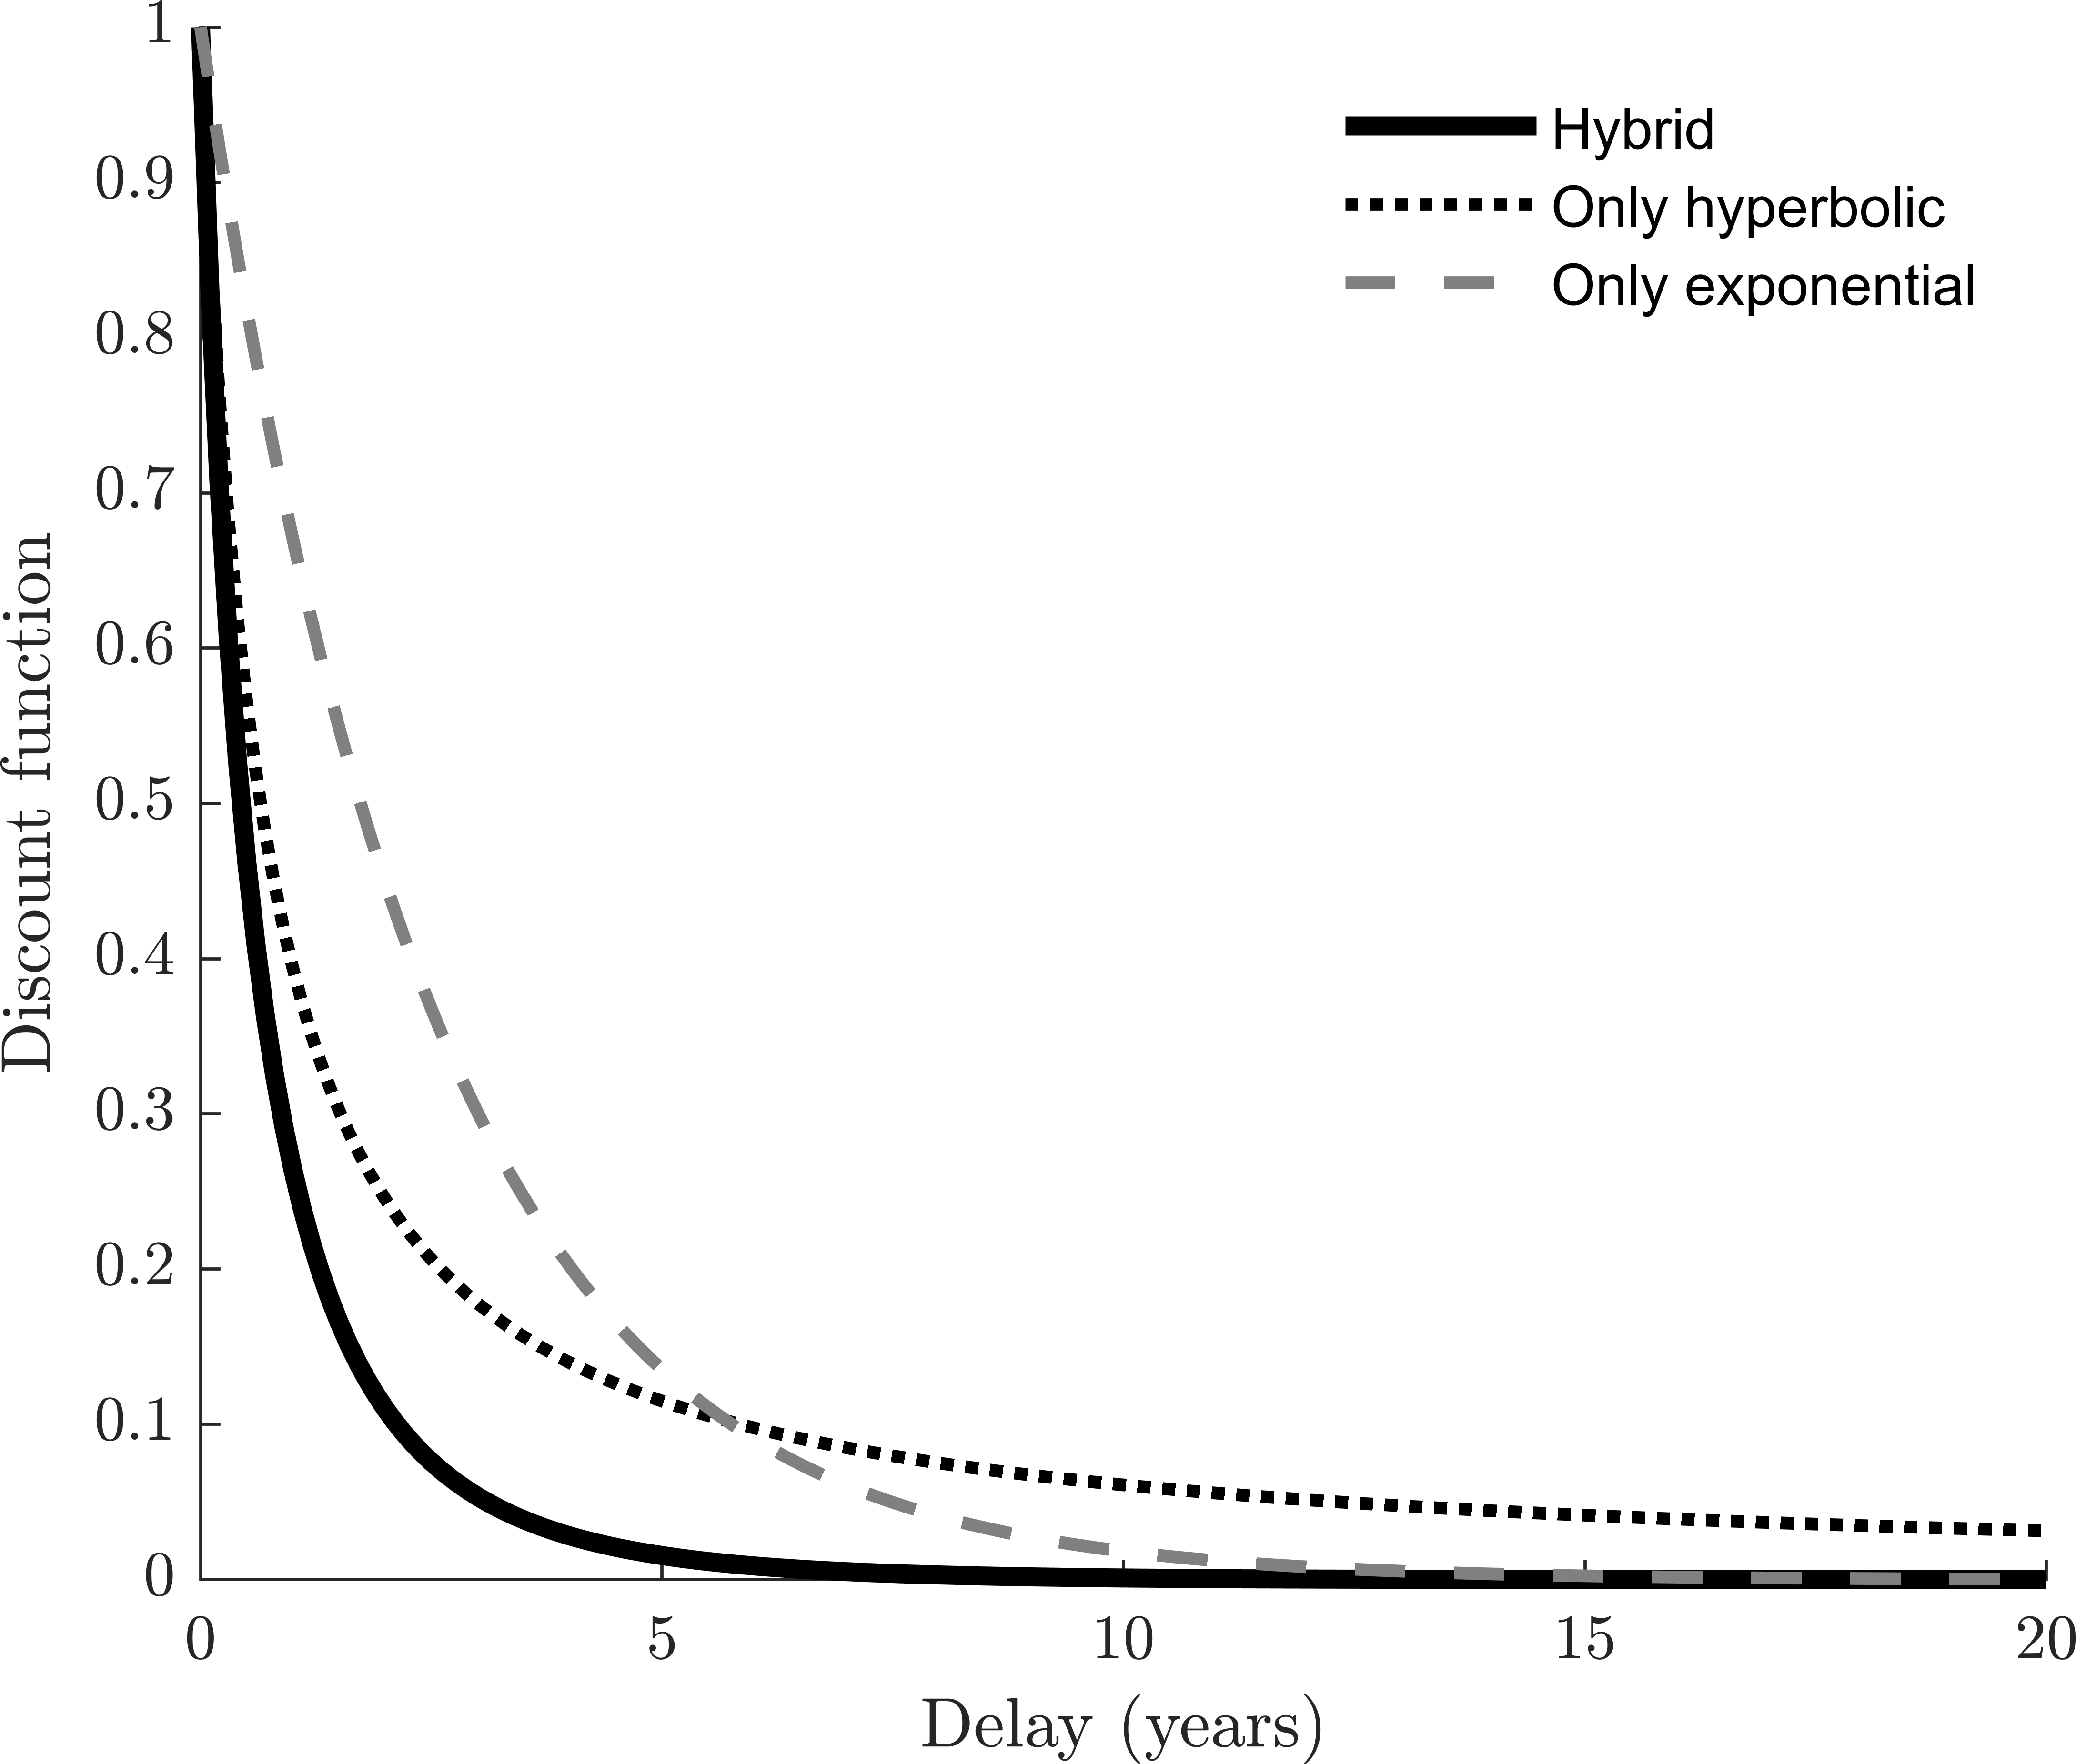
\includegraphics[width=0.7\textwidth]{./figures/caseD_delta_asymptotic2.jpg}
\caption{The discount function in the small payment limit in case D. The solid black curve is the hybrid $\delta = e^{-r\del}/(1+\del/\hor)$, for $r=0.4\text{ per annum}$ and $\hor=0.65\text{ years}$. This is close to the hyperbolic discount function $1/(1+\del/\hor)$ (black dotted) for short delays and to the exponential discount function $e^{-r\del}$ (grey dashed) for long delays.}
\flabel{shortpaymentasymp}
\end{figure}

%As before, only elapsed times, $\hor$ and $\del$, appear in the discount function. However, the background wealth growth rate, $r$, no longer cancels out when dynamics are multiplicative, as does $k$ when they are additive. This result gives a quantitative and falsifiable prediction of the circumstances under which one could expect to observe either hyperbolic or exponential discounting in the same setup.

\section{Discussion}\label{sec:discussion}

This paper explores temporal discounting under the postulate that decision makers maximize the growth rate of their wealth. We consider a basic temporal choice problem between two known, certain, and different payments at known, certain, and different future times. To compute growth rates, the problem must be further specified. We add information about wealth dynamics, treating additive and multiplicative cases, and the time frame of the decision, meaning the period over which growth is evaluated.

Preference reversal is an observed behavior in which decision makers switch from preferring later to earlier payments as time passes. It is incompatible with the classical normative model of exponential discounting. Our model generates four different forms of discounting, depending on the decision maker's circumstances -- no discounting, exponential, hyperbolic, and a hybrid of exponential and hyperbolic. The hyperbolic and hybrid forms predict preference reversal without, as is commonly needed, assumptions of behavioral bias or payment risk.

The hybrid case -- corresponding to multiplicative dynamics and an adaptive time frame -- suggests another type of preference reversal, called the wealth effect. Here a decision maker switches from an earlier to a later payment as her wealth increases. In other words, richer people discount less steeply than poorer people, in line with empirical findings \citep{GreenETAL1996,EpperETAL2018}.

Our main contribution is the prediction of non-exponential discounting and preference reversal in a model that does not violate standard axioms of choice \citep{vonNeumannMorgenstern1944}. Changes in the discount function arise only from changes in wealth dynamics and time frame. This marks a shift from psychological to circumstantial explanations of discounting. Our model assumes no dynamic inconsistency, in that the decision maker prefers at all times the option with the highest growth rate. If corroborated empirically, it would be both a normative and a descriptive model. Experimental tests are feasible because the model works directly with money payments rather than utility-of-consumption flows \citep{CohenETAL2019}.

The temporal choice problem we study is riskless. A planned extension of this work is to explore the consequences for our model of payment uncertainty. Uncertainty decreases the long-time growth rate associated with a payment \citep{PetersGell-Mann2016}. This would make a risky payment less desirable in our model, without reference to the risk preferences of the decision maker.

The dynamics discussed here do not cover the entire range of wealth dynamics. Although multiplicative and additive wealth dynamics are common and intuitive, other wealth dynamics are possible, which would lead to other forms of discounting in our model. Our decision criterion can be adapted to general dynamics using the growth rates described in \citep{PetersAdamou2018a}. 

%We also note that the fixed and adaptive time frames do not cover all possible time frames. In reality, time frames may overlap, \ie it is possible for a decision maker to decide on future payments before an anticipated payment has been paid already. For example, a manager makes a decision about a project, but before the chosen project is done and a payment received, a decision about other future projects is made. We leave the treatment of such cases for future work.

%We wish to emphasize that no knowledge of the decision maker's psychology is required in our setup -- only the postulate that she prefers her wealth to grow faster rather than slower. This postulate is enough for predicting a decision maker's discount functions used in standard discounted utility models. Yet, we also note that this paper discusses discounting from a theoretical perspective. An important complementary step of this research would be comparing the theoretical predictions of the results to empirical and experimental results. In particular, the predicted discount functions can be compared to results from controlled experiments. This is also planned for future work.

We end with a caveat. The temporal choice problem involves two {\it future} payments. In the small horizon limit, the growth rate corresponding to the earlier payment in the adaptive time frame diverges. This indicates a loss of model realism. We link this to the breakdown of an implicit assumption: that the growth rates we compute are sustained over sufficiently long periods to be meaningful to the decision maker. They are, in effect, the growth rates of wealth achieved under repetition of the choice. We share the view of \citet[p.~60]{Kacelnik1997} that ``the discounting process used for the one-off events seems to obey a law that evolved as an adaptation to cope with repetitive events.'' As the horizon shrinks, this imagined repetition occurs at a frequency so high that the choice problem no longer resembles a real situation.


\clearpage
\appendix

\section{The Transitivity of Growth Rate Maximization}\label{app:appA}

In this appendix we show that the maximization of growth, the growth definition in our model, satisfies transitivity for all four cases described in the paper. To prove transitivity we assume three vectors, $a\equiv\left(t_a,\Dx_a\right)$, $b\equiv\left(t_b,\Dx_b\right)$ and $c\equiv\left(t_c,\Dx_c\right)$, where $t_a < t_b < t_c$. We also assume a decision time $t_0 < t_a$ and an initial wealth $x\left(t_0\right)$. The vectors $\{t_a,\Dx_a \}$, $\{t_b,\Dx_b \}$ and $\{ t_c,\Dx_c \}$ are thus RIPPs.

In each of the four cases we will show that if $a \prec b$ under the RIPP and $b \prec c$, then $a \prec c$. We will also show that if $a \sim b$ and $b \sim c$, then $a \sim c$.

\subhead{Case A}
In case A (see \sref{case_A}), we show that growth rate maximization is achieved by choosing the larger payment. Therefore, $a \prec b$ iff $\Dx_a < \Dx_b$ and $b \prec c$ iff $\Dx_b < \Dx_c$. It follows that $a \prec c$ because $\Dx_a < \Dx_c$. If $a \sim b$ and $b \sim c$ then $\Dx_a = \Dx_b$ and $\Dx_b = \Dx_c$, so $\Dx_a = \Dx_c$ and $a \sim c$.

\subhead{Case B}
In case B (see \sref{case_B}), we show that growth rate maximization is achieved by comparing the earlier payment to the later payment discounted by an exponential function, so
%
\bea
a \prec b &\iff& \Dx_a < \Dx_b e^{-r\left(t_b - t_a\right)}\,;\\
b \prec c &\iff& \Dx_b < \Dx_c e^{-r\left(t_c - t_b\right)}\,.
\eea
%
It follows that $\Dx_b e^{-r\left(t_b - t_a\right)} < \Dx_c e^{-r\left(t_c - t_b\right)} e^{-r\left(t_b - t_a\right)} = \Dx_c e^{-r\left(t_c - t_a\right)}$, so
%
\be
\Dx_a < \Dx_c e^{-r\left(t_c - t_a\right)} \Longrightarrow a \prec c\,.
\ee
%
Similarly,
%
\bea
a \sim b &\iff& \Dx_a = \Dx_b e^{-r\left(t_b - t_a\right)}\,;\\
b \sim c &\iff& \Dx_b = \Dx_c e^{-r\left(t_c - t_b\right)}\,.
\eea
%
It follows that $\Dx_b e^{-r\left(t_b - t_a\right)} = \Dx_c e^{-r\left(t_c - t_a\right)}$, so
%
\be
\Dx_a = \Dx_c e^{-r\left(t_c - t_a\right)} \Longrightarrow a \sim c\,.
\ee

\subhead{Case C}
In case C (see \sref{case_C}) only the linear payment rate of each option matters to the decision maker, so
%
\bea
a \prec b &\iff& \frac{\Dx_a}{t_a - t_0} < \frac{\Dx_b}{t_b - t_0}\,;\\
b \prec c &\iff& \frac{\Dx_b}{t_b - t_0} < \frac{\Dx_c}{t_c - t_0}\,.
\eea
%
It follows that $\frac{\Dx_a}{t_a - t_0} < \frac{\Dx_c}{t_c - t_0}$, and $a \prec c$. Similarly,
%
\bea
a = b &\iff& \frac{\Dx_a}{t_a - t_0} = \frac{\Dx_b}{t_b - t_0}\,;\\
b = c &\iff& \frac{\Dx_b}{t_b - t_0} = \frac{\Dx_c}{t_c - t_0}\,,
\eea
%
so $\frac{\Dx_a}{t_a - t_0} = \frac{\Dx_c}{t_c - t_0}$, and $a \sim c$.

\subhead{Case D}
Like in case C, the time frame in case D (see \sref{case_D}) is adaptive. For this reason the growth rate associated with each payment depends only on the payment time and the decision time. In other words, under both comparisons between $a$ and $b$, and the comparison  between $a$ and $c$, the growth rate associated with payment $a$, $g_a$, is the same. Similarly, $g_b$ is the same in both the comparison between $a$ and $b$, and the comparison between $b$ and $c$. And $g_c$ is the same in both the comparison between $c$ $b$, and the comparison between $c$ and $a$.

It follows that
%
\bea
a \prec b &\iff& g_a < g_b\,;\\
b \prec c &\iff& g_b < g_c\,,
\eea
%
so $g_a < g_c$, and $a \prec c$. Similarly,
%
\bea
a \sim b &\iff& g_a = g_b\,;\\
b \sim c &\iff& g_b = g_c\,,
\eea
%
so $g_a = g_c$, and $a \sim c$.

\qed

\bibliography{../thesisbib/bibliography}



\end{document}
